\documentclass[12pt]{report}

\usepackage[margin=1.0in, left=1.5in]{geometry}

\usepackage{setspace}

\usepackage{graphicx}
\usepackage{subcaption}
\graphicspath{{./images/}}

\usepackage[
backend=biber,
style=numeric,
sorting=none
]{biblatex}
\usepackage{blindtext}
\usepackage{enumitem}
\usepackage{xcolor}
\addbibresource{references.bib}

\setlength{\parskip}{1em}
\setlength{\parindent}{0em}

% Title Page
\title{Robinson Observatory Telescope Refresh}
\author{Bradley Glaser, Derek McCrae, Bryan Ocbina, Justin Rudisal}

\begin{document}

\onehalfspacing

\maketitle

\begin{abstract}
The Robinson Observatory Telescope Refresh is an interdisciplinary project with Mechanical Engineers, Electrical Engineers, and Computer Scientists. The overall project will be focused on the creation of a sub-scale model. We will construct a working telescope model that will take in commands from an open-source telescope control program and position itself to those coordinates. As Computer Scientist, our first goal for this model will be connecting a control software to the model telescope. This software will send signals to an Arduino board that will interpret the signals and execute the slew commands properly with our specific motors and gears. The idea for this model is to show an implementation of a similar functioning telescope to that of the observatory proving the worth of an open-source telescope control program along with the understanding of the electrical complexity the observatory telescope houses.

The next goal of this project will be creating an application for the storing and viewing of photos taken by the observatory. Our database will organize the photos of the observatory based upon the metadata of each photo into a clean and easy to use UI. A stretch goal for this search functionality will be machine learning. Machine learning will allow the sorting of photos that do not include any metadata. The website will also include a community outreach program. The website

Finally, we will perform multiple activities on the enhancements of the observatory computer. First off, the computer needs to be updated to Windows 10. Its current version will soon be decomissioned by Microsoft. With this upgrade, we will need to ensure the computer retains its current functionality with all inputs and outputs of the computer. Next, we need to determine the functionality of their current server. We need to either find a new server solution for the observatory and their photos or regain the functionality their current server once had.

\end{abstract}

\section*{Executive Summary}

The Robinson Observatory Telescope Refresh is an interdisciplinary project between Mechanical Engineers, Electrical Engineers, and Computer Scientists. What once started as a project to repair the observatory telescope to its prior functioning state, has now shifted to the creation of a model. The complete project as a group is focused on the creation of sub-sub-scale model. The teams will construct a moving telescope model that will take in coordinates from a program and point to that location. The main goal of the model is to create a well documented project that works similarly to the observatory telescope to help in repair of the telescope. The telescope is very complex machine with the proper documentation to help in any repair. The model can provide test data for the observatory without the scale of the telescope or damaging the telescope any further. A second stretch goal is to create a telescope that others, willing to, can build. Our instructions in creating the telescope movement pieces and the software that accompanies would be available for anyone to view and use. As computer scientists, we are tasked with the telescope control software. Furthermore, our team will create a space photo web application based on the organizing of photos along with several observatory upgrades.

The telescope control program will be based on either an open-source program we find or one we create. The program will allow a user to select a point in the sky and then communicate with the Arduino board that will connect and control the telescope’s motors and gears. During communication between the two objects, the telescope will send its current location while receiving motor movement commands. The coordinates will need to be converted to motor instructions specific to the motors we use and gears we create to allow for proper function.

The next objective of this project will be creating an application for the storing and viewing of photos taken by the observatory. Our database will organize the photos of the observatory based upon the metadata of each photo into a clean and easy to use UI. A stretch goal for this search functionality will be machine learning. Machine learning will allow the sorting of photos that do not include any location metadata. The website will also include a community outreach program.

Finally, we will perform multiple activities on the enhancements of the observatory. First off, the control computer needs to be updated to Windows 10 as its current version will soon be phased out by Microsoft. Next, the observatory wants their server reconnected to the network. Their current server has not been used in years, which may cause the need to find a new server solution. Lastly, we will establish remote access of the control computer from the iMac downstairs. We will use the remote access ability provided in the Windows OS but will thus need to install Windows 10 onto the iMac.

\section*{Technical Content}

\subsection*{Project Narrative}

The Robinson Observatory is a facility at UCF that is used for both education and research on the topics of astronomy.  It is run by members of the Planetary Sciences Group and the Astronomy Society in the physics department.  The observatory provides high resolutions of astronomical objects and various events and programs involving the UCF and Central Florida to connect members of the community to astronomy .  The main telescope at the observatory is a 20-inch f/8.2 RCOS Ritchey-Chretien telescope and has recently had issues regarding its mobility.  The telescope is able to align itself to a starting reference point, but when given instructions to move to a certain coordinate, the telescope will unreliably move towards the coordinate without any relation to its physical capabilities or location.  This leads to a layer of issues.  The main issue involves being completely off-course of the desired coordinate.  The telescope software will either output warnings too early or too late and not prevent the telescope from colliding with its mount which causes damage to the entire system.  This is a hazard to the staff and the powerful and high cost telescope itself.

The origin of the problem is questioned whether it is a mechanical issue or a problem with the various software that are involved in operating the telescope.  Our computer science team alongside the electrical engineering and mechanical engineering teams will work together to determine the issues and provide solutions that will assist in leading bringing back the telescope to full functionality.  The main concern of the team at the observatory in regards to computer science is that the software of all of the components of the telescope are able to communicate properly on Windows 10.  The components are the telescope, TheSkyX Professional software, the focuser software, and the dome control software.  Meeting this specification will require research into each component of the system and also research into possible software/driver compatibility issues.  The knowledge to code drivers ourselves may be required.  Possible roadblocks may be that certain softwares are not updated or maintained to current standards which would require an overhaul of the system to have all components compatible.  Having the telescope and its surrounding system compatible will be the main objective of our project.

The second objective for our team will be to assist the research opportunities  and community outreach events available at the Robinson Observatory.  Our team will be designing a database capable of storing the images, and their metadata, taken directly by the telescope.  This database will function alongside a user-friendly website that can be used by the community for sharing images and also by the astronomer team to conduct research.  The images will be indexed with their relevant data and a search functionality will be available.  This will provide storage for the data collected at the observatory and assist in long-term research.  On the community side, the website will allow the observatory to easily share images with those interested.  A possible stretch goal is to use machine learning to search images for known objects based on a gathering of previous tagged images of the object.

The third objective will be to assist the electrical engineering team in modeling the black box which serves as the main component for issuing commands to the telescope.  The model will replicate the functionality of the telescope in turns of movement and sending and receiving data.  The current goal for the model is to be able to track the sun or moon within the accuracy of a degree.  This model will assist future teams as the complexity of the black box has been deemed to be too large in scope for a single year senior design team.  The reverse engineering of the black box will be useful for moving away from proprietary systems and give greater control to the team at the observatory in terms of what they would like out of the telescope, making it more programmable to their personal needs.

There are also a series of additional objectives pertaining to recording and storing astronomical data that will be obtained from the software when taking images.  They are outlined in the later sections of this document but serve to either allow for better research opportunities for the astronomer team or to simplify a process and improve the functionality of the facility through accessibility between systems at the observatory or allowing for online access to the faculty or community.

The refresh of the Robinson Observatory is a goal that is extremely important to each member of our team.  This project serves as an opportunity to give back to our university for all the experiences we have gained in our past few years here.  A reminder of all the knowledge we have accumulated into a single project demonstrating our technical skills and problem solving ability.  We hope to be able to remember our senior design project proudly as we bring an end to our time with education and proceed into the professional world of computer science.  Each of our members would also like to address their own personal interests and motivations in this project.

\subsection*{Personal Interest}

\subsubsection*{Justin Rudisal}

My personal interest in this project is twofold with the first part being due to the subject area being space, and the second due to the project area involving a level of mechanical integration. Within my own personal experience with Internships, I have worked heavily with website development and database management. However, I have absolutely no knowledge of mechanical systems and how a computer communicates with a physical, moving part. My dream goal is working in the creative entertainment programming field, such as Universal Creative or Disney Imagineering, and so I need this basic machine programming experience to be successful in my pursuit of a career in those areas.

I also have been in love with space and space exploration for as long as I can remember, and so much so that I originally was planning on doing a double major in both Computer Science and Astronomy until I sadly realized I could not afford to pursue both. So when I heard of the senior design project that would be combining both the area of knowledge that I wish to learn more in with an area of passion that I love, I knew I had to jump on it as quickly as I could.

Other major considerations of mine for this project include the fact that it is a completely open-source undertaking. The end goal of this is to be able to document and demonstrate everything we do so that other small observatories around the world can easily duplicate our results. Projects such as that are the ones that drive my passion in programming, as well as the engineering field in general, because I fully stand behind and support anything with altruistic goals that benefits other people for the common good. I personally believe intellectual progress is achieved from the sharing of knowledge freely, and not from the selling of it for a profit.

I also want to leave a legacy behind me within my university that I have called home for the past handful of years, and that has brought so many different opportunities into my life. I want to give back to the place that has given so much to me. Being able to refresh the telescope and have my name on such a substantial undertaking is one way that I can give back and leave that legacy. I can come back years later, point at the observatory, and say "I helped repair that and bring it into the modern era". Now that is both a great resume builder, and overall achievement to be proud to talk to others about.

I remember one of my most favorite experiences from my first years at college was actually going to the observatory for "Knights Under the Stars" throughout my first few semesters, and being able to watch the telescope work and see the screen show images of our galaxy. I thought that was one of the most fascinating things ever, and it sparked an even bigger passion in astronomy in my life. Lack of time, and it's breaking, caused me to stop going as I got into my higher level classes, but that initial impression left on me caused me to instantly want to help repair the observatory when it was announced as a senior design project.

\subsubsection*{Derek McCrae}

I want to embark on this project primarily for my interest in space. Growing up near the Kennedy Space Center, I was viewing the shuttle launches from a young age and dreamed upon what is out there. A sight I will always want to see firsthand has been strengthened by the pictures provided by telescopes. Telescopes provide a great photos of our universe that can't be currently reached by humans like the Hubble Telescope showcasing the Pillars of Creation or a simple home telescope to view Jupiter. This passion that has grown stronger with the advancements being made for commercial trips to space, especially the advancements by SpaceX. The technological advancements SpaceX has made with getting their boosters to land safely back at a landing pad simultaneously is one of the coolest things I have seen in the last decade. SpaceX along with Virgin Galactic have brought excitement back to space exploration. Some great memories I have include watch parties that had telescope viewings of either a launch, or eclipse, or viewing of another planet.

I had two events that greatly enhanced my passion for space. The first one happened when I was in 7th grade and our class trip was to the Kennedy Space Center. We were able to tour the facilities and sleep under one of the rockets that had on display. The trip helped gain new knowledge and greater appreciation of space. The second event happened freshman summer of high school on a trip to North Carolina. I was family on the side of a mountain in some cabins. One night the mountain staff held a viewing party. My family along with other guests were able to view the stars and use a telescope to see planets only viewable at that time of the year. The event showed me how the topic of space can bring people together.

These two events are a cornerstone to why I wanted to be apart of this project. I know firsthand how viewing parties can bring people together and the knowledge can be beneficial. Not many people own their own personal telescope so this observatory can give those interested a better way to view the sky. To know, I will have a helping hand in allowing activities to once again be performed at the observatory is exciting. The observatory can bring back “Knights Under the Stars” allowing many the current unavailable opportunity of getting to see the stars up close. The observatory could even provide new research study opportunities for those at UCF.

The next reason I chose this project was to build experiences on ideas I have yet to work with. My initial interpretation for this project was a new software needs to be created to help the telescope return to working order. I have learned how to code basic programs and taught programming stepping stones over the past few years without getting any real world experience. I have been eager to apply my knowledge to develop something that will be used past my educational career here at UCF. Furthermore, it will be applying this knowledge to help build something in an industry I am passionate about.

My final motivation for this project is the ability to leave behind a legacy. Of course, the legacy could become poor if this project isn’t completed properly but with proper completion, our solution will outlast my time here at UCF. This refresh could impact this university and space exploration for the next few years and that provides a strong legacy.

\subsubsection*{Bradley Glaser}

I have always had a deep love for everything space. Likewise, my science classes were always some of my favorite courses in school. From a very young age I was always asking questions and some of the biggest unanswered questions are extraterrestrial. The exploration and study of the cosmos must be one of humanity’s priorities if we are to advance as a civilization. I realize that my contributions to the Robinson Observatory are not quite earth shattering. However, I am happy to be able to say that I am a small part of that undertaking.

My father was always a very strong influencer in my life and he has always pushed me to pursue my goals. When I was in elementary, he got me my first childhood telescope. It was one of my most prized possessions. I kept it for many years and I have fond memories of stargazing with my friends and family. This project is an amazing opportunity to work on a full size telescope. One the day that we were assigned the projects, I called my father and told him about my selection. He was over the moon about it. I cannot wait to dig into this project and make it a reality.

My fiance and I have a special connection because of stargazing. When we lived in Utah, some of our earliest dates were spent on the top of a mountain looking at the stars and moon. We would hike up the mountain as the sun went down and then spend our time laying on the ground and watching for shooting stars. Our relationship was built on a shared love of science and space. Space has been a big influence on my life and I hope that my involvement in this project will help others to capture that same magic.

Intellectual property is a big concern of mine. I understand the value of having outside companies come to UCF and pitch projects. Students need real work experience and those businesses are able to provide it. However, the cynical side of me sees these businesses profiting off of the work senior design students are performing for them. Thus, I wanted to choose a project that would be internal to UCF. That way I can be sure that my time spent will not just be putting money into someone else’s coffers.

I wanted to work on a project that was tangible. Many of the projects presented for us to pick from were either esoteric or difficult to explain to non technical persons. Explaining that I will be on the team that fixes UCF’s observatory is immediately easy for anyone to understand. Likewise, I felt that potential employers would be more responsive to a project which was for the immediate betterment of others. It is hard for the average person to understand how “analyzing blockchain correctness” will affect them. However, I am able to point to the telescope and say “you couldn’t visit that before and now it works”. That direct impact is something that I wanted to have for a project.

Being able to contribute to UCF and help future students foster their love of astronomy is a dream come true. I hope that my contributions to this project will help others discover their passions. Similarly, the ability to leave a legacy behind at UCF is a big bonus. Many of the projects presented to us seemed fleeting or shallow in my opinion. They dealt with trivial things that, in the case of blockchain, might not even be relevant in the coming years. I hope that our contributions are more substantial and that they will stand the test of time.

\subsubsection*{Bryan Ocbina}

After hearing the pitch for this project, I realized being able to provide a meaningful impact on the UCF community was significant for myself.  I have grown up in Orlando all my life and have been ingrained to love all thing related to Florida from Disney and mickey mouse to the beaches and manatees to watching rocket and shuttle launches liftoff from Kennedy Space Center, with pure amazement every single time.  As I enter my final year as a Computer Science student, I would like to create a lifelong experience and memory here in my hometown before I finish my education, graduate, and begin to use my knowledge and technical skills in the professional world wherever my career may take me.  Aiding in the Robinson Observatory refresh is a project that aligns with my interests and goals and is my first choice amongst the about fifty projects presented to us.

One of my favorite memories is going on a camping trip a few summers ago and being to stargaze with close to zero light pollution.  The night sky at this time was and is still the most amazing and unforgettable sight I have ever seen.  I had a realization after seeing the sheer number of stars and the surprising amount of color of how much beauty we miss out on living in the city with lights everywhere.  Likewise, as another unforgettable experience was a viewing of a nighttime shuttle launch from my home in Orlando that lit up the sky as if the sun was rising.  Space and the stars above bring out childlike wonder in myself and brings excitement as our team begins to develop our design for the Robinson Observatory refresh.  To be able to once again share images from the telescope at the observatory and hopefully inspire some childlike wonder in someone else is an important part of this undertaking.

The UCF community and Central Florida as a whole is a wonderful center for growth and dreams.  Community outreach is a valuable aspect of this project.  Public events such as “Knights Under the Stars” held at the Robinson Observatory allow for people of all ages to explore the night sky and learn about our solar system and various nearby stars or other celestial phenomenon.  However with the main 20-inch telescope out of commission, the ability to view the night sky at these events is undoubtedly weakened.  We hope to not only restore this functionality but to also add on and allow for images from the 20-inch telescope to be shared more easily with the community.

As another part of community outreach, a decisive part of joining this project includes the open-source aspect of working with UCF.  This project serves to better the research opportunities available locally in Central Florida and our work done with the observatory will not be used to profit some business’s latest product.  The story of the project is much more involved and personal than the other projects pitched to our class.  We are able to not just present a fleshed out, functional telescope as a project we worked on but as an entire experience that could serve to inspire a future astronomer, aerospace engineer, or astronaut.

This project will be my number one priority for my remaining time as a student and I hope to gain as much as I can while working with everyone at the observatory and the other student teams as we share our experiences of our different fields and do our best to create an unforgettable experience.  Altogether, the Robinson Observatory refresh project serves as a platform to express my sincere appreciation for my hometown Orlando, Florida. I have many hopes for my senior design team that we will be able to accomplish some amazing features that will modernize the observatory and that will be used and remembered for many years after we have all graduated.  To be able to come back home, visit the observatory, and tell others that I worked on this feature or component at the Robinson Observatory would be a wondrous feeling.

\subsection*{Broader Impacts}

Laying the foundation down for getting the telescope and observatory working again will help with both the different organizations that contract out the observatory for their own scientific pursuits, as well as enhancing its ability to reach out to students and the surrounding community with an accessible means to the stars. Even those who are not local will be able to benefit from this project due to one of our goals being to create an online public viewing platform for what the observatory is currently observing and completing. This opens it up to anyone with access to an online device to actively engage with the observatory, as well as the scientific space community at large. Some goals is to create both an online portal for the observatories sponsors to access the information from the device, as well as crafting a learning environment for everyone.

This online outreach will also help spearhead engagement within space exploration and space overall within STEM groups both in the university as well as local elementary, middle, and high schools. Teachers will be able to pull up the current observatory pictures and developments, and will also be able to speak on weekly events that the observatory will be hosting. The overall goal is to both repair the observatory and bring it up to operating standards, as well as revamping its public outreach through new websites.

The organization that runs the observatory, Florida Space Institute, is a research group that is funded completely off of scientific grants and personal donations. By helping to repair this observatory for the Florida Space Institute we are helping an organization that may otherwise have a tough time affording the hiring of professionals to accomplish the intended goals. We are also helping to free up the time of those within the organization who may have had to spend their own time figuring out complicated temporary workarounds for the observatories problems instead of doing the scientific work that they want to accomplish.

Lastly the model telescope itself that we are creating will be entirely open-sourced. While the final release of the model telescope may not have the viewing capabilities of industry telescopes due to the nature of the project, we are designing our software in a way that it could work with telescopes with actual telescope-like viewing capabilities. A user will be able to tell our software what telescope they are using, so long as it matches the same type of motor movement as our model, and it will work for them like any other control software. The benefit is that our software will be free and open-sourced, and it will also be designed so that users can send the data from their telescope to any external location that they wish.

\subsection*{Requirements}

The CS team and engineering teams must coordinate together to solve many of the issues currently preventing the telescope from functioning properly. Thus, our project is unique in that some of our requirements might be solved by students from other teams working in parallel to us. Regardless of whichever team solves the problem, we will need to complete all of the requirements specified by FSI.
At the time of completing this document, FSI has not rendered up to date requirements for the scale model solution. Thus, these are the most current requirements. However, the CS team requirements are unlikely to be significantly altered.

\subsubsection*{CS Team Specific Requirements}

\subsubsection*{Essential Requirements}

The current control computer is running Windows 7. FSI would like the control computer to be upgraded to Windows 10. This presents several challenges. Firstly, we must ensure that “The SkyX Professional” control software is compatible with Windows 10. Likewise, there are several subsystems for controlling the mount, dome, focuser, and camera that must also be compatible with Windows 10. Similarly, the drivers required for the hardware components must be audited to determine compatibility and possibly replaced.

The telescope is currently controlled by a microcontroller “black box” attached to the mount. The CS team must ensure that any upgrades are able to communicate with said box. It is possible that the box might be replaced at some point in the future. Thus, it is important that the CS team understands and documents what signals are transmitted from the control computer to said box.

\subsubsection*{Secondary Requirements}

There is an iMac computer located on the lower level of the observatory. It would be nice if the observatory operators could control the telescope remotely from said computer. Investigating if a virtual machine or remote desktop software will be essential before we begin implementation. The sponsor seemed amenable to a remote desktop solution in order to reduce the number of computers directly controlling the telescope.

Setup a backup server at the observatory to store information gathered by the telescope. They currently have a server in the observatory but they do not know to what degree it is functional nor how the data is stored. We must investigate how it operates and possibly revamp their existing archive system.

Set up a online feed for sharing the most recent data capture by the telescope. As part of a community outreach effort, it would be nice if the public could easily view and interact with the photos generated by the telescope. We would have to convert the scientific specific files generated by the control computer into a publically digestible format.

Increase the accuracy of the control computer’s internal clock. At current, the observatory team is unable to perform certain time sensitive experiments due to the inaccuracy of the computer’s timekeeping. We must determine if the internal Windows method of synching the time can be overridden with a more accurate source.

\subsubsection*{Stretch Requirements}

The CS team would need to investigate the scripting capability of the existing control software. The observatory team had previously indicated that “The SkyX Professional” control software has the capacity to be extended/augmented via an existing scripting plugin. The CS team would need to investigate said system and determine the capabilities. The observatory team indicated that they may want basic functions automated if we have time.

\subsubsection*{General Requirements}

The dome subsystem needs to be controlled by the computer and integrate with the movement of the telescope. As the control software issues commands to the telescope controller, it must also issue corresponding commands to the dome subsystem. These components must both work in tandem or we will be capturing images of the inside of the dome instead of the stars.

The camera subsystem must be fully functional. Like the dome subsystem, it must communicate with the control software. The temperature, fan control, and camera calibration must be configurable and controllable. Finally, we must be able to accurately set the metainfo in the generated FITS file header generated by the control software.

The focuser subsystem will be a necessary part of capturing viable astronomical images which are fit for general consumption. It will need to be able to directly control the telescope’s focus from an integrated GUI. Likewise, the sponsor would like us to investigate the possibility of optimizing the autofocus routine. Finally, temperature fluctuations can impact the quality of images captured by the telescope. Temperature monitoring might be an option to automatically adjust the telescope focus to compensate for associated fluctuations.

The telescope subsystem controls the physical movements of the hardware. The control software must be able to execute the home and park capabilities of the telescope. Likewise, the control software must be able to send commands to the RA and Dec motors; the slew rates must be set in the control software. The telescope must be able to work in multiple modes. The first mode required is the sidereal tracking mode. Sidereal tracking mode fixes the signal going to the Dec motor, preventing it from moving, and only moves the RA motor tracks at sidereal rate. The second mode is the non-sidereal tracking mode. In the non-sidereal tracking mode both motors are moving at non-standard tracking rates. One area that the CS team needs to investigate is how the existing control software (The SkyX Professional) quantifies the non-sidereal rates. Likewise, we must investigate what units the software uses for said rates. Likewise, the telescope must be controllable manually by an operator directly. This performed via the use of an attached joystick and via the control software itself. At current, in the event of control failure, the telescope is in danger of damaging the both itself and the support infrastructure surrounding the telescope. This problem must be corrected with the use of pointing limits via the use of either physical limits or the control software. Finally, we must establish flip zone parameters near HA=0.

The filter subsystem controls the filters for the telescope. The filters are situated within the camera housing. The filter wheels get the power needed for operation from the camera subsystem. It is worth noting that the observatory has another filter wheel that is not currently connected to the telescope. We must be able to switch filters from within the control software. Research is required to determine if The SkyX Professional supports this operation natively or if we will need to plug into the control software’s scripting system to enable it manually.

\subsubsection*{Unofficial requirements}

We originally assumed that the telescope could be brought to a working state by the end of the semester. However, the electrical engineering team is unable to analyze and reproduce the necessary hardware in the span of a single senior design project. Thus our electrical engineering comrades will be replicating the motion of the telescope via a scale model. Their team (and possibly the mechanical engineering team) will develop a model which will be able to track celestial bodies in real time. Studying the movements of the model will help them better understand what an eventual solution to the telescope will entail. Thus, it will be one of the CS team’s responsibilities to create the software needed to track said celestial bodies as they pass across the sky. This tracking software will also need to be able to send instructions to the model so that it maintains a fix upon whatever celestial body is chosen. The CS team will be able to utilize the scale model to simulate inputs into any potential archiving software we will develop for the project.

\subsection*{Ideas}

Our first priority is coordinating with the interdisciplinary teams. Before any of the computer science team components can come to fruition, we must have a functional telescope to generate photos and associated data. Proper calibration and operation is the most immediate concern for our team. A study of “The SkyX Professional” software must be performed before we can assess what factors might be contributing to the current state of nonfunction. Likewise, it is possible that the issues currently plaguing the telescope might be a combination of many factors. Either way, the CS team must be prepared to coordinate and implement solutions in tandem with our engineering counterparts.

A community outreach website which would include both the existing data taken from the current Robinson Observatory website and a live/archived data component. The public data component would enable the public at large to have access to the data gathered by the observatory. Photos and positioning data would be presented to users when they access the website and it would be updated in near real time. As the telescope is operated, data gathered would be immediately available for public consumption. This functionality would have the ability to be enabled/disabled depending on the confidentiality requirements of the current research being done.

The current state of the telescope shows that it is able to calibrate to a reference point of Polaris, the North Star, but has no understanding of its position upon attempting to move to any other location.  A problem occurs when the telescope does not recognize it is reaching its mechanical movement limits to prevent damage to the telescope itself.  A possible solution consists of creating an emergency stop by coordinating with the other engineering teams and developing a functionality to have an emergency stop beyond currently pulling the plug to the motors.  There are some issues to consider when creating this as the telescope is very heavy and has many fragile components.  Moving the telescope requires a ramping up of speed and a deceleration time before coming to a complete stop.  This function would be useful for any hazardous conditions even when the telescope is properly functional.

Research is an important role at the Robinson Observatory.  The requirements for images and data to be accepted by the global astronomy community demand highly precise timings of exactly when the image is taken.  The telescope currently experiences issues with the timing requirement.  To solve this issue, we would like to be able to create some software that can accurately sync to an atomic clock and output the timing to the telescope image data.  This would provide the accurate timings required and allow for better research opportunities.  Another possibility would be to better the timing of the computer themselves to allow for the system to be more accurate.

Additionally there are servers at the Robinson Observatory that were previously used to store the data gathered from the telescope images. Their current state is not well maintained but we have been made aware that they do start up. Bringing back the servers to functionality would assist in research opportunities for the observatory while also creating a lasting system that could serve as storage for both long-term research and records. A fallback in case the servers are too damaged or unreliable would be to send the backup images to an offsite hosted server either as part of the UCF senior design hosting or to utilize a cloud storage solution. By collecting all of the photos in one place, we will be able to categorize them and make them more accessible to the researchers. Likewise, we might be able to generate new insights into their data via the use of machine learning. The ability to find patterns in existing data could open new avenues for future research to take place. In order to accomplish any meaningful machine learning, we must ascertain what types of research the existing staff does with their data, what their workflows are like, and how we can improve upon their methods with the application of computer science.

As the Robinson Observatory already has many chances for educational events, additional software or programs that would assist at these events would prove to be useful.  One idea is to provide quiz templates for information related to images capture by the telescope such as identifying astronomical objects ranging from planets, comets, stars, galaxies, etc.  There are many opportunities to provide additional activities at events such as Knights Under the Stars.

A possibility of being able to view images provided by the telescope in augmented reality at and around the observatory with simple description when interacting with the astronomical objects provides another technological experience for community members and to get more people interested in space and astronomy.  Interaction stations could be tied to GPS coordinates and provide short descriptions or quizzes at each station.  Some kind of reward for answering correctly and learning such as additional images from the telescope that players could keep.

Image analysis and machine learning for the observatory to be able to recognize various astronomical objects without having to specifically search and point at an object.  Space is full of objects and to be able to identify them quickly would be helpful for research and data collection overall.  This functionality would also serve to allow to automate processes for research by allowing long exposures of specific sections of the sky to be observed over a period of time for any anomalies or changes with known objects.

The addition of operating the observatory without someone at the facility could be useful to the observatory staff. To implement this feature, we have discussed using scripting and/or an application. Scripting was a feature the observatory once had so we could fix and build off that. Scripting would be the safest choice as no one could gain improper access to the telescope through an internet application. Scripting would allow someone to write a program that operates the observatory and t would be executed at a future set time. The other way for remote control would be through an internet application. The application would allow the user through proper verification to remotely control the observatory.

To tell the telescope where to point in the sky, some software needs to input commands to the telescope. Currently, the observatory uses SkyX Professional as it is the software provided with the Paramount telescope they purchased. It did work well for a while in the observatory but can only be used with the purchase of a black control box made by Bisque. In the hopes of ease and simplicity with the creation of our sub-scale model, we will use an open-source software to control the telescope. This will cut out the need for black box setup of the current observatory telescope that is creating control problems. There are multiple options for the telescope software that will be reviewed in the following paragraphs. The software will need to talk to an Arduino board.

The software for this sub-scale model, no matter which program chosen, will be pushing its outputs to an Arduino board. This board will essentially work like the black box in the observatory. It receives the information from the telescope software and translates that into operation code for the right ascension and declination motors. The Arduino board's software is written in C and has a plethora of libraries available online to use. We will need to equate the performance and counting of the motors to provide accurate instructions on what needs to move for how long or how much to achieve the proper positioning.

The software we end up choosing should not need modifications. The software just needs to be able to talk with our Arduino board in some way and present a clean, easy to use interface. Any modifications needed so the telescope moves on command from the software will be executed through the Arduino code.

\subsubsection*{Stellarium}

Stellarium is the first open source program we came across. Stellarium was a project started back in 2001 by Fabien Chéreau \cite{stell}. The software was first released in July of 2014 and had its most recent update in December of 2018. Each of its releases can be found on their github repository with a changelog. The software can run on Linux, Windows, or Mac so no compatibility issues will arise.

Stellarium at its core is used to show a 3D model of a realistic sky. You tell the software what you want to view and it creates a visual 3d output of the sky at that location. It is not a current view of that location. For tis project though, we need to push beyond this core use and use their telescope control feature that was implemented in version 0.10.5. The software allows you to control a GOTO telescope from the Stellarium UI. This feature sends movement commands to the telescope and receives the current position of the telescope. The feature is very simplistic but achieves the control we need for the project. Supervision will need to happen during telescope control though as movement will not stop even in the event of mount collisions or other safety events. It is also important tot note the telescope can end up being pointed at the Sun, which is dangerous to view at without the proper filters on a camera that is mounted on our model.

With Stellarium, the telescope control feature works in two ways: direct or indirect connection. Direct connection will send slew commands and positional coordinates of the model through LX200 protocol. This protocol sends two strings: one relates to right ascension and the other relates to declination. Depending on the type of mount used for the model, it may cause the need for conversions in coordinate systems. Stellarium only sends equatorial coordinates. These coordinates are a standard used by astronomers as it doesn't require constant recalculation. Since the sky is constantly moving, equatorial coordinates don't rely on the time aspect. The current observatory uses an equatorial mount so it works directly with equatorial coordinates. If the sub-scale model follows this mount, no conversions need to be made. However, if an altazimuth mount is used, conversions will need to be made in the Arduino software from equatorial to the altazimuth coordinate plane. Thus, it would be in the best interest of this computer science team to follow the current observatory mount into the sub-scale model.

\subsubsection*{Cartes du Ciel-SkyChart}

The next option available is Cartes du Ciel-SkyChart written by Patrick Chevalley \cite{skychart}. SkyChart's base use, like the name implies, is draw sky charts. A sky chart is similar to a map as it shows the location of stars in the current sky. This software is open-source and available on Windows, Mac, or Linux. Since this software is based in the drawing of SkyCharts, its open library has a plethora of information. People can upload their charts to the library for others to use. This mass database is useful for stargazing on specific stars and space areas, something our model will not need to feature. Our model will not have the camera range to prove if we are looking in the correct area for many of the charts available. This would be a great feature for the observatory though, as it has a camera strong enough for detailed viewings of space.

Through the use of these charts, the software allows you to control a telescope connected to the computer. To do so, the software can talk through the LX200 protocol like Stellarium. Furthermore, it supports INDI protocol for Mac and Linux while supporting ASCOM protocol for Windows. The ASCOM and INDI protocols are used to bridge the connection between control software and telescope. They are both open source frameworks designed specifically for the astronomy field.

SkyChart adds more options for how to send data between the software and our telescope. These protocol options would be more helpful though with the observatory telescope. The sub-scale model will be very simplistic in features. We do not need to worry about camera focus or dome control like the observatory does. These features would find use with the INDI and ASCOM protocols as you can send more information between telescope and software. As we only need slew commands and position strings, the LX200 protocol is still most useful for the model.

\newpage %Page break


\section*{Block Diagrams}

Our design has three distinct parts that make up the entirety of our project. The main goal of our project is to create functioning model telescope that can mimic the movement of the Robinson Observatory telescope so that it can be used as a reference to repair the observatory itself that is unable to move properly in it’s current state. The term “telescope” will be used throughout this paper, but keep in mind that the idea behind this model is to use it to backwards engineer the movement of the observatory’s telescope and not it’s viewing capabilities. Therefore, while we have a stretch goal of implementing a way to view images on our model telescope through the means of some sort of camera device, we are focused primarily on the telescope’s movement.

With that being understood, our three main parts of the project is creating the control software for the model telescope, creating a frontend website that can take the observatories data (i.e. image files, space observation information, etc) and present it in an easily accessible and searchable manner, and a backend system and server to keep track of all of that data and communicate with the frontend. A main stretch goal that we have is to integrate the website with the model telescope control software in a way that if the model telescope has imaging capabilities, we would want it to be able to directly store that in a way that the website can directly pull from it so that all three pieces can communicate with one another.

We are developing the control software to have the capability to point it’s output data to any server that the user specifies, and so we are using this design to aim for the target of reaching our stretch goals of implementing some sort of camera system into the telescope itself. The following diagram demonstrates our overall project flow and how each part works with one another.

\newpage


\begin{figure}[h]
	\centering
	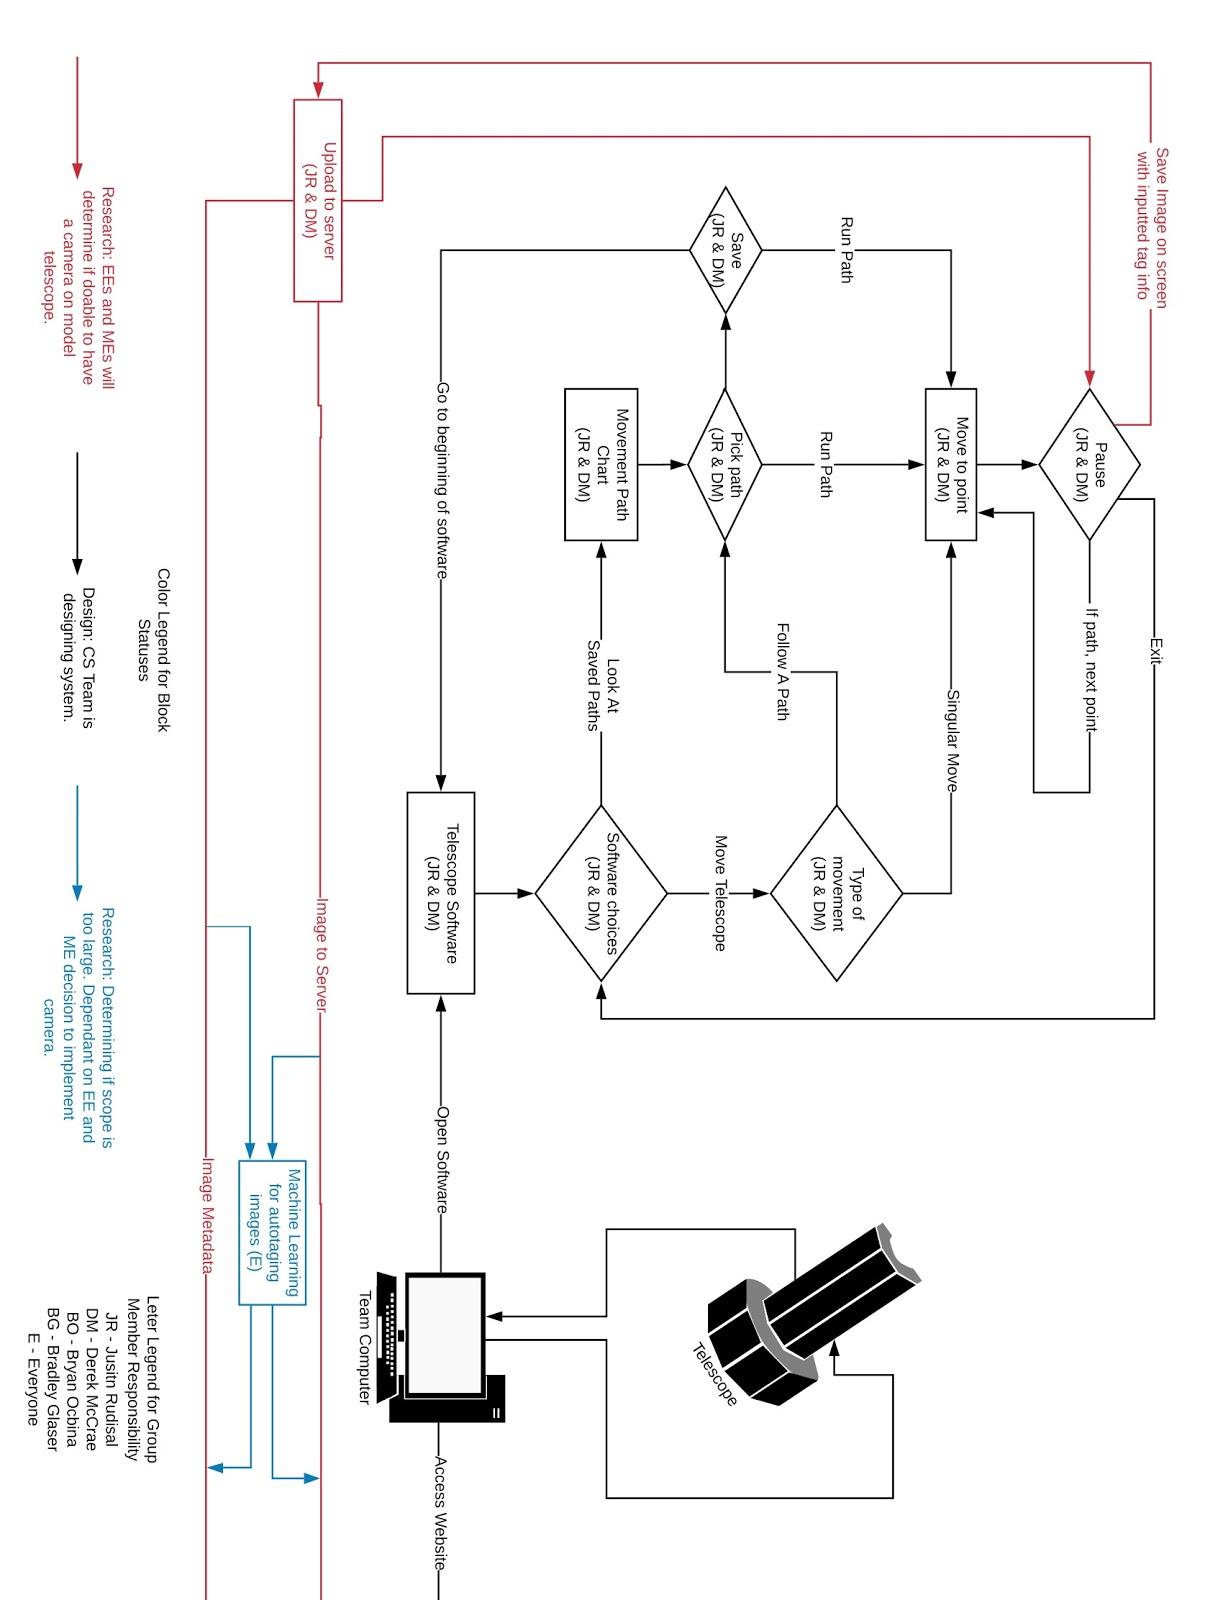
\includegraphics[width=1.00\linewidth, height=17.0cm]{blockpt2}
\end{figure}

\newpage

\begin{figure}[h]
	\centering
	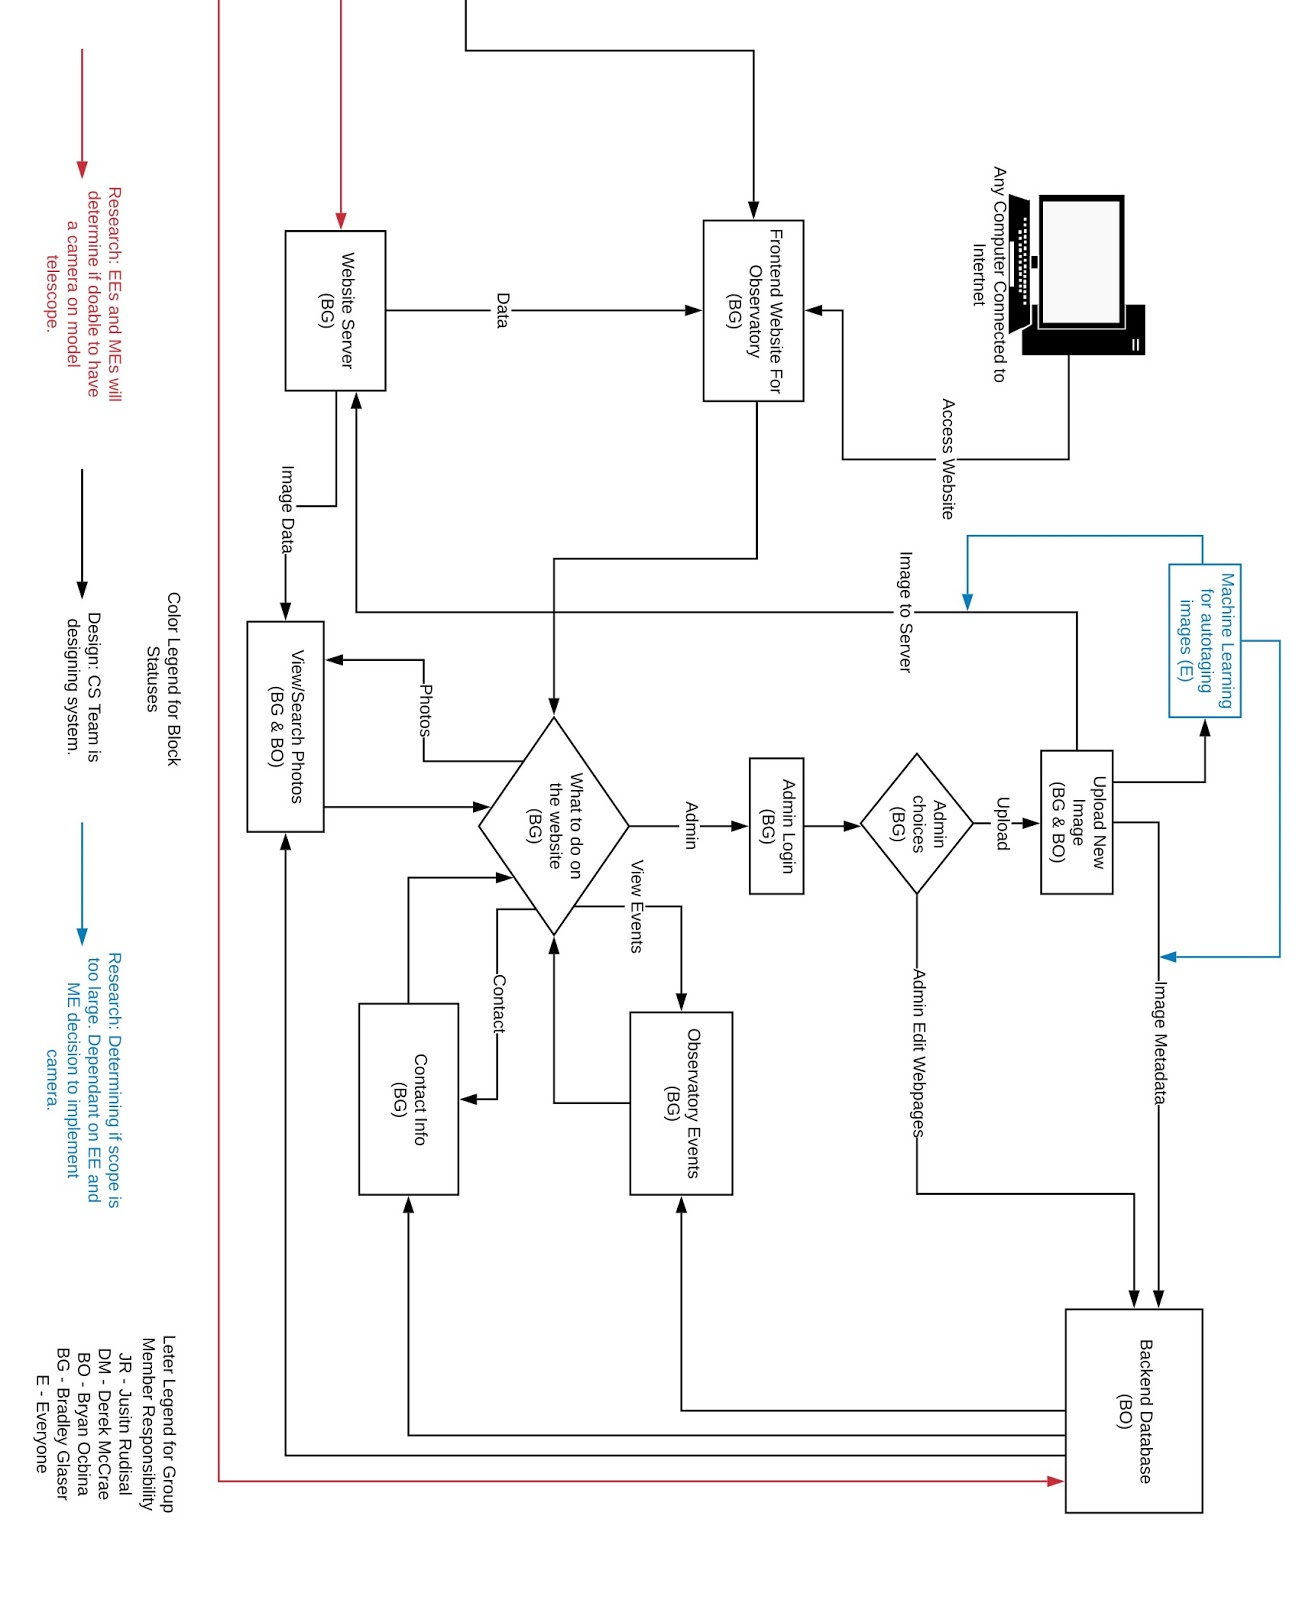
\includegraphics[width=1.00\linewidth, height=17.0cm]{blockpt1}
\end{figure}

\newpage

\subsubsection*{Challenges}

The first challenge, and in my opinion biggest, will be relating software commands to telescope movements. As a computer scientist, we mostly live our lives in a virtual realm. However, this project is breaking that barrier. Our software development will have a direct impact on the movement of the model telescope. We need to find a turn the strings of code into proper movements based on our specific functionality of the telescope. With our telescope being designed from the ground up, the gear ratios and motor torque will be unique. So, the Arduino board will not be able to directly execute the strings given by the software we choose. We will need calculations for moment of inertia, friction, and the impact of gravity on our model. Luckily, I have taken some mechanical engineering courses that dealt with these topics allowing me to have confidence tackling these issues.


\section*{Model Telescope Control}

\subsection*{Model Telescope vs Observatory Control}

The underlying premise that drives the need for our model telescope is to replicate the control structure that the Robinson Observatory currently has in a scaled-down and testable environment. The observatory is currently controlled by a software and hardware system known as SkyX Professional, which is a commonly used product for small observatories around the globe that helps individuals get their observatory telescopes operating to their fullest extent. However, while this software is extremely useful for the observatories purposes, it is actually a hindrance for our scale model. SkyX Professional does not translate well when being adapted to small-scale custom designed telescopes. By our understanding based on documentation, as well as the physical systems currently in the Robinson observatory itself, the software has a required hardware integration to use the SkyX software for the purposes of controlling the observatory. Without this hardware, the program is nothing more than a glorified virtual observatory software for a computer with no physical controls.

To further explain, this hardware integration is not designed to be used with telescopes that have been fully planned and created from scratch. The main issue lies in that a custom telescope would have its own custom inputs and outputs based on the needs of the creator, while SkyX and its hardware is designed to integrate with well-established brands and models. The actual SkyX software and what it’s sending out and receiving form the observatory telescope is hidden behind a layer of proprietary silence, and so therein lies the need for a custom model telescope control system. We cannot use SkyX as the observatory currently uses it because we are unable to tell what the software and hardware are communicating to each other beyond our reasoning of what we think it might be sending. Assumptions can be the downfall of projects, and so we decided as an interdisciplinary team to completely circumvent SkyX and create our own software.

\subsection*{Designing the Model Telescope Control Environment}

With the realization that we could not go the SkyX Professional route for our model telescope also came the realization that we would have to create our own custom telescope control software from scratch. Before doing any further research into what our software will do and how it will function, we first established as a team that this custom software will be open-source and easily transferable from our scale-model telescope to any real telescope. The idea behind this is that we want to be able to take our software and have senior design teams after us be able to use it as a well-defined base for repairing the Robinson Observatory. The entire thought-process behind the scale model to begin with is due to that fact that there is no currently established base, and so our team has no reference from which to repair the observatory ourselves as it stands. The hope is that with this software and model in place, future teams will have a working base form which to build off of.

After some brainstorming and hashing around ideas, our team established that there would be little difference between our model telescope and a robot. In fact, our telescope would essentially be a controllable robot. With this in mind, we realized that we needed to establish a base software from which to do this controlling from. Taking the stance of this being a robot, we are now also free to test our designs entirely within a simulator environment to ensure our software will actually work with the physical custom model telescope.

The following sections will discuss our plans on creating our software to control our robotic telescope. Further sections will then discuss how we plan on testing our software using a simulator environment.

\subsection*{Creating our Telescope Control Interface}

\subsubsection*{High-level Overview}

Our software will be a C++ open-sourced console application, which we will be developing in Visual Studio. We envision the application to have four base functions which are coordinate inputs to make the telescope go to a singular point in the sky, object tracking to follow an object once given it's initial position, customizable settings, and saving and loading of previously tracked objects. There is also the element of having a camera, such as a GoPro, attached to the telescope to demonstrate a visual aspect. However, this is largely dependent on the other interdisciplinary teams integrating it into the telescope and is seen as a fun stretch goal. We will design our software to include the ability to use a camera, but our project's custom telescope may not actually have one. Again, the emphasis is on the movement of the telescope and not the actual ability to view the sky. The following three sections will go into details on what each base function will entail, including mock-ups that we have created of what we envision each part will look like. Following these sections will be a further explanation of exactly how we will create this application.

\subsubsection*{Singular Point Movement vs Tracking Movement}

The main use for our model telescope will be to demonstrate the movement functionality of both our interdisciplinary teams hardware and our computer science team's software. With that being understood, the most important feature of our software is moving the telescope to focus on a single point in the sky in order to demonstrate proper movement. It will very much resemble a 'point, click, and go' method of movement. This will be accomplished by first using the aforementioned open-sourced software Stellarium to pick a point in the sky in order to pull the equatorial coordinates of that location. Once our software has those coordinates, the user will be able to decide if they want to move the telescope to this position without tracking, or move to this position and follow that point in the sky as the Earth rotates by choosing the tracking option.

The user interface for this functionality will be very simple and to the point (Figure 1). Stellarium gives a beautiful virtual planetarium of the sky from wherever you are by taking your device's current location, or a location that the user specifies. Our software will plug into Stellarium via a toggle on the bottom taskbar of the program. When toggled on, a console application will appear showing the main screen of our software. As shown below, this will give the current equatorial coordinates of what the user has picked on the virtual planetarium. It will show empty coordinates if the user has yet to pick anything. The chosen point in the sky is denoted by a bullseye icon on the planetarium.

\begin{figure}[h]
	\centering
	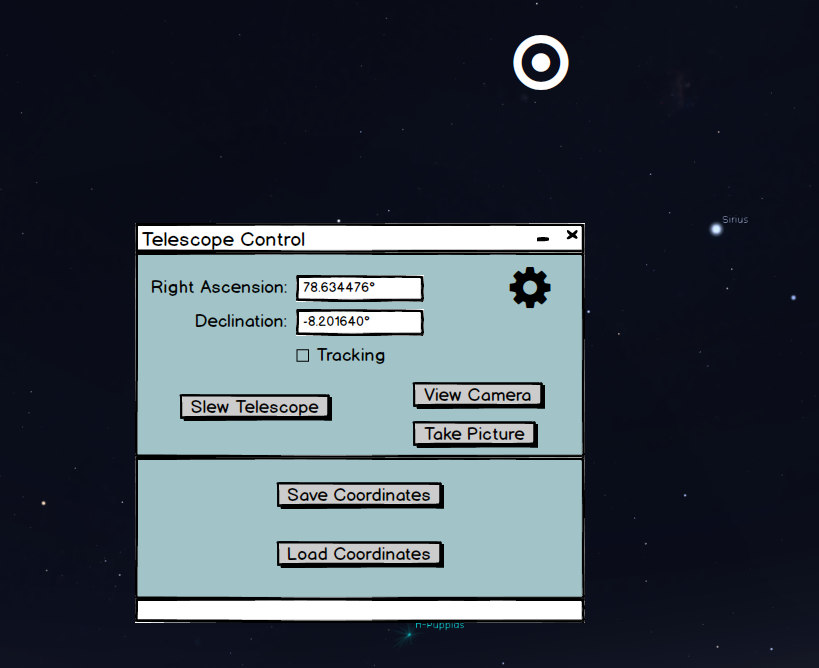
\includegraphics[width=0.85\linewidth]{MainScreen}
	\caption{Main screen of telescope control}
\end{figure}

The user will be able to move the telescope by clicking the 'Slew telescope' button when there are coordinates in the coordinate textboxes. If there is a camera currently attached, they will also be able to view whatever their current camera is visually seeing (Figure 2) as well as take a picture of the camera's view of that exact moment in time. These can be stored both externally as well as locally, and this will be explained later.

\newpage

\begin{figure}[h]
	\centering
	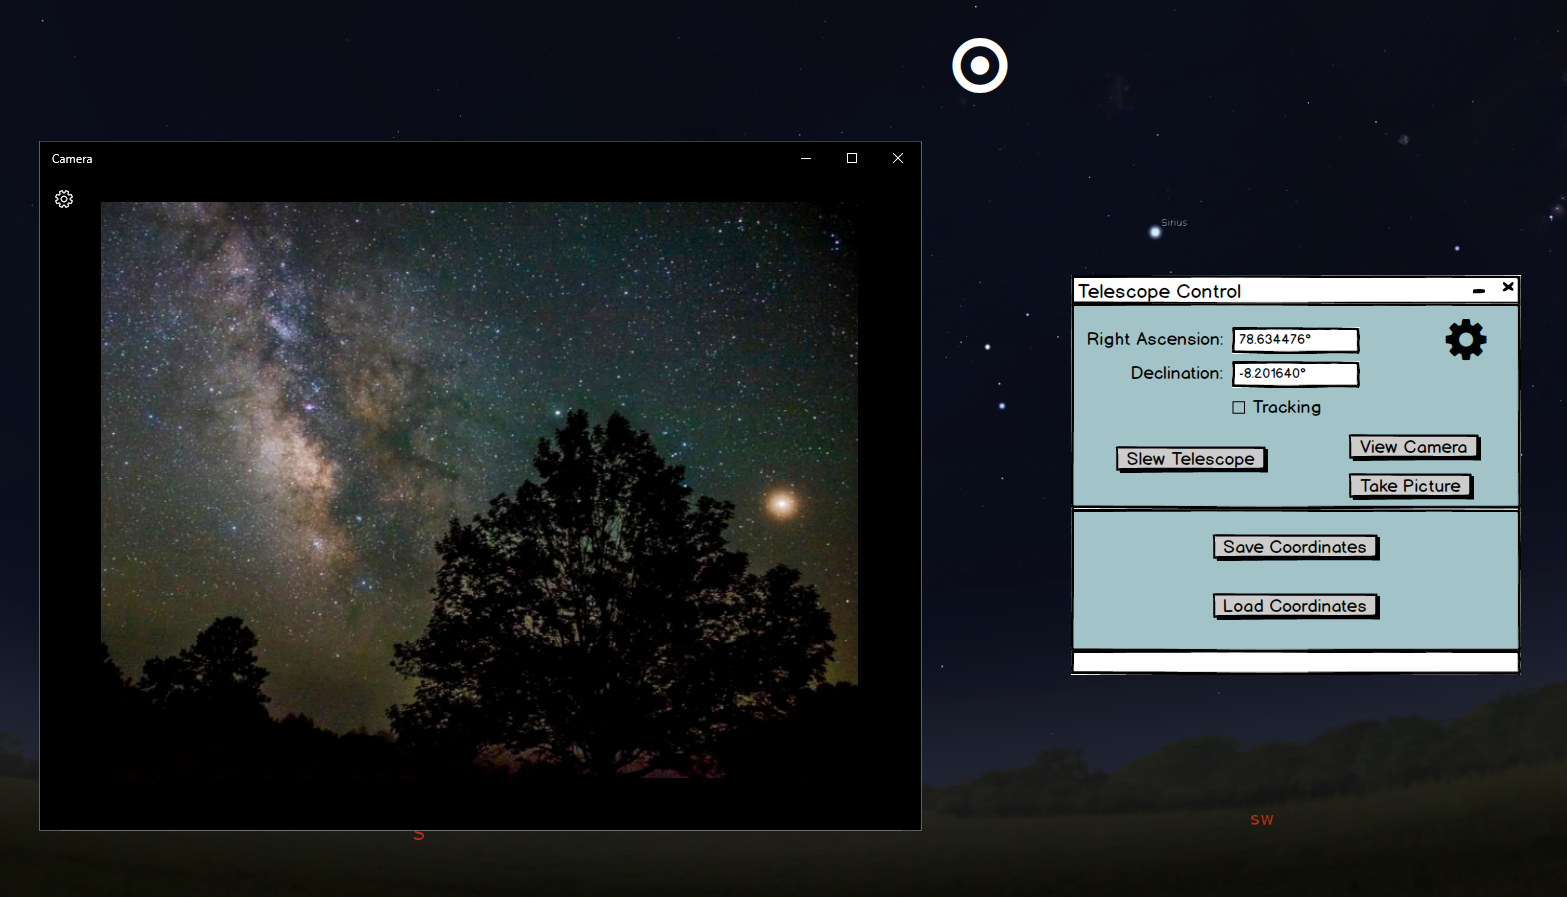
\includegraphics[width=0.90\linewidth]{MainScreenwithCameraView}
	\caption{Camera pop-up to view what the camera is currently seeing}
\end{figure}

The camera viewing application will be external of the control software, and will likely be the native camera software that comes with Windows. There will be warnings for when a camera is not detected when the user tries to use the camera options (Figure 3), or if there is no telescope detected when the user tries to move the telescope (Figure 4).

\begin{figure}[h]
	\centering
	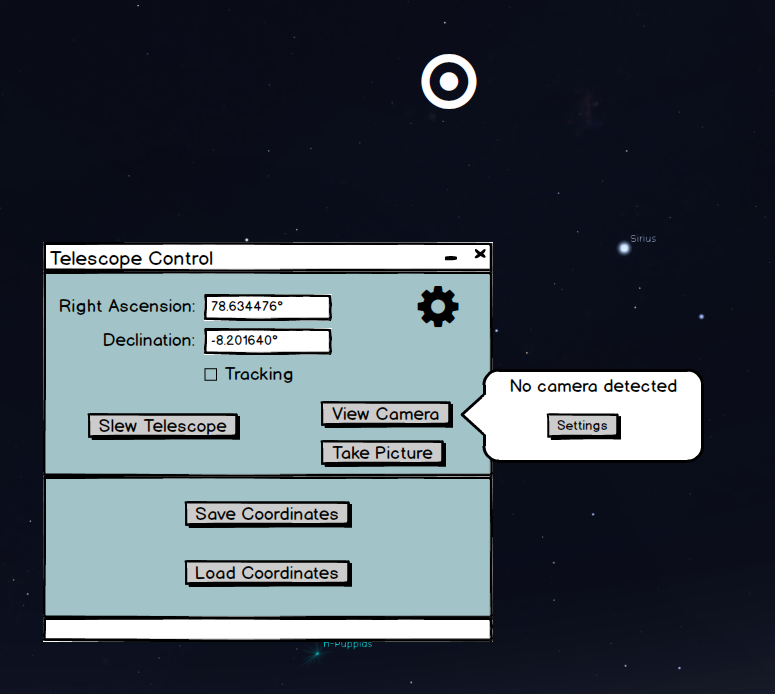
\includegraphics[width=0.70\linewidth, height=7cm]{NoCameraDetected}
	\caption{Warning that there is no camera detected}
\end{figure}

\newpage


\begin{figure}[h]
	\centering
	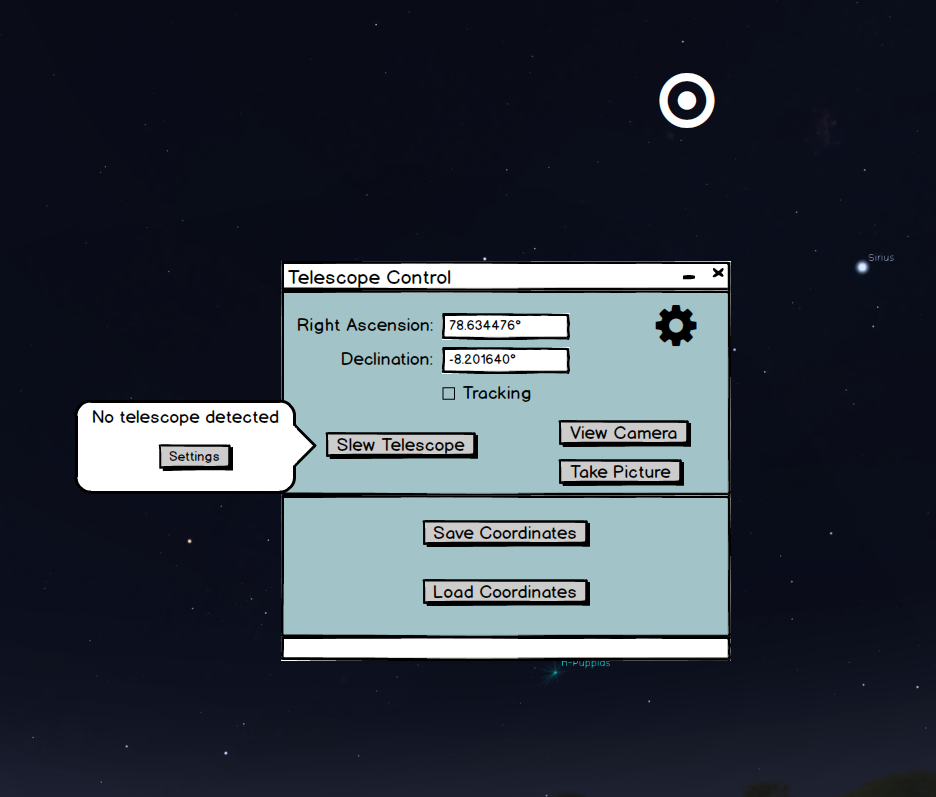
\includegraphics[width=0.70\linewidth, height=9cm]{MainScreenNoTelescope}
	\caption{Warning that there is no telescope detected}
\end{figure}

There will be fail-safes in place in case the user accidentally tries to move the telescope to an impossible position, as well as visual warnings as shown below (Figure 5). The user will have the option to override the warnings, but the telescope will stop when it reaches near a collision point, such as with the ground if the user is trying to look at a star that can currently only be soon on the opposite side of the world.

Another built-in fail-safe not necessarily shown to the user in the software is what is known as the 'Meridian Flip'. The Mechanical engineers that we are working with are designing the telescope to have a German equatorial mount. This is a type of telescope design that helps to track an object using constant speed movement on one axis that is oriented parallel to the Earth's axis of rotation. The downside to this mount is that the balancing arm, acting as a counterweight, can run into itself when tracking something that passes over the meridian line. Therefore, we will build a fail-safe that will do a 180 degree flip of the telescope when tracking across the meridian to avoid this collision.

Building this fail-safe into our software will also help further the understanding of how the Robinson Observatory's telescope works, due to it also having a German equatorial mount.

\newpage

\begin{figure}[h]
	\centering
	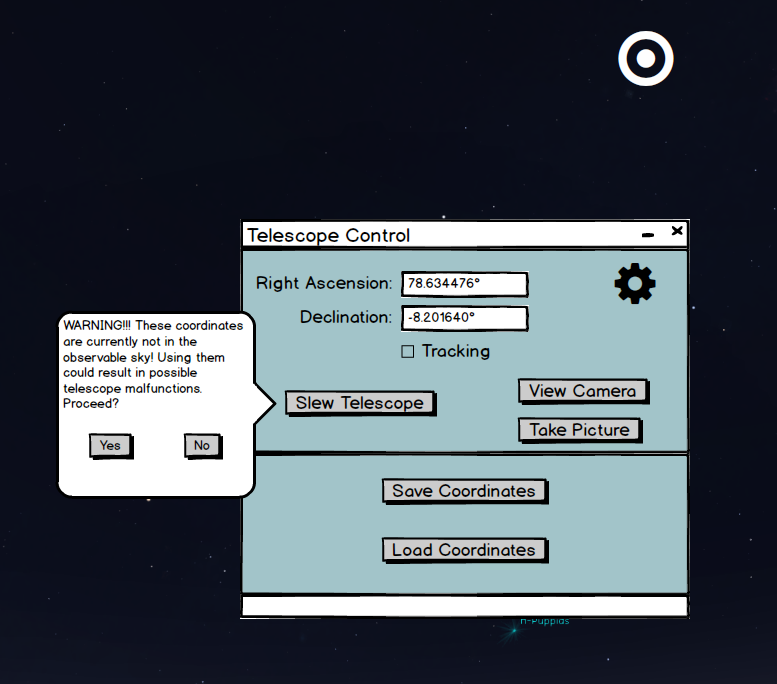
\includegraphics[width=0.80\linewidth, height=10cm]{MainScreenSlewWarning}
	\caption{Movement warning when attempting to move the telescope to an impossible position}
\end{figure}

Below these slew and camera options will finally be the saving and loading functionality as described in the next section.



\subsubsection*{Storing and Loading Previous Positions}

Other than movement, another focus of our software will be to store previous positions and movements as a list of searchable choices to then load into the telescope to move it without having to find that position manually in Stellarium's virtual planetarium again. This will be achieved by having the option to save your currently selected position along with a unique name and picture associated with the coordinates while the control console application is up and running (Figure 6). This can be done by clicking 'Save Coordinates' on the main page. Once saved, the position and chosen options are stored either locally or externally, or both, in the application to be searched for via a search user interface that can be accessed by clicking 'Load Coordinates' on the main page.

\newpage

This will also remember whether or not the user decided to track the position, as well as when this particular position was saved.


\begin{figure}[h]
	\centering
	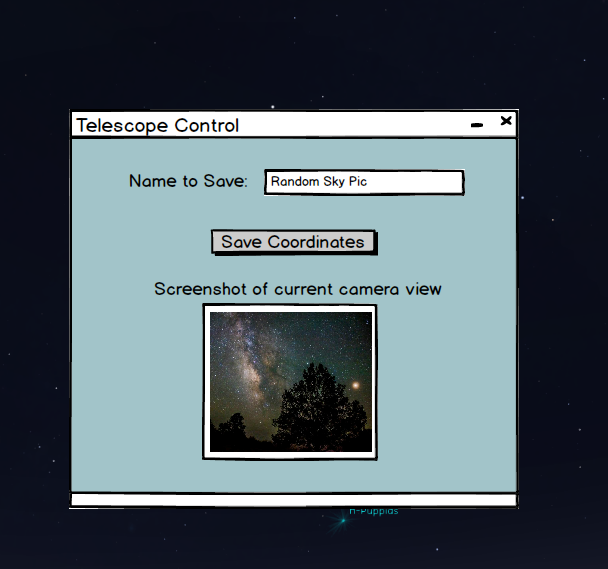
\includegraphics[width=0.60\linewidth, height=8cm]{Save}
	\caption{The save coordinates screen}
\end{figure}

This search page (Figure 7) will be dynamic in nature, searching through either both or separately files specified in a local save location and files stored in an external save location. These locations are edited in the settings, which will be further explained in the following section. As can be seen in the below figure, there will be four columns by which are self-explanatory within the figure. The unique column is the 'Picture' column, where a thumbnail of the picture related to that row's coordinate is shown. Clicking this thumbnail will cause a pop-up of the actual picture file (Figure 8).

This picture file will either be retrieved from local memory within our software, or from a user-specified external location as established in the settings. We will be implementing this into our website in a way such that the website will be able to draw form this exact same search list as the software is pulling from.

\begin{figure}[h]
	\centering
	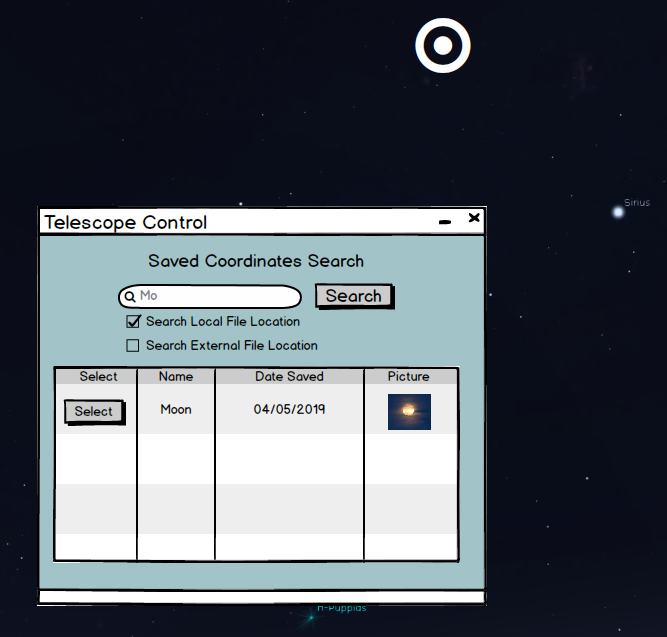
\includegraphics[width=0.55\linewidth, height=7.0cm]{SearchPage}
	\caption{The search page to load a previously saved coordinate}
\end{figure}

\newpage

\begin{figure}[h]
	\centering
	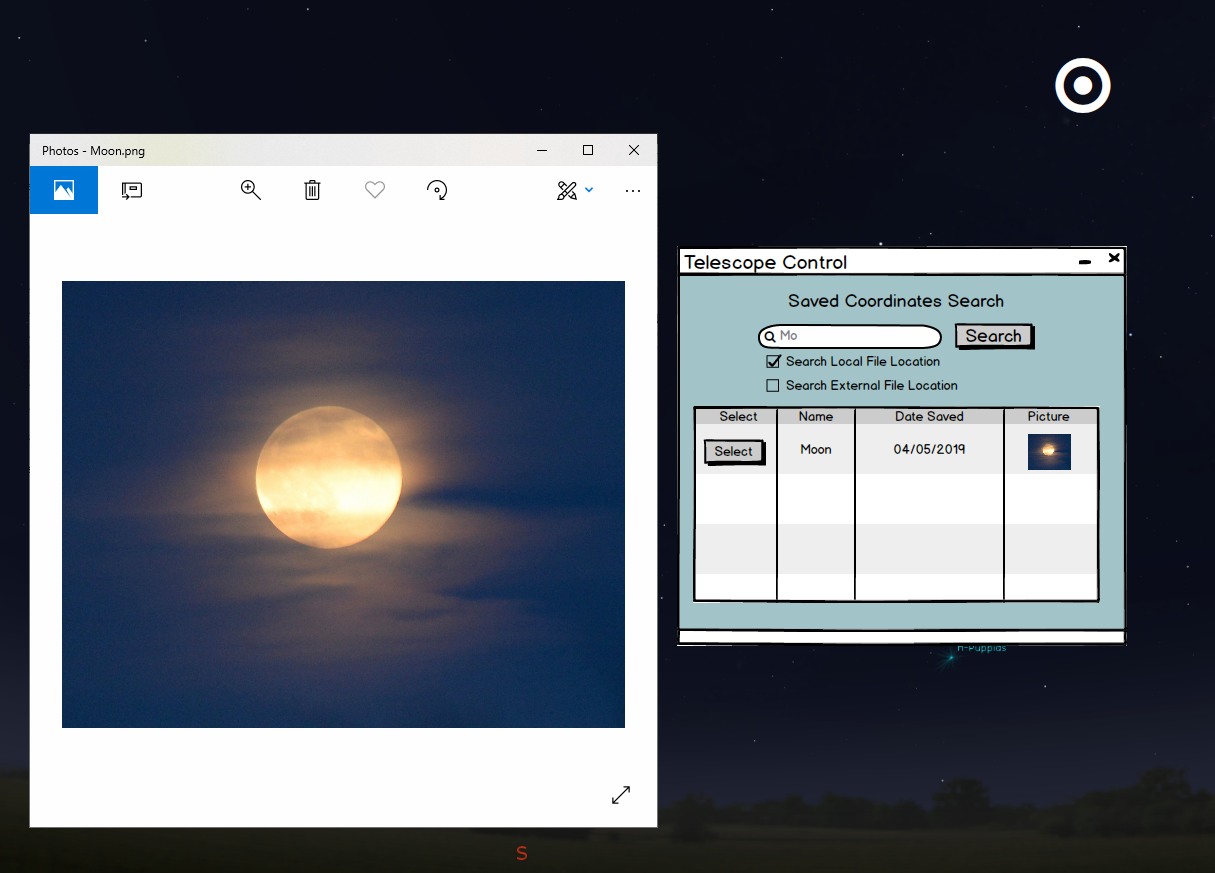
\includegraphics[width=0.65\linewidth, height=7.0cm]{SearchClickedPicture}
	\caption{By clicking the picture thumbnail, this will trigger the full-sized picture to pop up}
\end{figure}

The user can choose to load a given coordinate by clicking the select button on the chosen row, and this will bring the user back to the main page and will fill the coordinate textboxes with the saved coordinate information. However, we will have safeguards in place similar to the previously mentioned safe guards on the main page with moving the telescope. We will warn the user if they are attempting to load a coordinate that is currently not in the observable sky (Figure 9), because again this can cause possibly catastrophic issues.

\begin{figure}[h]
	\centering
	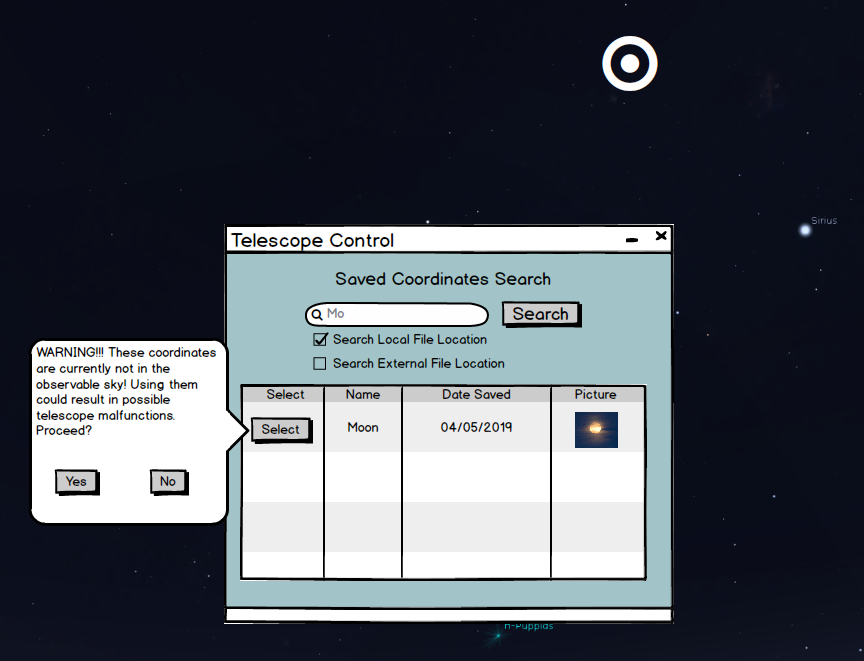
\includegraphics[width=0.65\linewidth, height=7.0cm]{SearchwithWarning}
	\caption{Warning triggered by impossible coordinates}
\end{figure}

\newpage

\subsubsection*{Setting the Settings}

The final main piece to our software is the settings page (Figure 10). This page is the customizable brains of the control software. On this page is where the user will choose from the list of detected cameras which one they would like to use as the main camera, as well as what type of format that the coordinates will have. The coordinates can have an hours-minutes-seconds, degrees-minutes-seconds, and decimal format.

\begin{figure}[h]
	\centering
	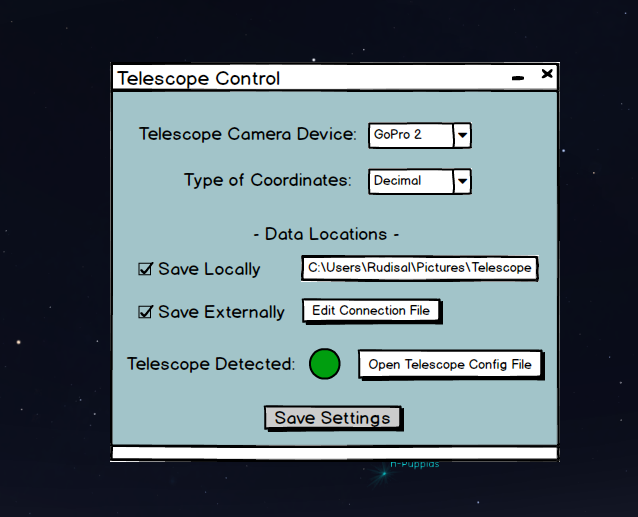
\includegraphics[width=0.75\linewidth, height=10.0cm]{Settings}
	\caption{The control software settings}
\end{figure}



Below those options is another set of options that we refer to as the 'Data Locations'. This is where the user will check whether they want to save their data that is getting stored and where that storing is happening, so long as they have one of the options checked. If both are left unchecked, then the software will assume that the user has no intention of saving any information. In terms of the 'Save Externally' option this is where the user can connect a service to the software that can take the pictures and information saved and put it on an external server, such as a website. For our project, we will set this up to communicate with the website that we are creating for the Robinson Observatory as explained later on in the paper. This 'Connection File' will require the user to have some knowledge in setting up server connections, but we will create the file with as many comments and explanations as necessary to facilitate an easy setup.

\newpage

The final part of the settings page, and arguably the most important part, is the actual telescope connection settings. Our software will be set up to automatically detect our custom telescope, but we will also create the connection file to be as easy to connect to any given telescope as we can possibly make it. There will be an indicator next to the setting that will either be green or red, dependent on whether or not a telescope is detected using the given configurated settings. Our projects main goal is to have this software work for our custom telescope, but a 'nice-to-have' goal would be to have this set up to easily connect any telescope. This will help facilitate the possibility of repairing the observatory, and could even possibly pave the way to implementing our software into actually controlling the observatory.


\subsubsection*{Software Creation Explanation}

As mentioned previously, we will be developing this console application in C++ using Visual Studio as our IDE. We intend on making this console application as a plug-in for Stellarium, and so therefore this software will only run accurately while Stellarium is up and running.

The process that we will go about creating this software is to first establish the math associated with converting equatorial coordinates into motor rotations. The core of the physical telescope is two motors run by an Arduino, one motor controlling horizontal movement and the other controlling vertical, and these motors will rotate a certain amount of degrees based on our math. This math is further explained in the math sections later on in this paper.

The next step will be integrating that math into our visual studio console application. Once it is integrated, it is then a matter of establishing the connection to the Arduino and sending the movement commands to the motors. These commands will simply be a string containing the degree of rotation for each motor, and the Ardunio will then issue the rotation commands to the motors themselves. The Arduino and motors are the responsibility of the Electrical team. This connection is what the 'Telescope Config File' entails in the settings page of the software, and it will be the process that acts as the go-between from our software to the motors, and vice versa.

We will then set up the auto-detection of any cameras connected to the system. We will use this auto detection to fire the camera application for the chosen camera, if one is chosen to begin with. The telescope is being designed initially to simply contain a high-grade laser to demonstrate it's accurate pointing and movement capabilities, and therefore our camera addition is not the highest priority.

Lastly, we will develop the file that will contain the information needed for our application to communicate to an external server whenever the user specifies external data locations. This will help facilitate our telescope communicating with our website.

\subsection*{ROS Integration with Stand-Alone Gazebo For a Testing Environment}

\subsubsection*{Explanation for Need}

This section will explain how we intent to test our software after it is created. As mentioned previously, we will be testing the software in a simulator environment before we use it on the physical telescope itself. The actual uses for this simulator environment, as well as how we installed and set it all up, is explained in the following sections.

\newpage

\subsubsection*{What is Ros?}

\begin{figure}[h]
	\centering
	
\includegraphics[width=0.50\linewidth]{melodic}
	\caption{ROS Melodic}
\end{figure}

The Robot Operating System, otherwise referred to as ROS, is a flexible framework used for the purposes of writing software for robotic systems. It is a collection of tools, libraries, and conventions that aim to simplify the task of creating complex and robust robot behavior across a wide variety of robotic platforms.\cite{ROSDescription} It is commonly used in conjunction with Python and C++, and for our purposes we will be programming in C++. Furthermore, ROS is home to a large community of user-contributed packages that adds a lot of value to integrating ROS into our core systems. Why reinvent the wheel and rediscover wood when we can instead invent a brand new cart from existing pieces already put together by other people for other projects?

The core of ROS is licensed under the standard three-clause BSD license. This is a very permissive open license that allows for reuse in commercial and closed source products. This works great for the purposes of our model telescope, because we wish to keep our creation entirely open-sourced. While the core parts of ROS are specified as being licensed under the BSD license, other licenses are commonly used in the user-contributed community packages such as the Apache 2.0 license, the GPL license, the MIT license, and even proprietary licenses. For the sake of our aforementioned open-source goal, our team will avoid any community packages that state the use of proprietary licenses. Every user-contributed package is required to explicitly state what kind of licensing it uses, and so this should not be an issue for our team.

\subsubsection*{What is Gazebo?}

\begin{figure}[h]
	\centering
	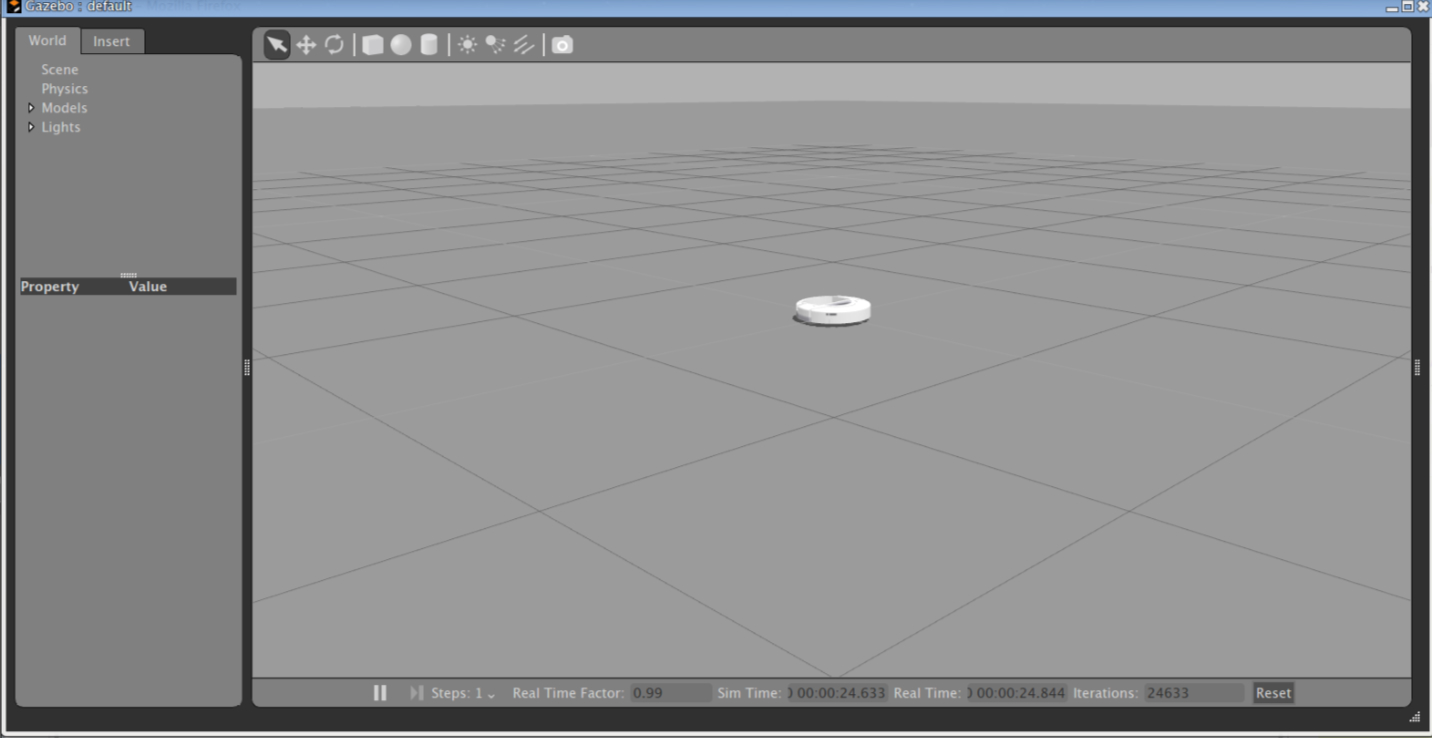
\includegraphics[width=0.98\linewidth]{gazebo}
	\caption{Example of Gazebo environment}
\end{figure}

Gazebo is a 3D dynamic simulator with the ability to accurately and efficiently simulate robotic systems in complex indoor and outdoor environments. While it appears to be similar to game engine environments, the differences in Gazebo lies in its ability to offer physics simulations at a much higher degree of fidelity, a suite of sensors, and interfaces for both users and programs.\cite{GazeboDescription} Other key features of Gazebo include multiple physics engines to choose from, a vast library of robotic models and environments, as well as advantageous programmatic and graphical interfaces. This will help create a more conductive programming environment for our team so that we can feel confident in what we create.

\newpage

Using Gazebo with our project gives us the ability to rapidly test algorithms in a simulation environment, design our model telescope with the understanding that it is a robot, perform regression testing, and possibly even train our model telescope to use a basic AI system that uses realistic scenarios. To accomplish all of this, Gazebo was designed to work on Linux operating systems and it works the best on Ubuntu, which is a flavor of Linux. Thus, this will require us to install Ubuntu in order to run Gazebo.

\subsubsection*{Ubuntu, a flavor of Linux}
To understand what Ubuntu is and how to install it, an individual first has to understand what Linux is. Linux is an operating system for a computer environment, and that means it is a software that manages all of the hardware resources associated with your computer. Linux is just another way to manage the communication between the software and hardware of your device.\cite{LinuxExplaination} The reasons behind why people use Linux are numerous, and the following are a few of the most common reasons:
\begin{description}[font=$\bullet$~\normalfont\scshape\color{red!50!black}]
	\item [Zero Cost of Entry] Linux is entirely free, and you can install it on as many systems as you would like without ever encountering a software license or fee.
	\item [Usability] You can do everything on Linux that you are used to doing on one of the more popular operating systems such as Windows or iOS. The key difference is that Linux has actually simplified many processes, and what can be a daunting task on one operating system is just a few commands and clicks on the Linux operating system. Hour long tasks can be accomplished in minutes.
	\item [System Administration] Linux is known as the "set it and forget it" operating system due to how it rarely changes it's core features, which means that you can be assured that once something is set up then you almost never have to worry about it again. Often times in other operating systems, key updates can break entire programs and cause the user to have to hunt down the issues and reconfigure multiple different areas. This is not the case with Linux, and even on the rare occasion that something within the operating system may break, almost always it does not affect any other part of the system other than the specific part that broke.
	\item [Open Source Licensing] Linux is also known as the operating system that is "by the people, and for the people". This is because Linux is entirely open-sourced and user-run, meaning that users have the freedom to run any programs for any purposes. They also have the freedom to redistribute any amount of copies as they wish, as well as modifying anything they would like and redistributing that as well. Linux is a virtual playground of options with almost no business-related consequences.
\end{description}

So then we come to the question of Ubuntu and what it has to do in relation to Linux. Linux has many different versions of itself, known as flavors, which goes hand in hand with what was stated earlier about freely modifying and redistributing Linux due to it's open-sourced nature. Ubuntu is a complete Linux operating system, and it is freely available to everyone with total support from both the community as well as professionals. The initial creators of Ubuntu created a manifesto when developing their flavor of Linux, and it's premise is that software should always be available free of charge and usable by people in their local language despite any disabilities, and that people should have the freedom to customize and alter their software in whatever way they see fit.\cite{Ubuntu} Ubuntu gets its professional support from Canonical Ltd, and Canonical's business model is to provide technical support and professional services related to Ubuntu free of charge now and always.

To now understand why both Gazebo and ROS use and take advantage of Ubuntu, we have to learn about one final puzzle piece, the Debian Project. Debian is an all-volunteer organization dedicated to developing free software and promoting the ideals of the Free Software community. \cite{Debian} Ubuntu and Debian are distinct systems but parallel in their endeavors, which makes them closely linked. One of Ubuntu's goals is to complement the Debian project. Many of Gazebo's packages are distributed using Debian systems, and so while working with Gazebo and ROS we will also be working closely with the Debian development community.

\subsubsection*{Installing Ubuntu}
While Unbuntu itself is an amazing piece of community-sourced software development, the actual installation of the operating system into a computer is another beast entirely. While it was designed to be as seamless as possible, the issues lie in the fact that most computers already have a standard operating system on them such as Windows or iOS. This brings us to one of two options, both of which are explained below:
\begin{description}[font=$\bullet$~\normalfont\scshape\color{red!50!black}]
	\item [Removing the current operating system and replacing it with Ubuntu] At the end of the day, operating systems are no more special than any other piece of software installed onto your device. Knowing this, it is simple to grasp that you can uninstall one operating system and replace it with another. This is a good option if you are not tied into your current operating system in any fashion, such as operating system specific software and programs that are essential to your needs, and if you are alright with switching to an entirely new type of operating system user interface and commands. It is highly recommended to have all of your information that you do not want to lose on a separate drive than what your operating system lives on, so that you do not run the risk of forever erasing any of that important data.
	\item [Installing Ubuntu beside the current operating sytem with dual-boot] You can also go the route of keeping your current operating system, and choosing to also install Ubuntu alongside it so that you can choose which operating system you will be working in on system startup. While this avoids the risks of having to untie yourself from operating system specific software, this introduces a whole new slew of risks due to this method messing with the boot manager of your motherboard's Bios and other such activities. Motherboards, the brains that control our computers, do not have built-in methods of running between two separate operating systems. Therefore, part of the Ubuntu dual-boot install requires the installing of a custom boot-up user interface, known as GRUB, that will let the user pick which operating system to use.
\end{description}

For the sake of our development, we went the dual-boot method so that we can maintain our current system environments while also having the ability to switch to Ubuntu for the sake of our project development. In order to begin this method we first have to create a bootable USB drive with Ubuntu installed on it so that our computer can boot into that drive. To create this bootable USB drive we needed a USB writing tool, and so we went with Rufus which is a widely-used open-sourced tool for writing ISO files onto flash drives. Having installed Rufus, as well as downloading the latest version of Ubuntu from Ubuntu's official website, we then use Rufus to make our flash drive a bootable Ubuntu USB (Figure 13).





\begin{figure}[h]
	\centering
	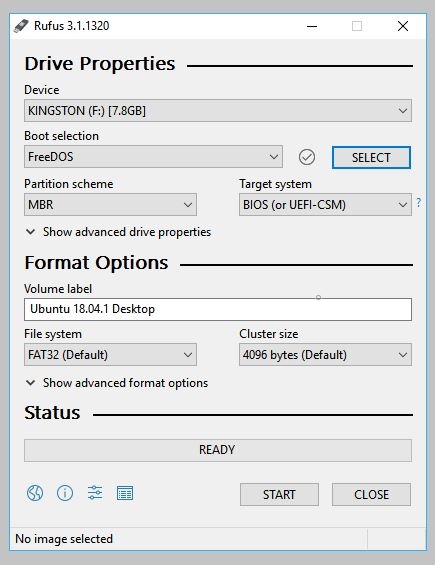
\includegraphics[width=0.50\linewidth]{rufus}
	\caption{Rufus}
\end{figure}

Once this is done, we powered down the computer and turned it back on. When first turning on, we switch the initial boot device from our normal operating system to the USB that we plugged in. This will then boot into Ubuntu where we are presented with the options to install (Figure 14). Choosing the dual-boot option on the next page will bring us through some various choices screens and account setup, and then we hit the actual installation (Figure 15). Once installed, we can now dual boot into either of our operating systems using the new GRUB menu (Figure 16).

We then have to actually set up our working environment within Ubuntu. This involves installing ROS and Gazebo and getting them up and running on our machine. The following sections will cover how to do exactly that.

\newpage

\begin{figure}[h]
	\centering
	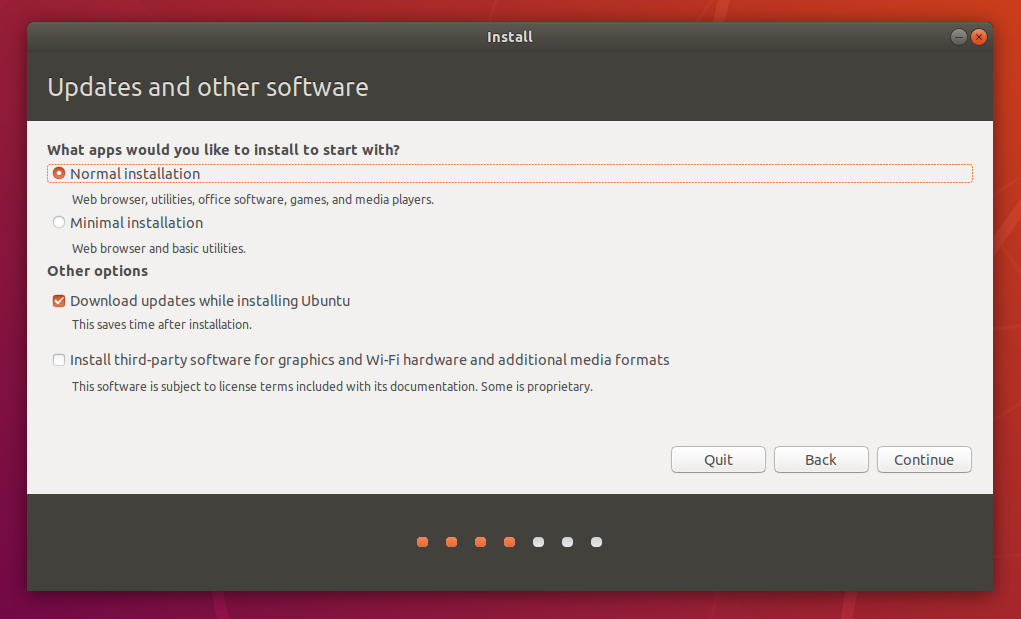
\includegraphics[width=0.50\linewidth]{install}
	\caption{Ubuntu Install Options}
\end{figure}

\begin{figure}[h]
	\centering
	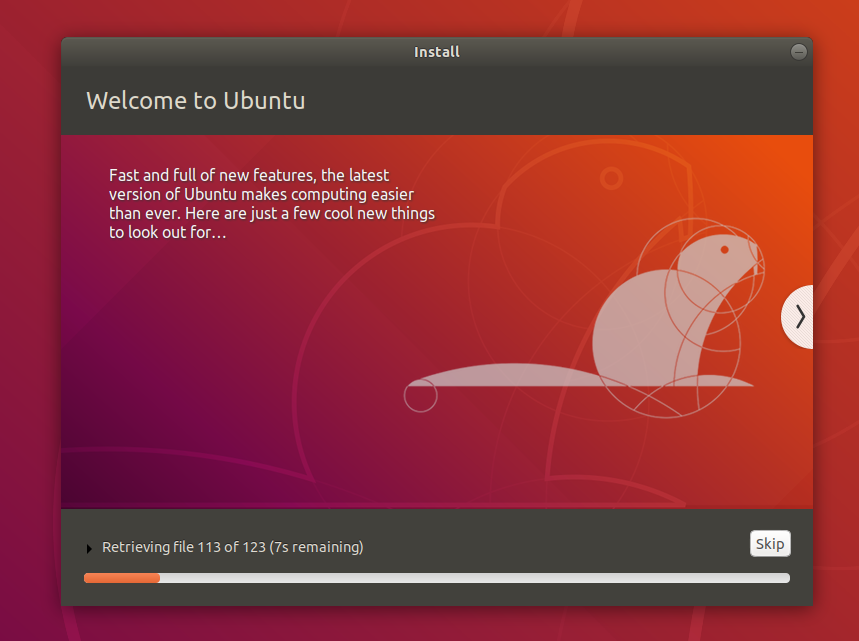
\includegraphics[width=0.50\linewidth]{installing}
	\caption{Ubuntu Installing}
\end{figure}

\begin{figure}[h]
	\centering
	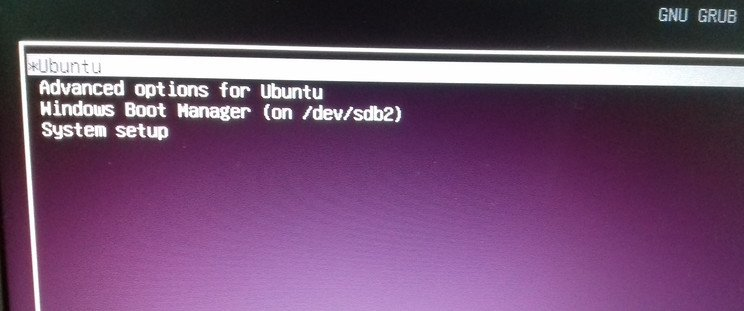
\includegraphics[width=0.42\linewidth]{dual}
	\caption{Dual-booting}
\end{figure}

\newpage

\subsubsection*{Installing Gazebo}
\indent Using Ubuntu packages, installing Gazebo is just a few simple steps. First we had to set up our computer to be able to accept software packages from 'packages.osrfoundation.org' by running the following command in the terminal:
\begin{verbatim}
sudo sh -c 'echo "deb http://packages.osrfoundation.org/gazebo/ubuntu
`lsb_release -cs` main" > /etc/apt/sources.list.d/gazebo-latest.list'
\end{verbatim}

We then have to setup the keys and install Gazebo itself with the following terminal commands:
\begin{verbatim}
wget http://packages.osrfoundation.org/gazebo.key -O - | sudo apt-key add -
sudo apt-get update
sudo apt-get install gazebo5
\end{verbatim}

That's it! Gazebo is successfully installed, and we cna check this by running the 'Gazebo' command on the terminal window.

\subsubsection*{Installing ROS}

Installing ROS is an extremely similar process to installing Gazebo. In fact, that's an example of what was stated earlier about why Linux is so straightforward ot use! First we had to set up our computer to be able to accept software packages from 'packages.ros.org' by running the following command in the terminal:

\begin{verbatim}
sudo sh -c 'echo "deb http://packages.ros.org/ros/ubuntu $(lsb_release -sc)
main" > /etc/apt/sources.list.d/ros-latest.list'
\end{verbatim}

We then have to setup the keys and install with the following terminal commands:

\begin{verbatim}
sudo apt-key adv --keyserver hkp://ha.pool.sks-keyservers.net:80 --recv-key
421C365BD9FF1F717815A3895523BAEEB01FA116
sudo apt update
sudo apt install ros-melodic-desktop-full
sudo rosdep init
rosdep update
sudo apt install python-rosinstall python-rosinstall-generator python-wstool build-essential
\end{verbatim}

There you have it, a full install of ROS. Now comes the final piece, which is integrating ROS with Gazebo. To successfully achieve a ROS integration with stand-alone Gazebo, a set of ROS packages named "gazebo ros pkgs" provided by Gazebo, provides wrappers around the stand-alone version of Gazebo.\cite{GazeboRosIntegration} They provide the necessary interfaces to simulate a robot in Gazebo using ROS messages, services and dynamic reconfiguration.


\subsubsection*{Summarizing the Simulator Environment}

Now that we have the test environment fully set up and ready to be used, we now have a firm foundation to ensure that the model telescope will function by the time we have to present it. This simulation environment can, and will, be used by all of the teams by integrating every teams components together to demonstrate a working model before any physical pieces are even put together. This will make testing and debugging extremely less taxing on all of us and will ensure that we can accurately predict as many different user situations as the simulator can make so that we can plan for every eventuality.

We plan on relying heavily on this simulator throughout senior design 2 so that we can troubleshoot issues seem when the physical telescope is not obtainable in that moment.

\subsection*{Control Software Options}

The interdisciplinary part of this project deals focuses on the creation of a sub-scale model similar to the Robinson observatory telescope. In order for this telescope to move, we need to either find a suitable open-source software to use, create our own telescope control software, or combine a mix of both. Currently, the observatory uses SkyX Professional as it is the software provided with the Paramount telescope they purchased. The software provides control outputs to a black box on the telescope, which then sends movement operations to the gears. When the telescope was functioning properly, the software worked well for those controlling the telescope. The problem now is the telescope is not in a properly functioning state and the exact reason can’t be determined. The software gives multiple error messages when in use but it can’t be determined in the software is no longer properly parsing the data because of a modifications to the settings or mechanical issues. With the connection to the black box, which is provided by Bisque, the cycle of information is currently unaccessible due to lack of information. There is no documentation on the black box so it is unknown how the black box parses input given by the software and creates gear movements. In order to properly dissect this box, the time needed would take too long for the scope of this project. This is only on reason we must find a new software.

The other reason we are looking for a new software is SkyX Professional used for observatory control is placed behind a paywall. SkyX does have a free version but this versions purpose is to help teach the user on space not provide telescope control. The professional version can be bought for \$329.00 on www.bisque.com. While this is a steep price to pay, we could find a way to help pay for this cost as a Senior Design project. The issue the paywall brings up is limiting the community outreach our project could have with an open source program. SkyX and its price tag could cause many people to not use our project for themselves. So with the combination of the needed black box and the price tag, we want to pursue other options. Options that are easily accessible for everyone to provide a functioning telescope control program.

Since we will not being using the SkyX software, we need to find an option that mimics many of SkyX’s core features to make a transition easier if the observatory finds they would prefer our program more. At the beginning of this project when we were tasked with repairing the observatory telescope, the faculty working at the observatory were atimitment about keeping the SkyX software. We would like to show another option for telescope control while providing the observatory with the functionality they like. With SkyX being a paid software, it is more polished and refined compared to open source programs. This does not translate into a head and shoulders better program though.

An important aspect our software will not replicate is the control of the dome at the observatory. With SkyX, the observatory is able to directly connect the control of the dome with SkyX. The dome protects the telescope and only has a small portion the telescope can see out of. When tracking an object, the dome moves along with the telescope to ensure the telescope still has a clear view of the sky. Our sub-scale model will not feature a dome and furthermore, the open source programs available do not allow for the direct connection like SkyX does.

The software chosen will send information between an Arduino board. This board will connect all the functioning pieces of the telescope together. The board is programmed in C with a plethora of libraries available to use and will be developed through both us, the Computer Science team, and the Electrical engineering team. Our job will be providing the EE team with motor movement commands, either through inputs to the board or through functions within the Arduino software. These options depend on how the telescope software sends information.

If we chose open-source software, the only modifications that would need to be made are for the formulation of gear/motor movements for the telescope. So the selection of open-source software should be based on the interface the software provides. Is it easy to select where the telescope needs to point? If it is a better idea to calculate these movements in the Arduino software, the telescope software will not require modifications. There are multiple options for the telescope software that will be reviewed in the following paragraphs.

\subsubsection*{Technical Overview}

The objective of our software development for telescope control is to provide a functioning program that allows a user to pick a point in the sky they wish the telescope to point at on the Windows platform. From there, the program will relay this position in either location strings or motor movements to our telescope for proper repositioning. Our program should also house the ability to track an object like the Sun or Moon. This requires the constant relay of instructions to the telescope. These base functions are the requirements for the program and can be tested through the images captured by the camera attached to the telescope. A stretch goal on top of these requirements is provide a way of tracking a faster moving object in the sky. This goal is more of a shared goal between the teams of this project as the telescope needs the proper movements associated to the output given by the control program.

The goal for the software development is provide a simple and easy to use interface for telescope control for beginners, experts, and everyone in between. The program should provide telescope control with simple setup for the whole range of users. The only modifications needed should be adjusting motor commands to the specific motors/gears used. Furthermore, our program should be similar in function to SkyX to help provide a well-documented project showing the general flow the observatory telescope would take. We want to show the control process can be completed without SkyX while still performing to the same standard the observatory had come to expect. The documentation created from this project could also lead to insight in where the current observatory telescope process is failing.

\begin{figure}[h]
	\centering
	\caption{Overview of Control Communications}
	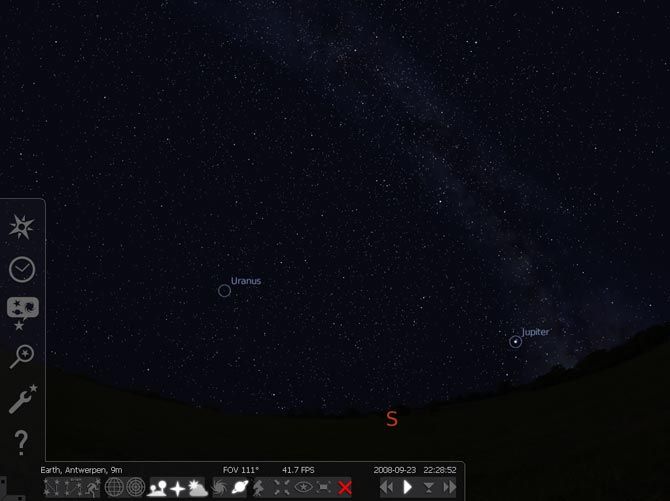
\includegraphics[width=1.0]{stell}
\end{figure}

\subsubsection*{Stellarium}

Stellarium is the first open source program we came across. Stellarium was a project started back in 2001 by Fabien Chéreau (“Stellarium Astronomy Software.”). The software was first released in July of 2014 and had its most recent update in December of 2018. Each of its releases can be found on their GitHub repository with a change-log. The software can run on Linux, Windows, or Mac so no compatibility issues will arise.

\begin{figure}[h]
	\centering
	\caption{Stellarium main page}
	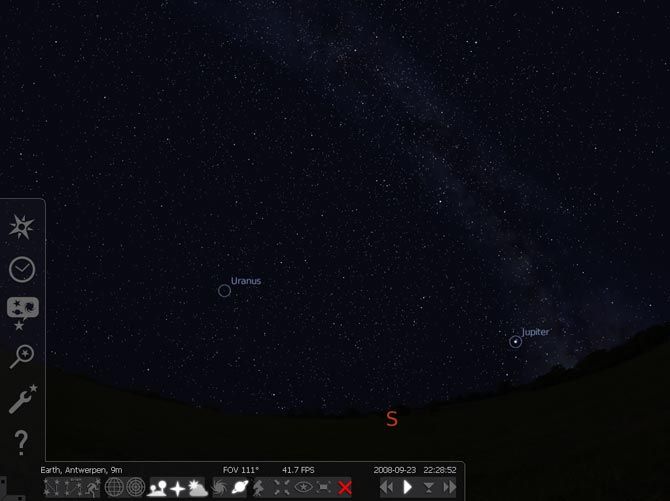
\includegraphics[width=1.0]{stell}
\end{figure}

Stellarium at its core is used to show a 3D model of a realistic sky. You tell the software what you want to view and it creates a visual 3d output of the sky at that location. It is not a current view of that location. For this project though, we would need to push beyond this core use and use their telescope control feature that was implemented in version 0.10.5. The software plugin allows you to control a GOTO telescope from the Stellarium UI through some basic instructions. This feature sends movement commands to the telescope and receives the current position of the telescope. By no means does the plugin allow for broad control of a telescope like SkyX does, the software does provide the functionality we are looking for. Supervision will need to happen during telescope control though as warnings for slew commands are not currently implemented by Stellarium. The issue that arises is when a slew command has the inverse effect of causing the telescope to hit itself. The software does not know the limitation of the telescope so it always assumes the telescope can be slewed to any position. It is also important to note the telescope can end up being pointed at the Sun, which is dangerous to view at without the proper filters on a camera that is mounted on our model.

With Stellarium, the telescope control feature works in two ways: direct or indirect connection. Direct connection will send slew commands and positional coordinates of the model through LX200 protocol. This protocol sends two strings for slew commands: one relates to right ascension and the other relates to declination. Depending on the type of mount used for the model, it may cause the need for conversions in coordinate systems. Stellarium only sends equatorial coordinates. These coordinates are a standard used by astronomers as it doesn't require constant recalculation. The current observatory uses an equatorial mount so it also deals with equatorial coordinates. If the sub-scale model follows this mount, no conversions need to be made. However, if an altazimuth mount is used, conversions will need to be made in the Arduino software from equatorial to the altazimuth coordinate plane. Thus, it would be in the best interest of this computer science team to follow the current observatory mount into the sub-scale model.

\subsubsection*{Cartes du Ciel / SkyChart}

The next option available is Cartes du Ciel written by Patrick Chevalley (Chevalley). SkyChart's base use, like the name implies, is draw sky charts. A sky chart is similar to a map as it shows the location of stars in the current sky. This software is open-source and available on Windows, Mac, or Linux. Since this software is based in the drawing of SkyCharts, its open library has a plethora of information. People can upload their charts to the library for others to use. This mass database is useful for stargazing on specific stars and space areas, something our model will not need to feature. Our model will not have the camera range to prove if we are looking in the correct area for many of the charts available. This would be a great feature for the observatory though, as it has a camera strong enough for detailed viewings of space.

\begin{figure}[h]
	\centering
	\caption{Carte du Ciel main page}
	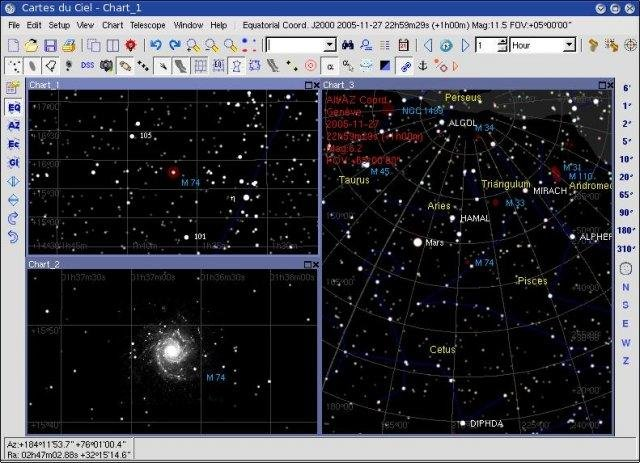
\includegraphics[width=1.0]{carte}
\end{figure}

Through the use of these charts, the software provides a vast library of objects to choose to slew a telescope to. To do so, the software can talk through the LX200 protocol like Stellarium. Furthermore, it supports INDI protocol for Mac and Linux while supporting ASCOM protocol for Windows. The ASCOM and INDI protocols are used to bridge the connection between control software and telescope. They are both open source frameworks designed specifically for the astronomy field. These protocols work through middleware causing the need for more software to be involved. The simplest option would to use the LX200 protocol to keep all operations within the software.

SkyChart adds more options for how to send data between the software and our telescope. These protocol options would be more helpful though with the observatory telescope. The sub-scale model will be very simplistic in features. We do not need to worry about camera focus or dome control like the observatory does. These features would find use with the INDI and ASCOM protocols as you can send more information between telescope and software. As we only need slew commands and position strings, the LX200 protocol is still most useful for the model.

\subsubsection*{Modifications needed}

Stellarium and Cartes du Ciel are both viable solutions providing us with telescope control. Yet, the output they produce would not be readily available for the Electrical engineering team since both softwares output coordinates for each motor as a string. In both instances, we need coordinate conversions to motor instructions and the calculation of the meridian flip. This flip is needed because of the use of the german equatorial mount. When the telescope is tracking an object trough the sky that passes the meridian, the telescope would run into its own mount. To stop this from happening, at the meridian, we need a recalculation for the location that includes reversing the orientation of the telescope. Once flipped, the telescope can proceed tracking to the East.

These modifications can be attacked two ways. The first option is programming the needed calculations in the Arduino software after being provided the command from the software. The other option is developing a new software to manipulate the strings outputted by the open source program. If we make all changes on the Arduino board, it allows us to segregate all specific motor instructions to the board instead of trying to modify the source code of a program. Even though documentation is provided with the open source programs, we could end up altering some state within the program that should not be changed. An example would be deleting some function you think is no longer needed yet when you run the new version, the program no longer runs.

\subsubsection*{Personally Developed Software}

The creation of a new software would provide us the opportunity to develop controls specifically for our telescope. Furthermore, it would take some processing power needed for motor movement calculations off the Arduino board and onto a computer. Finally, this new software could be written in the programming language of our choice and the ability to develop around Gazebo allowing for easy testing.

We can still develop software without creating a new planetarium program. The great thing about open-source software, besides it being free to use, is the ability to modify the software so long as we provide our developed software as open-source too. This software can use some of the features from the open-source programs like the vast knowledge of locations of stars in the sky held in Stellarium and SkyCharts.

Personally developing software a new program or even just modifying existing source code for our telescope may hurt the community outreach available. A hope of the model is that people can follow our instructions and software to create their own telescope. Some users may not have the same motors as us though. With our own software, the point of development would be to customize a program to our specific telescope. This may create areas where we are hard coding specifications of our telescope into the source code of the program. This could make the software unusable for others if they don’t build the telescope to our specifications. This may be avoidable by ensuring all telescope specific operations are handled by the Arduino but may also be unavoidable. Another possibility to maintain our outreach is providing detailed instructions on how to alter the code we create to suit the motor capabilities of the user at hand. Some people would not want to alter source code though for reasons of inexperience or not feeling comfortable. Another possibility to offset this possible negative consequence is providing the user with a telescope motor configuration option when connecting their telescope. The user would just input the specifications of the motor and gear setup they have. The software would then use this information to calculate the proper movements of the their specific telescope. This solution provides the broadest positive impact to our outreach but may produce issues we are unaware of. Our main goal is to provide our sub-scale model with a properly functioning control software. If we become stuck on an issue of compatibility with other telescope configurations, we could hurt the functionality of our telescope.

\subsubsection*{Comparing Options}

Our options come down to two prior developed programs or developing our own. As we are more focused on the controlling the telescope than just a planetarium program, we should stick to prior developed programs. These programs already provide the mapping of stars needed to provide the correct slew strings to our telescope so there is no need to build a program from scratch.

Next our concern shifts to user experience. To help choose the best option, we can look at the process of telescope control in both programs and decide what provides the best way. Stellarium provides a minimalist viewing screen where most menus are hidden until you drag your mouse over the menu. These two menus that help provide most of the functionality are on the left side toward the bottom and at the bottom toward the left side. Then when a valid object is chosen in the sky, details that cover most of the left side of the screen pop up. SkyCharts also provides information on a selected object in the same fashion but with much less information compared to Stellarium. Stellarium provides a long list of the object in different coordinates like equatorial, cartesian, and galactic. Most of the information many people would not care about but nonetheless its provided.

With SkyCharts, you are presented with a screen much like an old version of Windows Office. The top portion of the screen is dedicated to a ribbon bar. On this bar, you are provided with all the functionality SkyCharts provide. Some options are buttons that turn on or off some feature while other options open up a pull down menu. SkyCharts does allow for multiple charts to be open in the same screen. This is a nice feature when looking for a star or planning out a future telescope control but would not be used too often for our purpose. For the user, Stellarium provides a cleaner look. You are not overwhelmed by the plethora of options that SkyCharts shows you while still providing most of those options. This can make it more difficult for someone to find an option in Stellarium over SkyCharts though.

Finally, some small features for each that are useful for development. Both programs are still being updated constantly to fix bugs and help keep the programs up to date with the current OS versions of the time. Stellarium uses GitHub to house their source code, which is convenient and provides and plethora of information including change logs and documentation. SkyCharts does not have a GitHub repository link and rather links to www.sourceforge.net to download the source files. SkyCharts still provides a documentation on their official site for all details relating to SkyCharts where items like change logs and a roadmap for future versions can be found.

\subsubsection*{Challenges}

The first challenge, and most likely the biggest, will be relating software commands to telescope movements. As a computer scientist, we mostly live our lives in a virtual realm. However, this project is breaking that barrier. Our software development will have a direct impact on the movement of the model telescope. We need to find a way to turn location strings into proper movements based on our specific functionality of the telescope. With our telescope being designed from the ground up, the gear ratios and motor torque will be unique. So, the Arduino board will not be able to directly execute the strings given by the software we choose. We will need calculate conversions for the coordinates given by Stellarium as well as formulating a meridian flip. Luckily, I have taken some mechanical engineering courses that have dealt with these topics giving me confidence when tackling these issues. I also have a minor in mathematics to help us through the conversion processes. The problem not only lies within conversions but also coordinating with the electrical team of how they want the strings to be presented. We need to ensure we are in constant communication with them throughout this process so neither team ends up with unusable code.

The next challenge is reviewing the current code of Stellarium to find the areas where we will place in our modifications. Currently, most of the telescope control program does not feature documentation informing you of what the current function is accomplishing. Thus, we will need to take the extra time of reading through the plethora of code so we can pin point the areas we want to modify. When trying to decipher code, the easiest path is talking to the writers of this code. As this is not always possible no matter where your project is occurring, personal or work life, this will be good practice for the team.

Furthermore, a challenge we face is testing. How will we know whether our software is correctly controlling a telescope while our sub-scale model is being built? This is where we will use Gazebo. Ideally, our control plugin we create will be able to work in Gazebo where it will control a robot until the model is built. Once the model is built, testing will be handled through tracking objects with a GoPro and/or laser pointer. The GoPro can show success or failure in tracking objects through video. A laser pointer can show proper movement to a set coordinate and even tracking but someone would need to constantly be checking the accuracy of the laser to the object. Can we control the telescope to track the moon or sun? This will be our big test on the system as a whole. Testing is also not just important to ensure we can control a telescope but also are our coordinate conversions correct. Yes, math conversions can be checked on paper but what if we are missing an important step between motor instructions and celestial coordinates. This issue arises from the time dependency of celestial coordinates and the inactivity of the telescope between uses. When dealing with this kind of issue, it can usually be troubleshooted through trial and error. The problem is the design of the telescope has not been finalized as of yet so we cannot put our conversions through a process of trial and error since we don’t know gear ratios and stepper counts for the motors.


\subsection*{Software design overview}

After research into open source programs, our group has decided with using Stellarium as the frontend software control program. We will then add onto to Stellarium’s code to create the needed strings the EE team needs in their Arduino board. The EE team is looking to receive information containing which motors need to move, the direction needed to move and how far the motor needs to move. These calculations will be made before we send any information to the Arduino board through USB. After the movement is complete, our software will receive a string informing us if the movement was successful or not.

The choice for Stellarium was a combination of popularity and a simpler user interface. An interface that is not as jumbled as SkyCharts, which could lead to confusion with inexperienced users. Since both programs offer an extensive library for object coordinates and provide telescope control through the LX200 protocol, the decision came down to simplicity. Stellarium offers an easier to use interface in our opinion and through research seems to be the choice made by many for an open source control program. Finally we decided to use an open source program instead of creating our own so we can focus strictly on the instructions we will be giving to the Arduino board. Stellarium provides everything and is in a stable working condition. Thus, there is no need to develop our own planetarium program when we are only interested in telescope control. The modifications will be made in the plugins section of the Stellarium code. All telescope control features are housed within the plugins section for telescope control. These files are written in C++ and include header files as well.

We want to still modify the telescope control plugin provided because we believe there is a better way of handling control we need than Stellarium does. The control plugin lacks instructions and can be hard to find unless. In the source code, you can find simple instructions for use commented within the code. We also want to add more features to the telescope control plugin to be discussed in further detail in the accompanying sections.

\subsection*{Modifying Stellarium}

To convert the output strings sent by Stellarium for the telescope control, modifications will be made to the telescope control plugin. This plugin can be easily found within the directory for plugins in the Stellarium source code. All code pertaining to telescope control is written in C++, which can be edited with nearly any text editor. Our edits will be done within an integrated development environment (IDE) though. An IDE like Visual Studio Code allows us to view errors within our modifications before compiling the software as a whole. We plan to only modify code pertaining to the LX200 coordinate output along with the windows created for telescope control. We will only modify LX200 outputs as this is the protocol we will use. There is no need to alter other protocols we are not familiar with and possibly break those protocols within Stellarium. Next, we will modify the control windows to add features like saving coordinates and viewing the live stream of the GoPro on the telescope. We also want to add more text within the windows to help provide a greater walkthrough of the telescope control process. This would allow a user to simply follow the onscreen instructions when setting up and using the telescope control instead of reading through documentation as many people don’t read the documentation anyway. A user friendly approach instead of simply creating the telescope modifications needed ensures for a pleasant using experience. An experience that could make the difference between wanting to use our software or looking for a different option.

\subsection*{Compiling Stellarium}

Since Stellarium is open source, the source code is obtainable online but the program can be installed straight from www.stellarium.org. In our case, we want the source code version so we can manipulate some of the outputs of Stellarium. In order to compile the code after modifications, QT5, CMake, and Visual Studios 2017 are all need to be downloaded. As a side note, Visual Studios 2017 is a minimum requirement. You can use a more recent version but this process is guaranteed to work with that version. All these downloads are available online as open source options. The community edition of Visual Studios works for this process. The source code can be obtained through git requests in a terminal, downloaded online, or through GitHub Desktop. If using Github Desktop, after cloning the repository, you should not be sending your modification back to the Stellarium repository.

To compile the code, Qt5 is first used to configure debug and release builds. When using Qt5, it is important to match the version of Visual Studios to the appropriate Qt5 version as the IDE within Qt5 depends on Visual Studios. Next, CMake is used to configure some user options onto the build. It is recommended to use version 3.4.1 or better. Finally, Visual Studios is used to change the build mode to release and build the program. This process can be started in one of two ways: by executing this file, C:\\Devel\\stellarium\\builds\\msvc2017\\Stellarium.sln, or by clicking the open project button from the CMake GUI. After this process is completed, the program has been complied and is thus ready to be used.

\subsection{Using Stellarium}

First Time Use Setup - The telescope needs to be configured within Stellarium.
	1. The telescope will be connected through USB. Once plugged in, ensure Stellarium recognizes the connection.
  2. Press F2 to open the configuration settings window.
  3. Select “Plugins” from the tabs available.
  4. Select “Telescope Control” from the options on left (image above shows telescope control plugin page).

\begin{figure}[h]
	\centering
	\caption{Stellarium Telescope Control Window}
	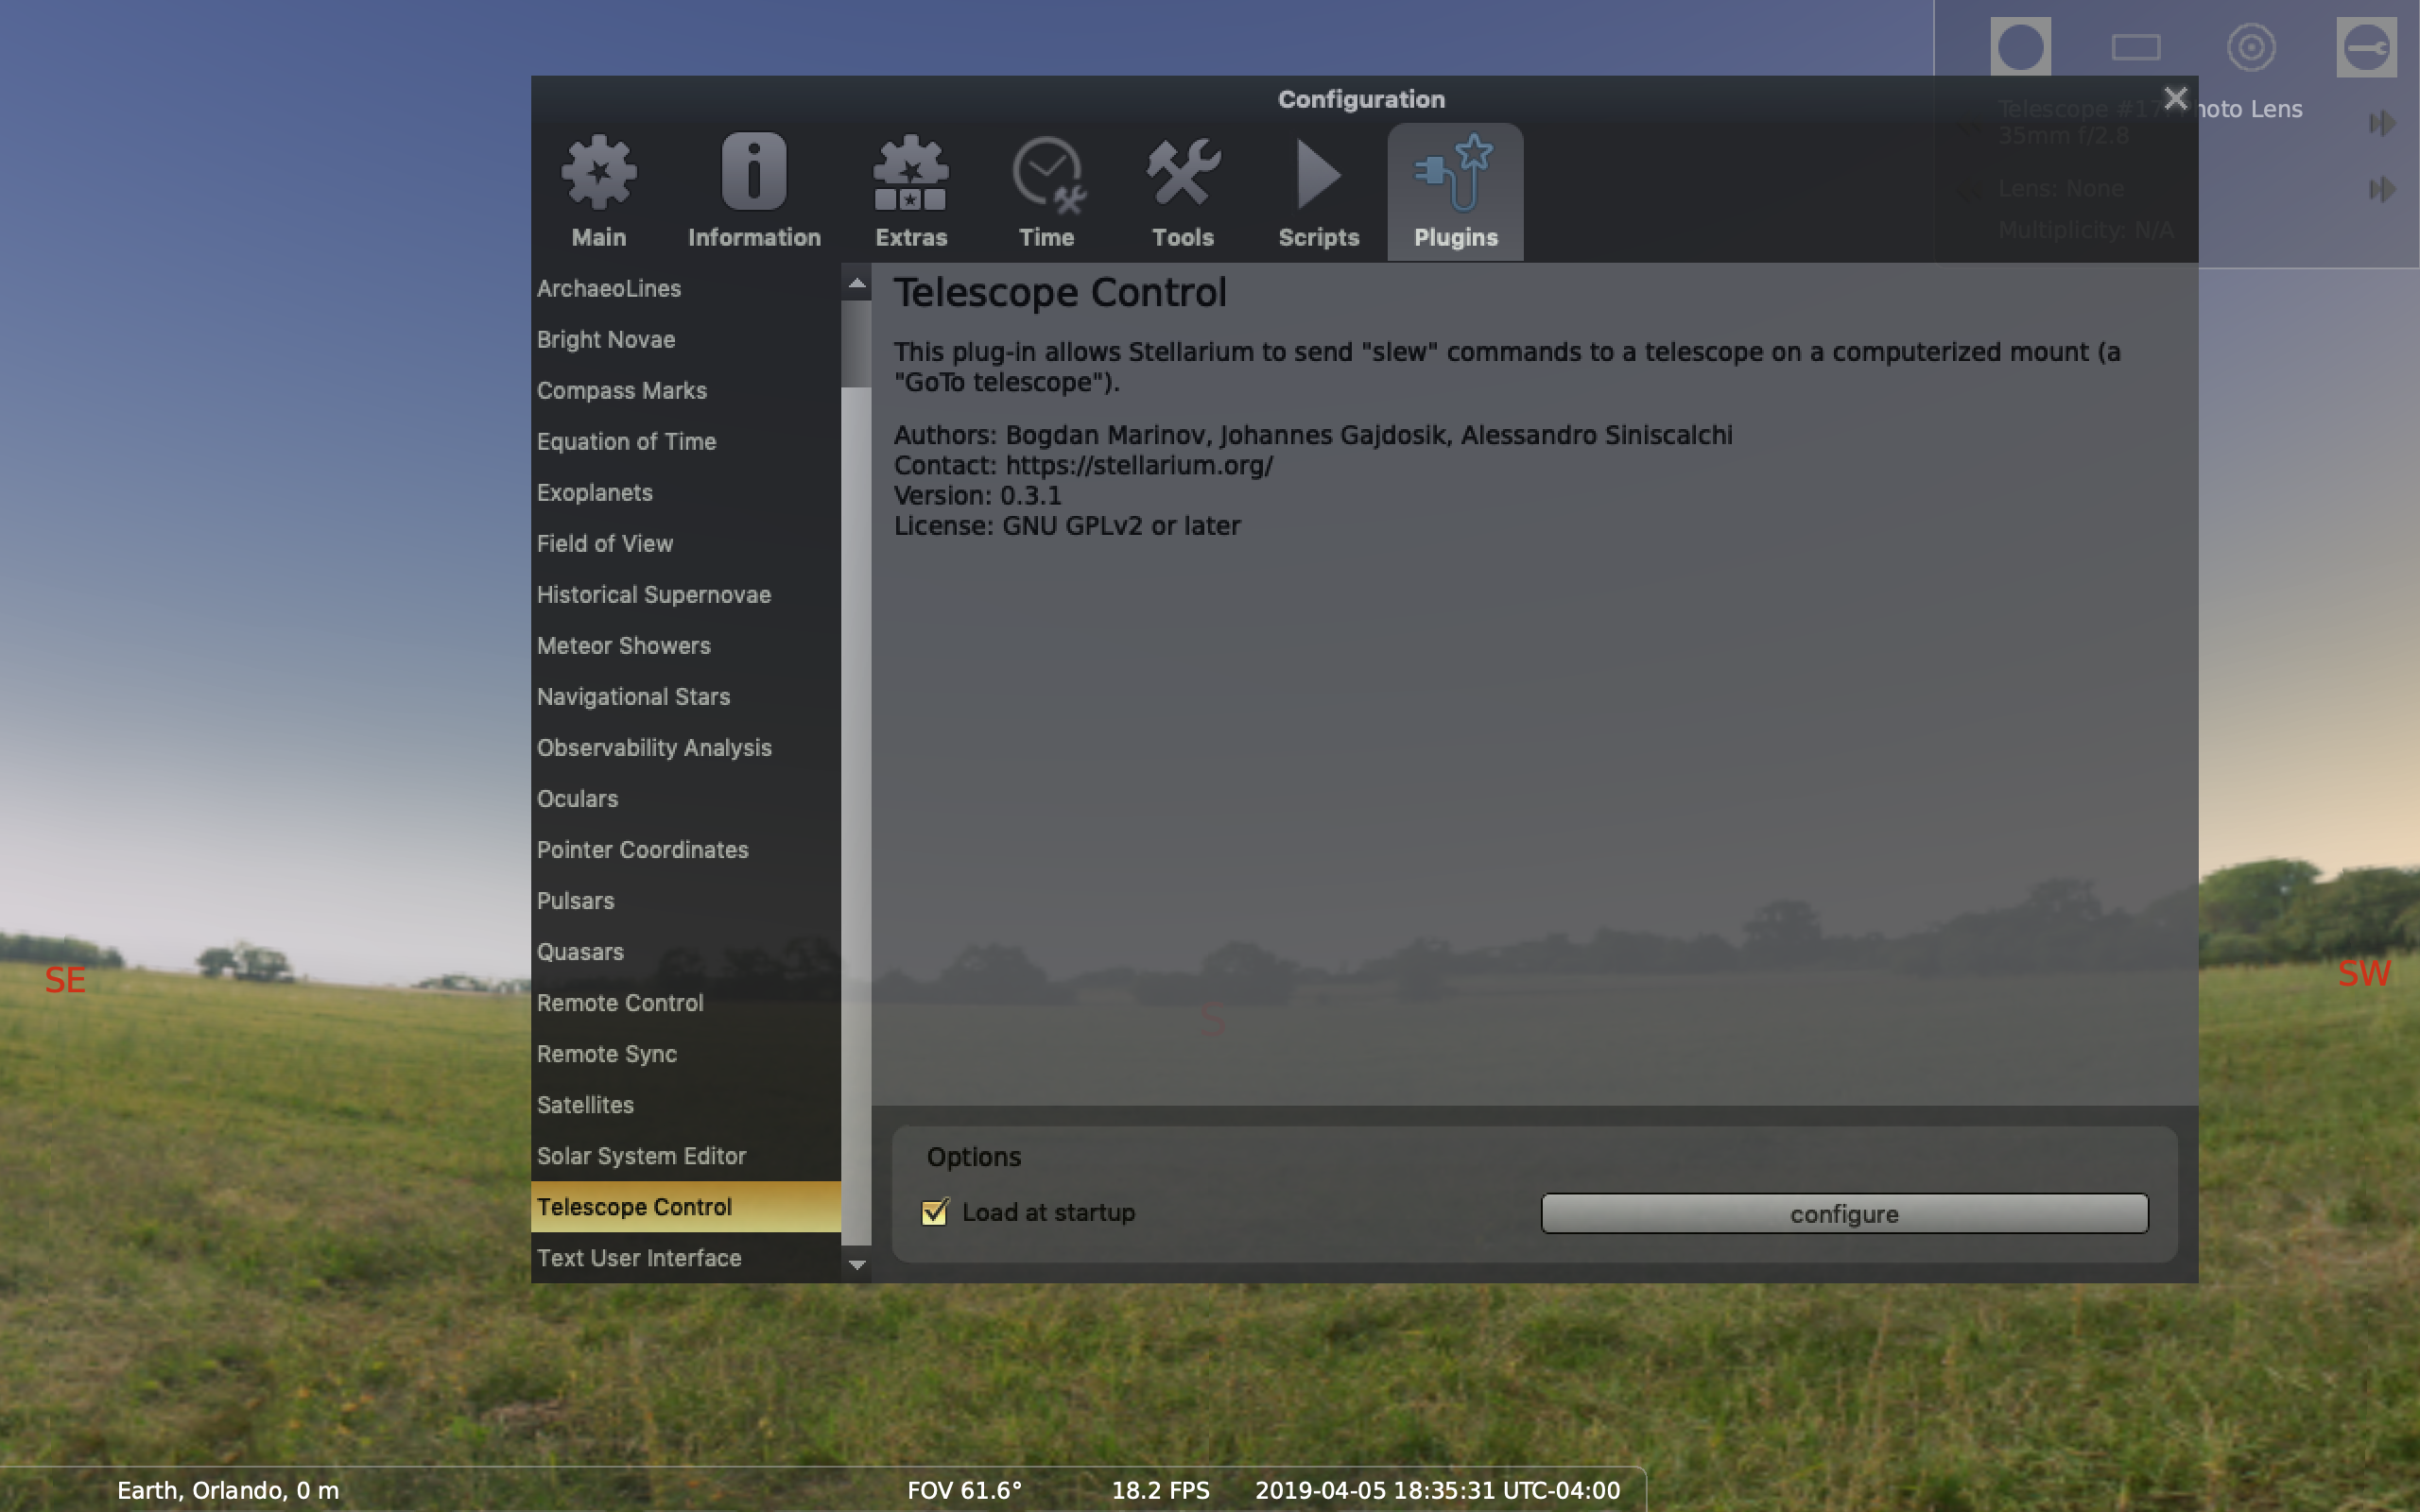
\includegraphics[width=1.0]{stellTeleWindow}
\end{figure}

  5. Ensure “Load at startup” is selected at the bottom on the window and Select “Configure” next to it.
  6. Select Add to create a new telescope.
  7. In the new window (displayed in the image below), select the first option “Stellarium, directly though a serial port”.
  8. Next ensure the coordinate system is set to “Equinox of the date (Jnow)” and the checkbox for “Start/connect at startup” is checked
    -You can also rename your telescope but this is unnecessary
  9. Finally, select Ok at the bottom of the menu. You will be placed back to the telescopes overview page where you can see whether the telescope is connected and the number associated with the telescope.

\begin{figure}[h]
	\centering
	\caption{Stellarium Telescope Configuration}
	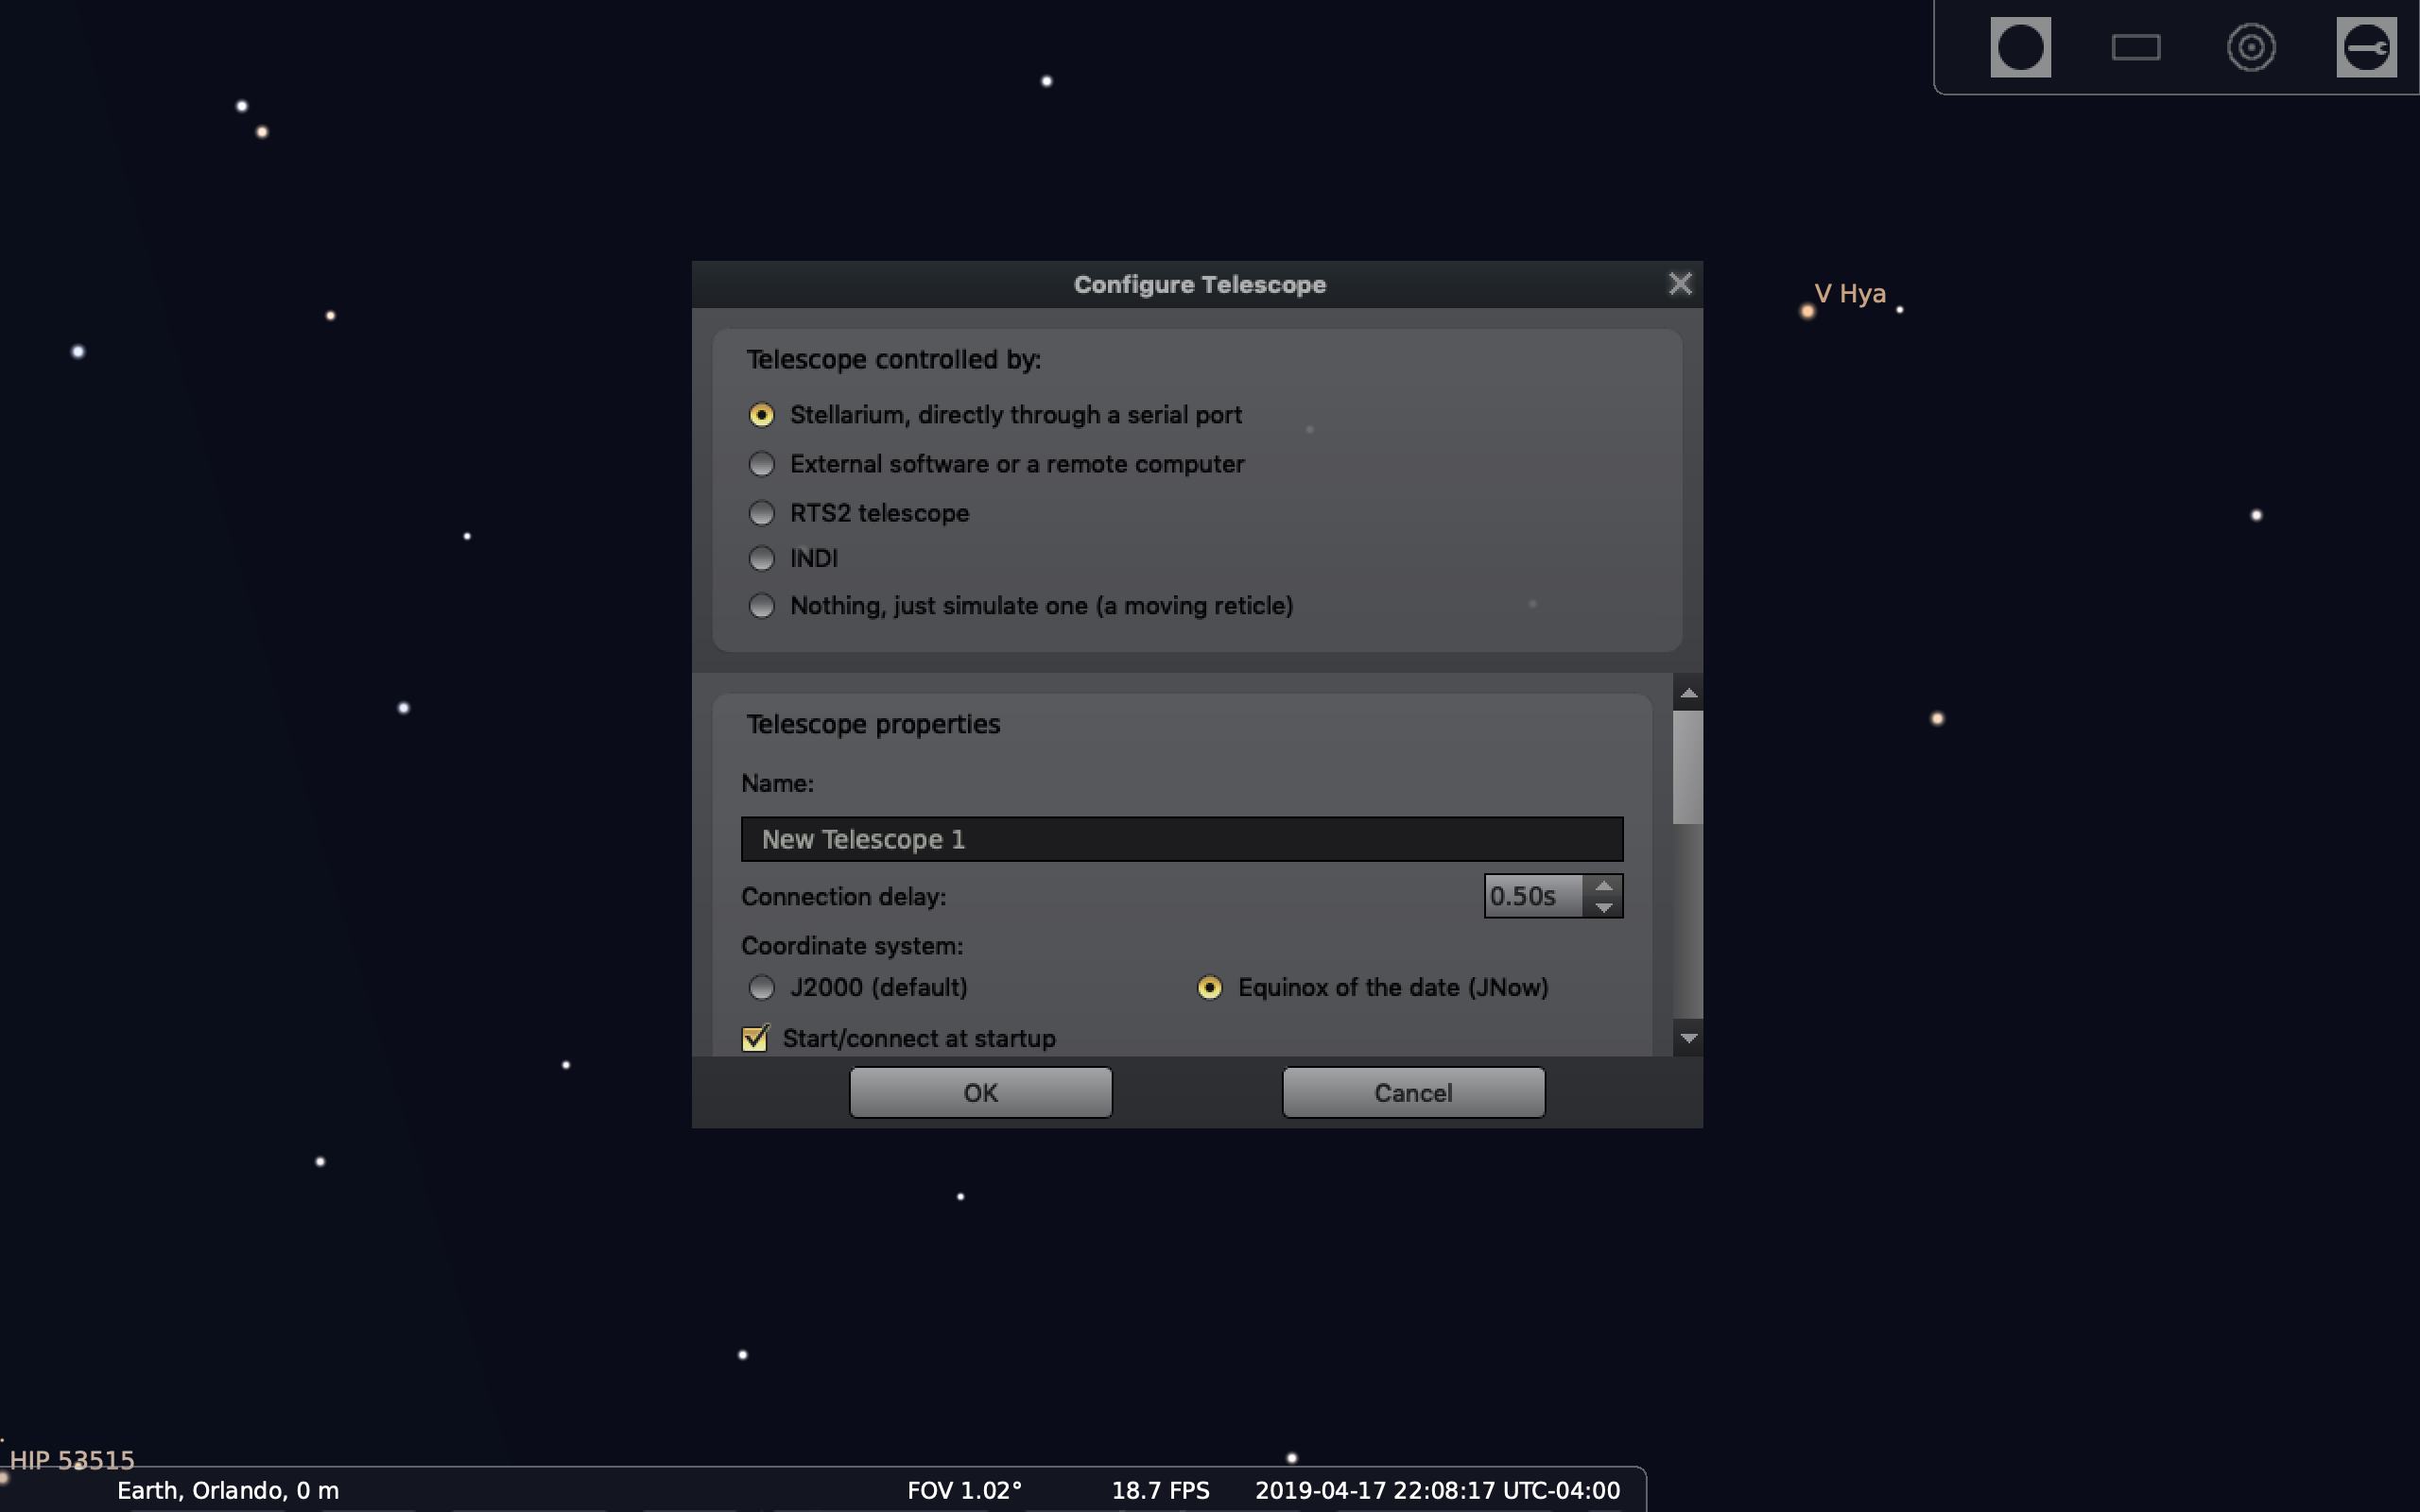
\includegraphics[width=1.0]{stellConfig}
\end{figure}

Each Subsequent Use Setup: Ensure Stellarium recognizes the connection to your telescope by visiting the configurations menu again.

Telescope Control
	1. Select and click the object you wish the telescope to point at and
	2. Press CRTL + (the number associated with the telescope)

Finally, it is important to always ensure Stellarium is in equatorial mode and not azimuth mode. While this toggle does not change the output strings to the telescope, it does help the user view the correct orientation of the sky related to the equatorial mount being used. Objects in the sky are displayed in different locations when switching between modes, which can lead to confusion. This confusion can lead to the thought the telescope may not be pointed in the correct location. This option can be toggled between using CRTL + M or by selecting the option from the menu on the bottom. The toggle can be seen on the bottom menu in the fifth box from the left in the first slot. The button is a telescope with a dotted ‘x’ in the back. It is in equatorial mount mode when the toggle is lit up. You can also have the program display a message indicating the mode everytime you switch. Under default settings this option is not chosen, so the user needs to open the configuration settings window and select tools from the available tabs. In the tools window about halfway down the options, there is a checkbox named “Indication for mount mode” located to the left of “Dithering” option.

\subsection*{Celestial Coordinates}

In Stellarium, the current coordinates provided for right ascension(RA) and declination(DEC) are sent as celestial coordinates, also known as equatorial coordinates. Cartesian coordinates are the standard for most locations like determining the location of the Robinson observatory or Paris, France. These locations are constructed through latitude and longitude and do not rely on time. These coordinates can be easily manipulated with sine, cosine, and tangent to find other pieces of the location. The same is not present with celestial coordinates.

Since the sky is constantly moving, astronomers formulated coordinates to use for this constant change instead of using typical cartesian coordinates. Somewhat relating to normal coordinates, right ascension is similar to longitude while declination is similar to latitude. Declination starts at the celestial equator. The celestial equator extends from the Earth’s equator onto the celestial sphere. This sphere is fictional but helps you understand what parts of the sky you can see. This sphere is not relative to the horizon but rather where you are and informs you anything above the horizon you can see but anything below the horizon can’t be seen. Right ascension relates to the vernal equinox. This is an arbitrary point chosen each year where the Sun appears to cross, since the celestial sphere is fictional, the celestial equator when moving from south to north (reference). Starting at this point, right ascension is 0 degrees and increases eastward while declination is 0 degrees and increases upward. The coordinates are sent by Stellarium in hours, minutes, and seconds for right ascension and degrees, arcminutes, and arcseconds for declination. These two strings are currently sent in the template provided below and are distinguished by the start with either :Sr for right ascension and :Sd for declination.

\begin{figure}[h]
  \centering
  \caption{Coordinates genreated by Stellarium}
  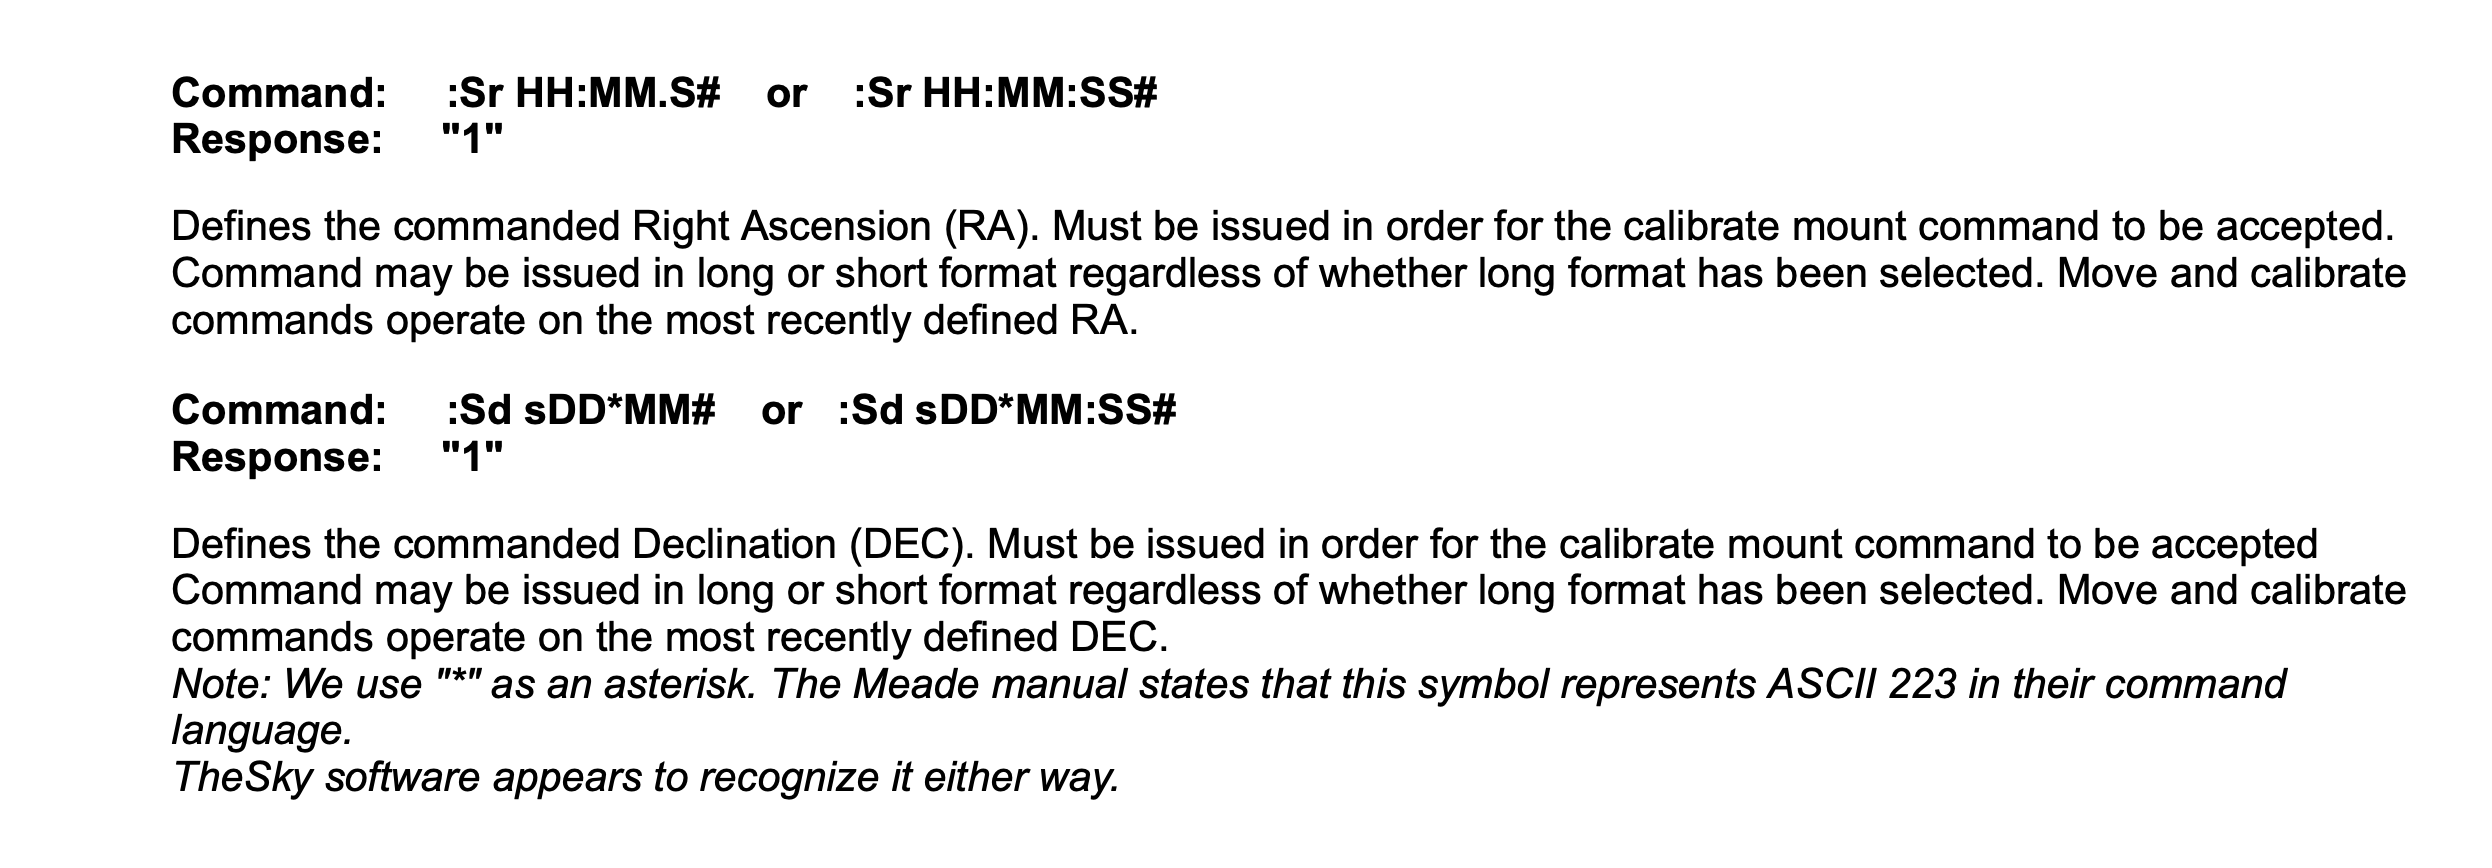
\includegraphics[width=1.0]{convStell}
\end{figure}

The tricky part of celestial coordinates are they are constantly changing because the celestial coordinates are directly impacted by the orientation of the Earth. An orientation that goes through 26,000 year cycles. With this constant change, coordinates are derived from the current epoch or through the equinox of the date. An epoch is reference point used for a moment in time (reference). We are currently in J2000 with the next update coming in 2050. It is important to note Stellarium lets us decide what reference of time we will use for object locations. If the system is ever changed in the settings, the telescope should be immediately recalibrated or the telescope will not point to the correct location. With this dependency with time, a real time clock needs to be in use when coordinates are formulated along with slew commands. This requires all conversions to be handled within Stellarium and not the Arduino board. The board has no room to hold the micro controller needed for a real time clock.

Conversions can be made between celestial and cartesian coordinates. The distance of the object in either light years or parsecs becomes apart of the equation though. These conversions are usually only helpful when dealing with an altazimuth mount. This mount has two motors like the german equatorial mount but deal directly with vertical and horizontal movement relative to the ground below. German equatorial mounts take into consideration the poles of the Earth before the assembly of the right ascension and declination motors. With these differences, converting between celestial and cartesian would provide extra steps when calculating slew commands and thus are unnecessary. We will keep our coordinates in celestial to maintain a standard with the slew command process.

\subsubsection*{Mathematical process for telescope pointing}

First off, it will be important to calibrate the telescope so that the home position relates exactly to the vernal equinox. The vernal equinox for this year, 2019, will happened on March 20 at 5:58 Eastern Standard time. To help calibrate the telescope to this position when the time comes, we will use the current location of the Sun at that time in altitude and azimuth. These coordinates work well here as they are absolute positions in the current sky and don’t rely on time. We would use this position as our base then use the Sun’s celestial coordinates to move to the vernal equinox. This is done by moving to 0 degrees RA and 0 degrees DEC. This step will only need to happen upon first use of the telescope. After that, the home position will be saved to memory.

To provide the slew instructions for an object selected, we need to receive the current degree placements of both motors from the Arduino board. These readings sent from the Arduino board will tell the change from the standard home position of the telescope instead of the telescope’s actual location. So first, we will need to take the readings from home position and compare them to the standard home position. This will give us the current viewing location of the telescope. Then from that position, we can take the difference between the telescope position and the current object to be tracked position to provide the correct instructions. This requires us to convert the Stellarium strings for RA and DEC to degrees. The math is provided in the image below. Declination is pretty straight forward in conversion to degrees but right ascension requires the conversion to degrees than the multiplication by 15. This accounts for the fact the Earth moves about 360 degrees in 24 hours resulting in 15 degrees an hour. Furthermore for both conversions, minutes for RA and arcminutes for DEC are divided by 60 to account for 60 minutes in an hour. Next seconds  for RA and arcseconds for DEC are divided by 3600 to account for 60 seconds of 60 minutes in an hour. One last step for declination is applying the sign of the original coordinates given by Stellarium to the newly converted degrees. This only happens for declination because right ascension is always positive. Right ascension only ever calculates eastward. Declination can calculate both upwards and downwards relative to the celestial sphere.

\begin{figure}[h]
  \centering
  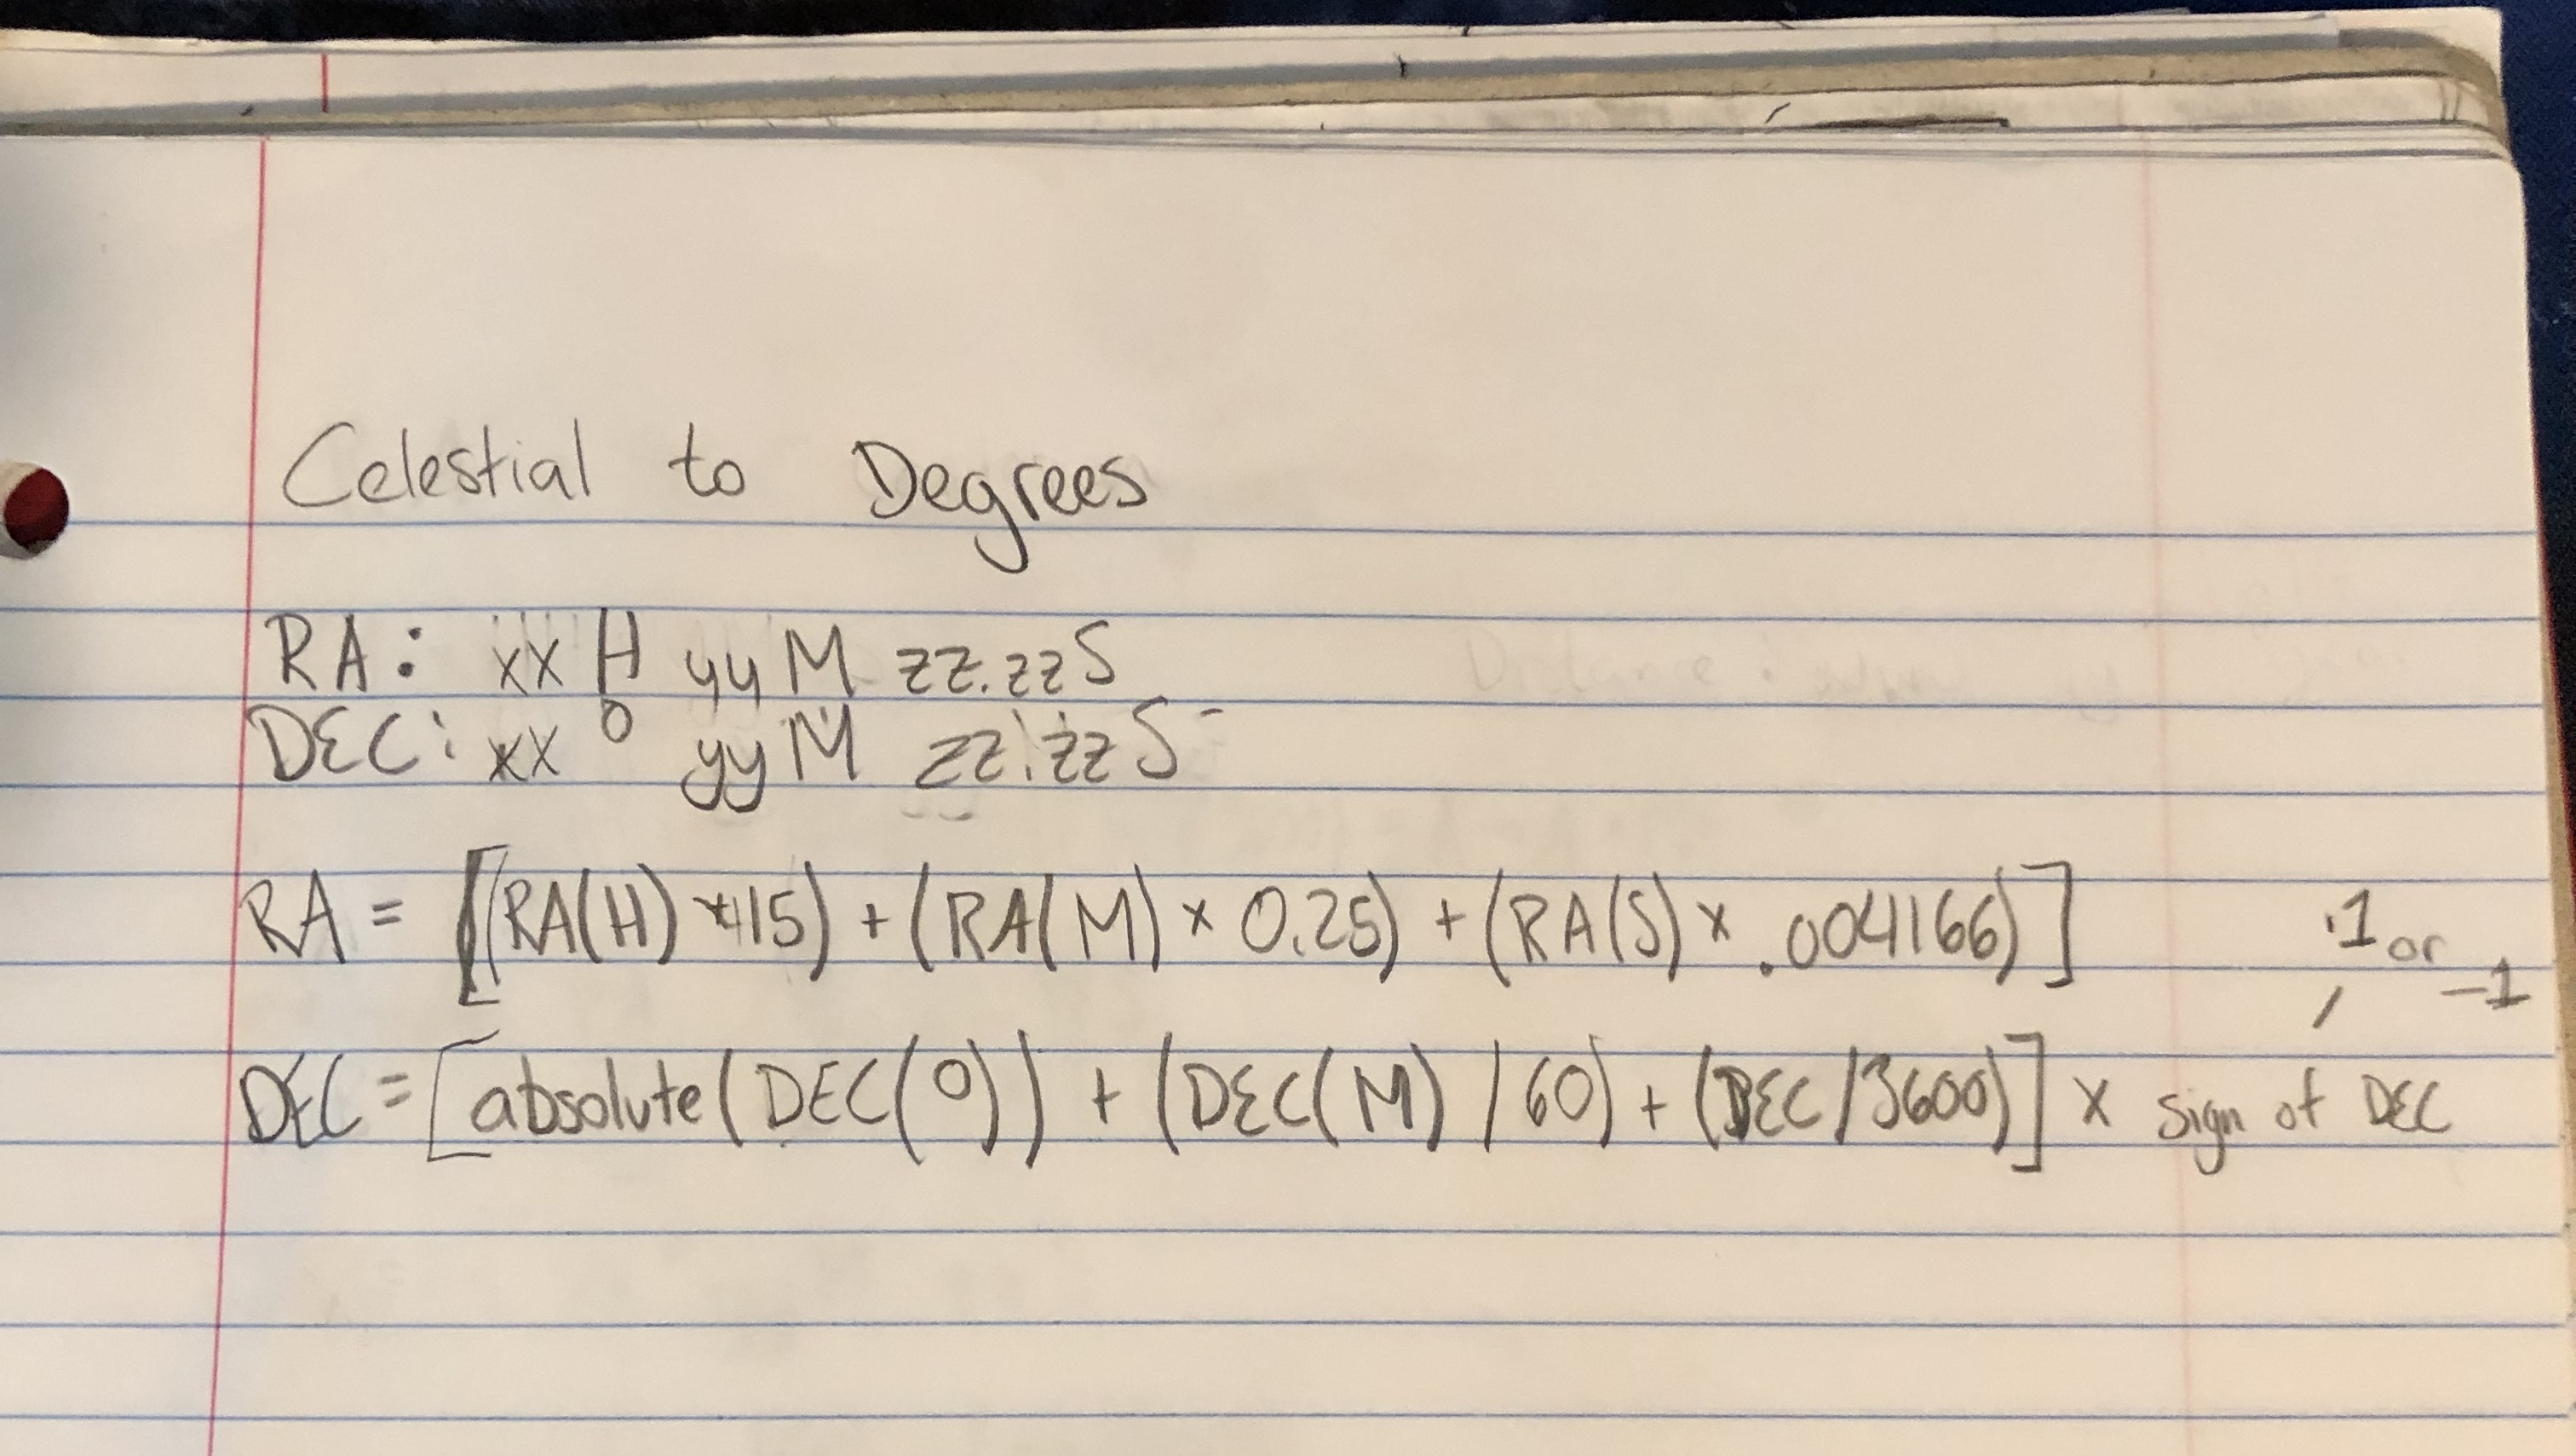
\includegraphics[width=1.0]{convMath}
\end{figure}
\begin{figure}[h]
  \centering
  \caption{First image shows formulas, Second image provides example of process}
  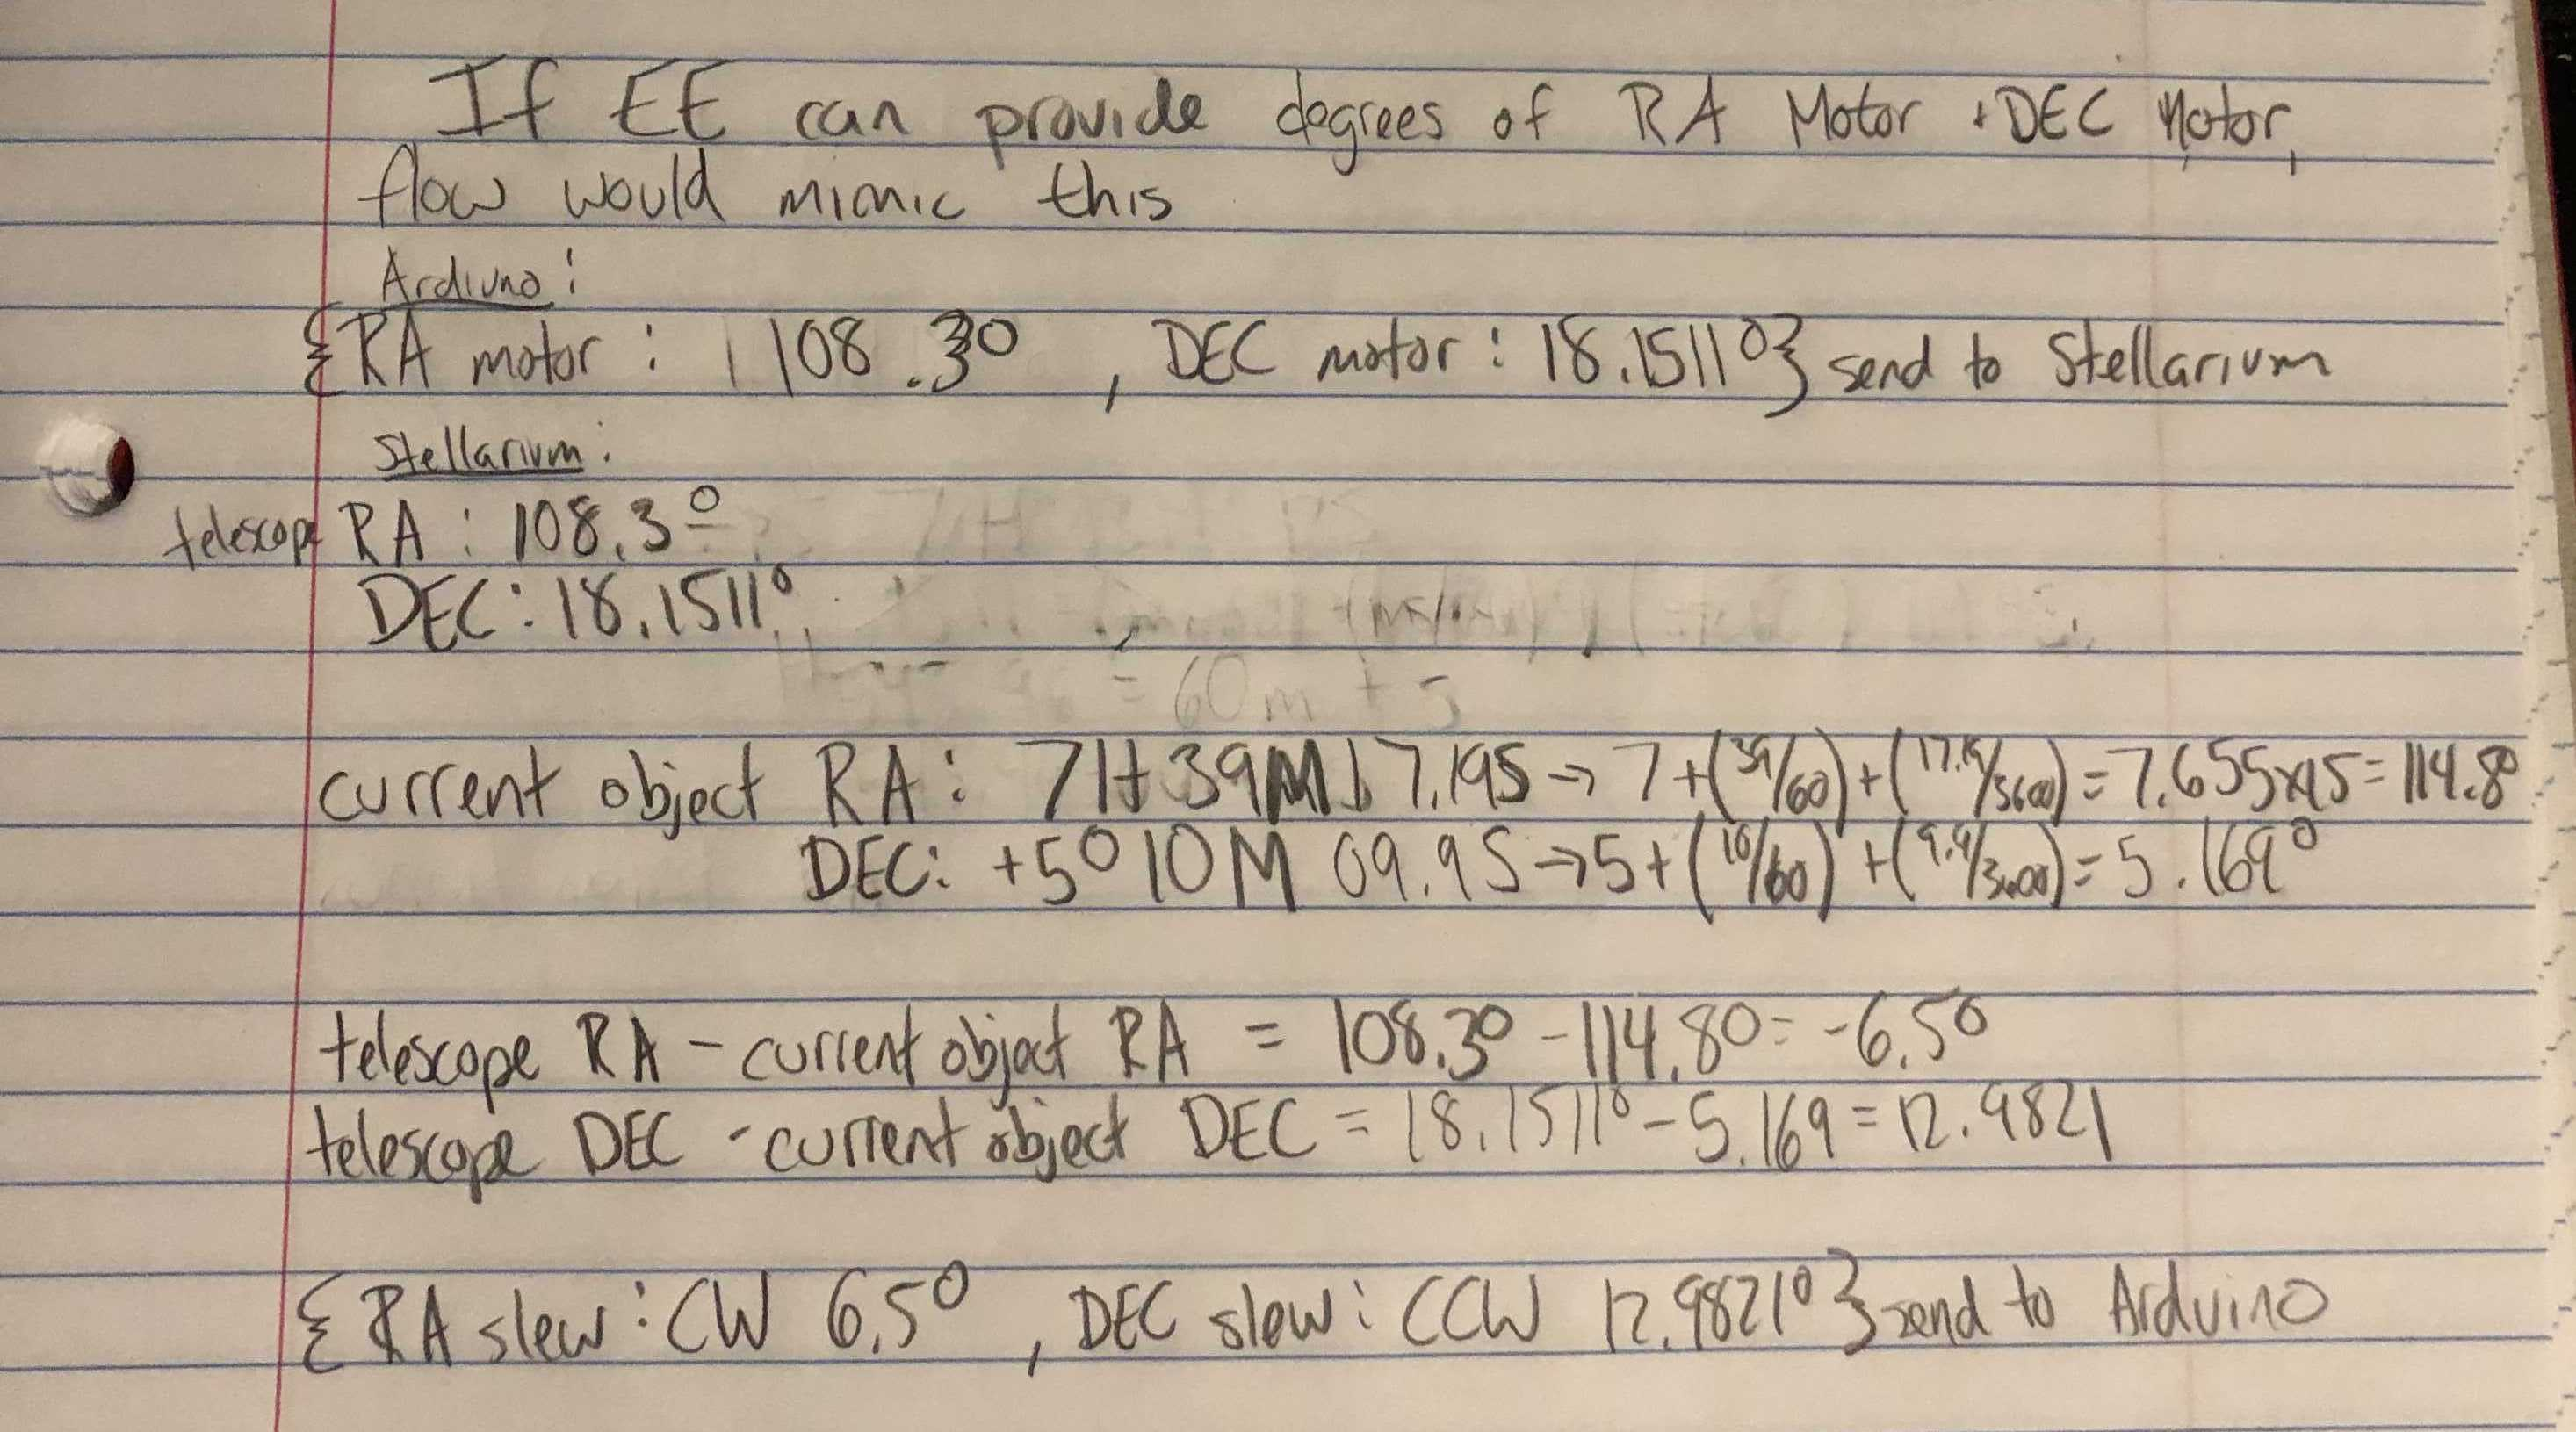
\includegraphics[width=1.0]{convExample}
\end{figure}

\subsubsection*{Meridian Flip}

Coordinate conversions is not the only math we need to add to Stellarium. We also need to formulate a meridian flip. A meridian flip can be implemented in a few ways on a telescope like through a physical switch or through software implementation. We will focus on the software implementation where before we send a slew string to the Arduino we will have already accounted for the meridian flip if needed to complete the slew.

This flip is only needed on equatorial mounts because the telescope is aligned with the polar axis. The meridian is another circle in the celestial sphere that passes through the zenith, nadir and the two celestial poles. The zenith is directly above where a person is located. This point is marked on the celestial sphere. Conversely, the nadir is directly beneath where a person is located. This point in marked on the opposite end of the sphere. Once these points are found, the meridian can be determined.

When the telescope passes this circle in the celestial sphere, a reorientation needs to be performed. Without this reorientation of the telescope, it may lead to the damage of the mount or motors if the telescope is pinned against itself but keeps trying to move. So this flip needs to be implemented in two ways. The first is when tracking an object from the West side of the meridian to the East side. The second is when tracking an object from the East side of the meridian to the West side.

A meridian flip is unique to each telescope as the dimensions of telescopes are different so there is not a standard where your telescope will collide with itself at a certain position past the meridian. This limit will need to be researched once our telescope is built. If a slew will cause the telescope to travel past the limit we define, we will reorientate the telescope so further tracking of the object is possible.

\begin{figure}[h]
  \centering
  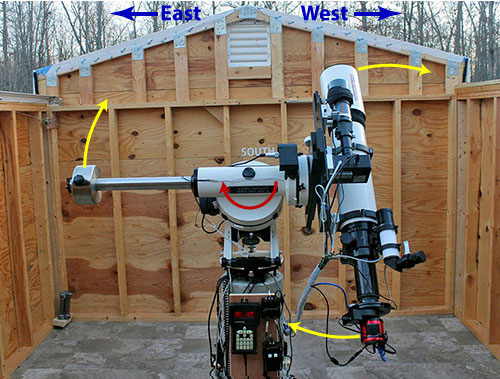
\includegraphics[width=1.0]{beforeflip}
\end{figure}
\begin{figure}[h]
  \centering
  \caption{First image on left is start of tracking. Second image on right shows tracking after flip.}
  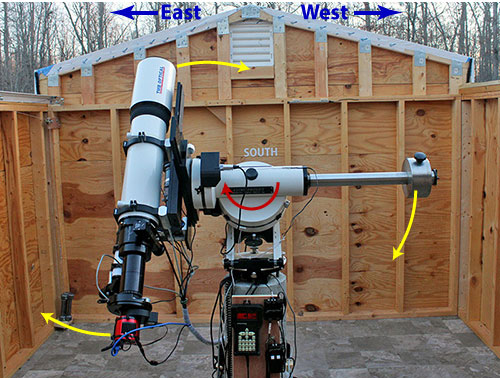
\includegraphics[width=1.0]{afterflip}
\end{figure}

To help give a visual idea of the meridian flip, three images are supplied below. The object being tracked started to the east of the meridian and moves westward while remaining at a DEC of 0 degrees. As the telescope tracks westward, the first image shows the end of the telescope would hit the mount if the telescope stayed on its current course. To avoid this, we would send to the Arduino to start rotating the RA motor counterclockwise from its current location while the DEC motor rotates 180 degrees clockwise. This flip is shown in image two. The telescope will not end up pointing to a new location. Rather the mix of these movements will result in flip over the ‘y’ axis of the mount as shown in the third image. The DEC motor will once again be pointed to 0 degrees while the RA motor will be pointed to the same degree it had before the flip but can now keep tracking westward.

\begin{figure}[h]
  \centering
  \caption{Telescope while performing meridian flip.}
  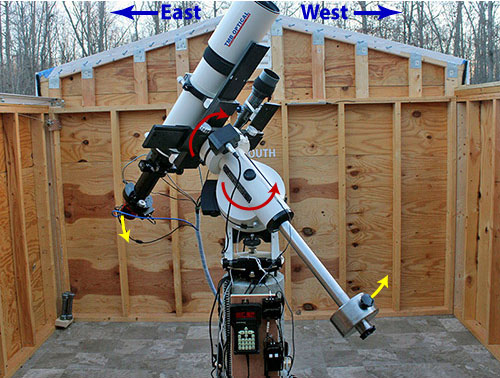
\includegraphics[width=1.0]{duringflip}
\end{figure}

What does this mean for our communications between Stellarium and the Arduino? If the flip happens during the tracking of an object, tracking must halt and the end coordinates need to be saved while the flip occurs. We will take control of the telescope while the flip happens thus the coordinates need to be saved so we can reinitialize the slew after the flip has been processed. This will be implemented so our flip commands and slew commands do not tamper with each other. The strings outputted by the meridian flip will not be telling the telescope about a new point in the sky and thus will be the same no matter where the flip occurs. The DEC motor will rotate 180 degrees and then the RA motor will rotate counterclockwise until the original DEC location is achieved. Next, Stellarium will need to take in a new command outside the LX200 protocol for a manual annual meridian flip initialized by a button on the telescope. This command will call the same meridian flip function as used during object tracking but our software would not have known the need to do so without the command from the Arduino.



\section*{Archive Frontend}

The data gathered by the telescope will need to be accessible by future researchers. Likewise, it might be possible to allow the general public to have access to the data. Either way, the data archive will require a frontend to enable browsing, searching, uploading, downloading, and categorizing the data. The frontend will be a login secured website in order to maximize portability and accessibility. By foregoing a native application, we ensure that the data will be accessible from anywhere with an internet connection. Likewise, we enable the researchers to utilize whatever person computers are most convenient. i.e. laptops, a tablet, an iPad, a cell phone, etc.

Figure \ref{fig:archiveusecase} shows a high level overview of the archive frontend. Each action of the archive system performs modifications in the database when they are accessed by the end-user. The actions will be accessible via the interactive website or via the API directly. This separation of function will enable us to potentially expand our project scope as needed. There may be other applications that can utilize the API as part of our project or future projects.

\begin{figure}[h]
	\centering
	\caption{Archive Frontend Use-Case}
	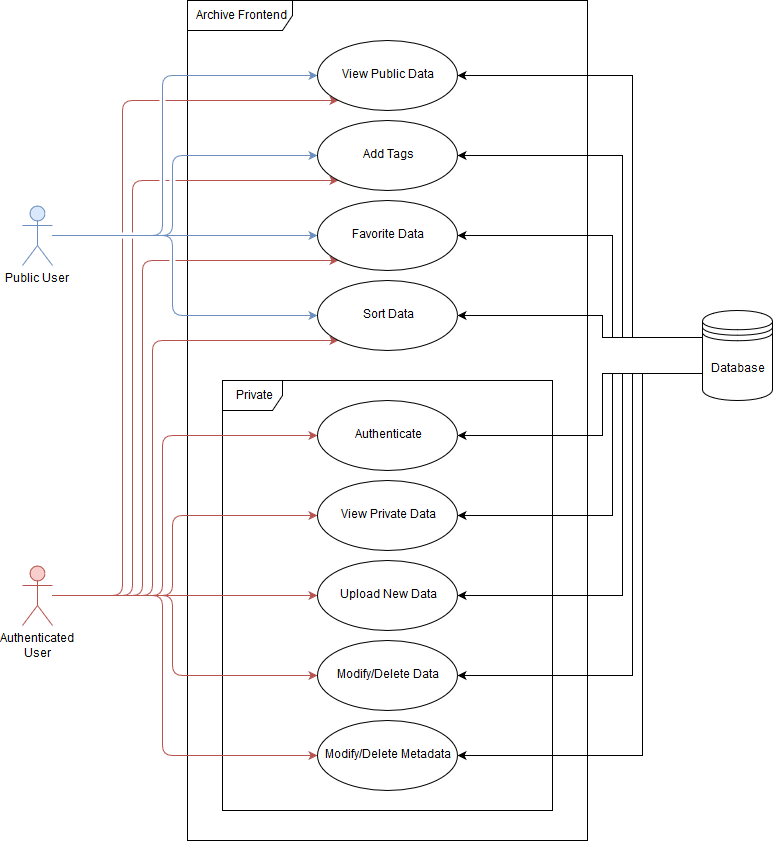
\includegraphics[width=0.75\linewidth]{frontend_use_case}
	\label{fig:archiveusecase}
\end{figure}

The archive will be split into two separate components. Access to the private portion of the website functionality will require logging-in so that the user can be authenticated. Likewise, different users may have access to different sources of private data depending on the security needs of the observatory.

Unauthenticated users will be able to browse the data published as public. We enable said users to perform basic browsing and searching as one would expect. Likewise, we will enable users to add tags and favorites to data. Said information will be stored in the user's cookies until they decide to create an account. Once an account is created, the data stored in their cookies can be uploaded to ensure that the data is persistent across browser sessions.

Authenticated users with the appropriate account permissions will have access to further functionality beyond the basics. They will be able to modify the database directly by uploaded new data and modifying the metadata associated with data that exists withing the archive. Any modifications made by an authenticated user will only apply to data within their permission group. Data may be shared across several permission groups and thus users will only see the modifications made associated with their group. In order to facilitate said functionality, we will need to keep modifications separate from the source data in our backend.

\subsection*{Frontend Frameworks}

Frontend frameworks have become the de facto standard of the web. Industry has moved away from static HTML websites in recent years. Users demand a high degree of interactivity from their websites. Thus, industry has responded by adding more client code in order to facilitate said demand. By utilizing a framework for our project, we will gain vital industry experience that employers are looking for from their applicants.

We opted to utilize a frontend framework in order to facilitate a high degree of interactivity. There are several options for delivering static HTML pages with minimal client-side JavaScript. However, we want to ensure that our client interactions are extremely fast to load. Specifically, sorting data can be offloaded to the client to ensure that one doesn't have to load a new web-page each time that one changes a search parameter. Utilizing a frontend framework enables us to update the data display instantly when said parameters are changed.

There are many modern frontend frameworks which enable developers to quickly create highly interactive websites efficiently. Our frontend solution will need to be data efficient to reduce the strain on potentially poor connections. It is possible that potential users will have a poor internet connection while attempting to access the data. (As is the case in some observatories.) Thus it is necessary to choose the appropriate framework solution which enables rapid development while maintaining a focus on efficiency.

\begin{figure}[h]
	\centering
	
\includegraphics[width=0.251\linewidth]{angular}
\end{figure}

\subsubsection*{Angular}

The Angular web framework was released by Google in September of 2016.\cite{angularrelease} Angular (also known as Angular 2) was released as a replacement for Angular 1. Its release focused on "a wide range of use cases,...[optimization] for developer productivity, small payload size, and performance."\cite{angularrelease} The framework was built from the beginning via "collaboration with the open source development community."\cite{angularrelease} Thus it has received input from many different developers to ensure that it is flexible enough for general use.

Angular utilizes TypeScript as its implementation language which helps reduce bugs associated with loose typing. Typescript also brings many features absent from plain JavaScript which can help to reduce developer time. Utilizing a framework which already utilizes TypeScript will be more advantageous than trying to use it with a framework which was not built to support it.

Angular is built utilizing component objects. The Angular official quick start guide states that "components are the fundamental building blocks of Angular applications."\cite{angularquickstart} These components "display data on the screen, listen for user input, and take action based on that input."\cite{angularquickstart} Components are a good way of breaking one's code up into reusable pieces. By compartmentalizing one's code in this way, there is a reduction in the duplication of effort. Likewise, it creates the opportunity to test each component separately from the rest of the overall application.

Angular is a good candidate for our archive frontend. It was designed to be extremely flexible. Likewise, it is a commonly used industry frontend framework. Employers look for candidates with existing knowledge of frameworks. Thus it would be useful for our team to gain experience using such a common library.

\begin{figure}[h]
	\centering
	
\includegraphics[width=0.25\linewidth]{bootstrap}
\end{figure}

\subsubsection*{Bootstrap}

Bootstrap is an open-source framework originally developed at Twitter in 2010.\cite{bootstrapabout} It was originally a closed-source tool for internal use at Twitter. However, it was eventually open-sourced due to its popularity with the internal Twitter developers. Twitter found that "developers of all skill levels [could jump] in without any external guidance."\cite{bootstrapabout}

Like Angular, Bootstrap also includes components. However, the Bootstrap components are focused on the display of data and abstains from opinions about the structure of one's data. This decoupled nature means that utilizing components ensures that applications built with Bootstrap share a common look and feel. Familiar components ensure that potential users are quick to acclimate.

Unlike other frameworks, Bootstrap relies on jQuery to handle its JavaScript integration.\cite{bootstrapjs} Thus, Bootstrap is much less opinionated on the frontend code structure. This enables developers to create their own code idioms and integrate into existing code bases easily. Likewise, Bootstrap is able to be utilized alongside other frontend frameworks. If we chose to do so, we could utilize a framework like Angular and still use Bootstrap to ensure that our look and feel are familiar and consistent for the end users.

Bootstrap's flexibility is both a strength and a weakness. Experienced JavaScript developers will find said flexibility very useful and will be able to structure their code in a familiar fashion. However, our team lacks experience building frontend web applications. Thus, an opinionated framework may become an initial disadvantage. Other frameworks provide a standard way of structuring code and therefore might be more friendly for our team to work with.

\begin{figure}[h]
	\centering
	
\includegraphics[width=0.25\linewidth]{ember}
\end{figure}

\subsubsection*{Ember}

Ember was a JavaScript frontend library released to compete with Backbone.js, SproutCore, Cappuccino, and Dojo.\cite{emberrelease} Many Ember's original competitors have fallen out of the public eye since its release in August of 2012, yet Ember still sees wide adoption even today. Ember was a departure from aforementioned "microlibrary" competitors that were popular at the time of its launch. Ember was different because it focused on "helping developers grapple with the complexity of building 100\% JavaScript web applications."\cite{emberrelease} They did so by "[embracing] the tools that [web developers] were most comfortable with: HTML and CSS."\cite{emberrelease} Thus, Ember was created as an opinionated JavaScript framework which "[helps] you architect large, multi-page applications, but [helps] you to do so without breaking the basic building blocks of the web."\cite{emberrelease}

When a user visits an individual URL in an Ember application the response is handled via an Ember "route".\cite{emberrouting} Routes are how a developer compartmentalizes pieces of their application functionality into reusable components. Thus, it is important to separate one's application based on functionality to ensure that effort is not duplicated among several different routes. Like the other aforementioned frameworks, Ember enables the developer to test individual components by splitting them up into routes.

Ember decouples data from the display routes via objects called "models".\cite{embermodel} Models are a way to adapt the Ember routes to the application's individual data concerns. Thus, Ember provides strong opinions about how one should structure the application's data.

Ember's focus on preserving web browser functionality is definitely an advantage when compared to some frameworks that may cause something as simple as the back button to function incorrectly. Likewise, its opinionated framework style ensures that our team will have a good idea of how to structure our application. However, Ember's rigid structure might be too strict for our purposes. Our team has compartmentalized the web application into frontend and backend sub-teams. Thus, the frontend team needs to be flexible enough to accommodate however the backend structures their data before the frontend interacts with it.

\begin{figure}[h]
	\centering
	
\includegraphics[width=0.25\linewidth]{react}
\end{figure}

\subsubsection*{React}

React was a Framework developed by Jordan Walke at Facebook. It was originally a propriety framework that they used internally. However, it was later released as an open-source framework at JSConf US.\cite{reactlaunch} It was released in 2013 and thus it is a relatively new framework in the JavaScript ecosystem.\cite{reactlaunch} However, it has seen high adoption rates among developers.

React is a single-page web application framework. It enables the developer to dynamically update the contents of a page as data changes or uses interact. Since the web browser doesn't have to load completely new pages with each action, the resultant web application is very responsive since it only downloads information as it is needed without the need to potentially re-download components repeated on each page.

Components are React's way of splitting your application into reusable pieces. Likewise, Components determine how one structures the data on the user's end. React components "[take] in parameters...and [they return] a hierarchy of views to display."\cite{reacttutorial} The data is tightly coupled to the visual model. React's opinionated nature is ideal for our inexperienced developers. A framework like React that provides not only the tools for creating the UI we need but also provides structural guidance is an advantage over the other options available.

React's structure and idioms are a good contender for implementation in our project. The single-page nature of React makes it ideal for places with low-bandwidth connections such as observatories. Likewise, the tight coupling of data and view provides a good starting point for structuring our code. Finally, React is widely used in the industry and so it would be an advantage for our team to gain experience using it.

\newpage

\begin{figure}[h]
	\centering
	
\includegraphics[width=0.25\linewidth]{vue}
\end{figure}

\subsubsection*{Vue}

Vue was released by Evan You in 2014 as an open-source JavaScript frontend framework.\cite{vuelaunch} It received immediate attention from various web communities and it has developed significantly since its launch. It is being actively developed and receives regular bug-fixes and stability patches. Despite its relative immaturity, the framework has seen wide adoption due to its progressive design philosophy.

Vue is compartmentalized across several different libraries. The core library "is focused on the view layer only, and is easy to pick up and integrate with other libraries or existing projects." \cite{vueguide} However, Vue optionally has the capability to "[power] sophisticated Single-Page Applications when used in combination with modern tooling and supporting libraries."\cite{vueguide} Vue's flexibility enables it to integrate into many differing use-cases.

Like the other libraries examined, Vue also supports component composition via Vue's component system. This abstraction system is "an abstraction that allows us to build large-scale applications composed of small, self-contained, and often reusable components."\cite{vueguide} They can be nested and pass data from parent to child. Data passing is done via props and a specialized binding syntax.

Utilizing Vue for our project would mean depending on a relatively immature library. However, its lightweight molecularity will enable us to only utilize the components that we need for our project. By doing so, we will reduce both the complexity of our resultant application and the bandwidth requirements associated with loading the libraries. Likewise, the single-page application nature of Vue will also reduce the amount of data being utilized.

\subsection*{Frontend Programming Languages}

JavaScript is a ubiquitous frontend programming language for use in the browser. Recently, it has also gained popularity in the native application domain via Node.js. Node.js is a open-source cross-platform run-time environment which enables existing JavaScript developers to leverage their skills on the backend. However, despite JavaScript's popularity there are several alternatives that seek to eliminate some of JavaScript's intrinsic pitfalls.

\begin{figure}[h]
	\centering
	
\includegraphics[width=0.25\linewidth]{coffeescript}
\end{figure}

\subsubsection*{CoffeeScript}

CoffeeScript is a language that compiles down to JavaScript.\cite{coffeescriptlittlebook} However, "CoffeeScript is not a superset of JavaScript, so although you can use external JavaScript libraries from inside CoffeeScript, you'll get syntax errors if you compile JavaScript as is."\cite{coffeescriptlittlebook} This sacrifice of direct compatibility comes with sever advantages. Notably, CoffeeScript's succinctness means that the developer typically has less code that they directly have to write.

CoffeeScript has many interesting syntactic features that enable developers to express code concepts more succinctly than plain JavaScript. One such feature is comprehensions.\cite{coffeescriptguide} Comprehensions can replace loops in a more readable fashion and read a lot like English sentences instead of code. Comprehensions greatly shorten the amount of code required to express an idea. Many problems that can be solved via comprehensions are common and may occur across many use cases. The overall style of CoffeeScript borrows from languages like Python, Ruby, and Haskell. Thus, it is very readable and has a focus on clean code paradigms. This readability means that code concepts are parsed more quickly by developers and reduces the chance of confusion when reading source code.

CoffeeScript, once transpiled, runs as plain JavaScript in the client's browser.\cite{coffeescriptguide} This transipation process means that CoffeeScript is compatible across the many different browsers that already support JavaScript by default. However, CoffeeScript utilizes modern JavaScript features.\cite{coffeescriptguide} Thus, it might not be able to run on older browsers which lack support for modern JavaScript. The trad-offs between developer features and client compatibility is some that one must consider whenever choosing a language/library for use. However, our rapid development time-frame might benefit from languages that reduce the amount of necessary boilerplate.

The other languages explored are statically typed; CoffeeScript is not. Dynamic typing can be a double edged blade. It enables rapid development which would be a boon for our team. Likewise, since the code is dynamically typed, it is very flexible. This flexibility ensures that code is resilient to changes in the code base that might require massive refactoring otherwise. However, dynamic typing also has a sinister side. Many bugs which are essentially impossible in a statically typed language can manifest in a dynamically typed language like CoffeeScript. Likewise, it is much harder to develop tools for a dynamically typed language. Type inference can bridge the gap somewhat but it does not yield the same fidelity of information that statically typed languages confers. Thus, the resultant tools associated with a dynamically typed language like CoffeeScript are somewhat weakened by the lack of strong types. Tools are a vital part of developing modern software and our team needs all the help we can get. Thus, the lack of extensive CoffeeScript tools are a potential downside that must be considered before our team commits to utilizing it for as our frontend language.

Like some of the less popular frontends, utilizing CoffeeScript in our project would mean taking a gamble on a product that isn't as widely used as other solutions. Maintainers that come after us would need to be able to service the code without being tripped up by a potentially defunct programming language. However, there is an upside. CoffeeScript's features and syntax would mean less lines of code for our team to write. Language expressiveness is an often overlooked feature when planning a project. Utilizing the right tool for the job is an essential part of the planning process.

\begin{figure}[h]
	\centering
	
\includegraphics[width=0.25\linewidth]{dart}
\end{figure}

\subsubsection*{Dart}

Dart is a general purpose programming language developed by Google as an open-source alternative to existing solutions.\cite{dartlaunch} It was designed to be "structured yet flexible" and to "deliver high performance on all modern web browsers and environments ranging from small handheld devices to server-side execution."\cite{dartlaunch} It was launched by Google in 2011 and has seen varied adoption across different use-cases.

Like the other options explored, Dart can also be transpiled to JavaScript for execution in modern web browsers. It even benefits from compile time optimizations that can, "in some cases, run faster than equivalent code hand-written using JavaScript idioms."\cite{darttalk} The compilation process eliminates the need for some checks and operations that would otherwise need to be performed at run-time. Thus, the resultant code is very fast indeed.

Dart also features prominence in the mobile application space. Google has developed their Android/iOS alternative Flutter for use with the Dart programming language.\cite{darthomepage} Dart runs naively on x86 and ARM computers. Likewise, it also supports a run-time environment with a built in garbage collector and a mature set of core libraries to ensure rapid, safe development of mobile applications. Utilizing Dart for our frontend code would mean gaining a unique skill-set applicable to a blooming mobile application space.

Dart is statically typed with a focus on object-oriented design paradigms. Its syntax was strongly influenced by existing programming languages such as C, Java, C\#, and JavaScript. Thus, it is a highly approachable language that should feel familiar to most developers. This ease of adoption is important for the rapid acclimation of developers on a project. Likewise, it would behoove our team to use a language that is easy to pick up and use due to our limited development time.

Like the other languages explored, Dart has a unique set of tools associated with the language. One such feature is the code analyzer. Its use before deployment can catch bugs before they become an issue in production code. For instance, said analyzer will be able to detect if you fail to cover all possible cases when utilizing enumerations in a switch statement. This small reminder seems trivial at face value but it can cause a lot of headaches if the developer doesn't anticipate it in advance. Likewise, it enables the developer to add new enumeration values without fear. This can be done because once one adds the new values, the analyzer will alert the developer to all the switch statements that need to be modified to include the new enumeration values. Tools like the Dart analyzer are a strong motivation to choose a language alternative to plain JavaScript. Given our teams relative inexperience, we would greatly benefit from such tools and our resultant code will be better as a result.

Utilizing Dart in our frontend would also mean relying on yet another library. Dart has strong opinions about code structure and static typing. Thus, we would need to utilize a middleware library to act as a bridge between our Dart code and whatever frontend library we choose to utilize for implementation. It is possible that any of the libraries that we choose to implement our project may become unmaintained and fall into disuse. Reliance on yet another library reduces the maintainability of our project if future senior design students are tasked with updating, maintaining, or expanding our code. Such an eventuality must be considered before we include yet another library in our project.

Dart represents the unique opportunity to be at the forefront of Google's vision of future application development. It is possible that the mobile market will shift towards a uniform platform like dart in the future. Our team would benefit not only from Dart's feature set but also its potential as a future resume boost. Likewise, given that the language is backed by Google, it is unlikely that it is going to be abandoned like less mature options might. Dart is a strong contender for use in our application frontend.

\begin{figure}[h]
	\centering
	
\includegraphics[width=0.25\linewidth]{typescript}
\end{figure}

\subsubsection*{TypeScript}

TypeScript is an open-source programming language released and developed by Microsoft. TypeScript is a syntactic superset of JavaScript that adds optional typing to the language.\cite{typescripthomepage} It is well maintained and under active development.

TypeScript is a very approachable language for both beginners and JavaScript veterans. Its syntax is very familiar to developers who have worked on frontend applications. Thus, it will be very easy for team members to acclimate to the language and become productive quickly. Likewise, it will be advantageous to be able to show code samples to individuals already familiar with JavaScript with minimal friction. Communicating code examples to external individuals is a vital part of presenting one's work. It is important that the language does not increase the cognitive load of the listeners when trying to present new information to them.

TypeScript comes with many tools that aid in the development process. Developing code is hard and it is made harder when tools are unable to assist in the development process. Plain JavaScript's dynamically typed nature limits the functionality of external development tools. However, TypeScript does not suffer the same issues because of its optional static typing. Likewise, TypeScript's tools are able to utilize type inference to bridge the gap between dynamic objects and its statically typed ones.\cite{typescripthomepage} Tools are able to utilize this type inference to display additional information and catch potential run-time bugs before they become an issue.

Like the other alternative languages explored, TypeScript implements additional features not native to plain JavaScript. For instance, TypeScript adds iterators and generators. Modern JavaScript has also implemented safe iterators for arrays. However, if one is attempting to target older browsers, then many new JavaScript features may have to be omitted. TypeScript lacks this problem since the new features will compiled to plain JavaScript index iteration. This means that a developer is able to utilize time-saving features while still supporting older browsers. Reducing developer frustration while maintaining compatibility is a strong motivator for our team to choose TypeScript.

TypeScript is a very strong contender for our frontend implementation language. It has a history of very consistent support by Microsoft and its open-source progress can be directly tracked via its repository on GitHub. Likewise, its recent popularity is no fluke. Many modern fronted developers are choosing TypeScript for their projects due to its superior design decisions to plain JavaScript. Utilizing TypeScript in our project would not only increase developer productivity and provide experience with a popular frontend language but it would also mean a reduction in the number of dynamic-type related bugs.

\subsection*{Frontend Technology Selection}

After much deliberation, our team selected React and TypeScript as our technologies for our frontend implementation. We examined the other frameworks in detail and determined that React would be the best fit for us to use. Likewise, TypeScript stood out among the examined languages as an excellent fit for out project.

We selected React as our frontend framework for several reasons. However, one such reason stood out to us as a huge advantage: the fact that React features tight integration with JSX. JSX is an extension to plain JavaScript which enables one to write HTML tags as a part of the code that one writes. By structuring one's code in this way, data and display logic are tightly coupled together. It makes it much easier to reason about how the eventual web page will be displayed when it is render to the client. Likewise, it simplifies the code since the developer doesn't have to perform searching through the markup to find elements before they are modified. This way of structuring a project was very appealing for our team. After weighing the different options, we felt that the use of this technology was too good to pass up. Structuring the project so that code and markup are tightly coupled means that we can point to single source files when collaborating between team members. Likewise, code review can be extremely modular since the source for an individual component is all contained in one file. The use of JSX was a major contributing factor to our decision to utilize React.

React's focus on efficiency is very compelling. React utilizes the virtual Document Object Model (DOM) to ensure that updates to the visual DOM are only performed when it is absolutely necessary. Hardware in observatories can be very limited in performance. We wanted to ensure that whatever framework we utilize, we focus on delivering an efficient and lightweight user experience. Initial research into the differing frameworks highlighted React as the best contender that fulfilled said requirement. The combination of utilizing JSON API calls and efficient DOM updates will ensure that our web-app performs well enough that observatory researchers are able to utilize it without worrying about performance. This was a very high priority for our team since we envision researchers utilizing our application as an integral part of their daily routine. Any issues regarding performance would severely reduce the likelihood that researchers actually utilize our tool. People are very unlikely to use a tool if it doesn't "feel" good doing so.

React integrates extremely well with TypeScript. The TypeScript website has a section dedicated to getting started with React.\cite{typescriptreacttutorial} Likewise, the React website features a similar tutorial.\cite{reacttypescripttutorial} Figure \ref{fig:reacttypescriptexample} demonstrates how one is able to add types to properties in order to reduce the likelihood that invalid properties are passed to the wrong component.s Therefore, it was our conclusion that integration between the TypeScript language and the React framework would be painless. Our conclusion was reinforced by the existence of type annotations for all necessary React classes and components. Thus, we held a high degree of confidence that we would be able to exploit the advantages that come with using a typed language.

\begin{figure}[h]
	\centering
	\caption{React TypeScript Example}
	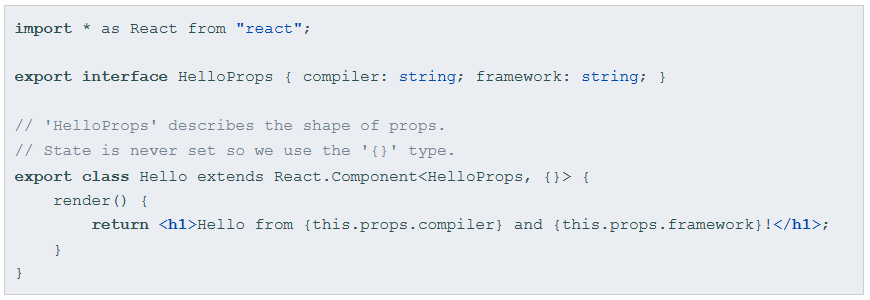
\includegraphics[scale=0.5]{react_typescript_example}
	\label{fig:reacttypescriptexample}
\end{figure}

Dynamically typed languages are a liability to the stability of our eventual product. Our frontend website must be able to stand the test of time without unnecessary downtime or fatal bugs that might interrupt the workflow of our eventual users. Our team will not be around to perform maintenance on the archive frontend after we have long since graduated. Thus, in order to reduce the chance that another senior design time will have to come in and clean up our mess, we are avoiding the dynamically typed language JavaScript. We did not make this decision lightly. It is obvious that JavaScript is the industry standard for interactive websites. However, we believe that we will see better stability by supplanting its use via TypeScript.

Typed languages eliminate an entire class of bugs and reduces the frequency of run-time crashes. Research performed by Zhang Gao \textit{et al.} at The University Collage London and Microsoft demonstrated that the use of TypeScript enables developers to reduce the number of bugs by approximately 15\%.\cite{typescriptpaper} They examined the commit history of several open source JavaScript applications. The identified the commits that corresponded to the introduction of a bug. Then, they would leverage TypeScript by adding type annotations to the code in question. If the newly annotated code prevented the bug at compile-time, then they determined that TypeScript would have prevented said bug from ever causing an issue in the first place. Of the 400 public bugs that they examined, TypeScript was able to prevent 58 bugs from occurring due to type checks at compile-time. Their conclusions are really and understatement on the impact of strict typing. They only examined public bugs and thus they did not account for bugs that were caught by developers manually during the development process. Likewise, strict typing also impacts the quality of the tools surrounding a language. Simple tasks in code navigation suchas "go to definition" and "see usages" are substantially improved by strict typing. Similarly, strict typing can reduce developer confusion since the arguments to a function or method include additional information beyond simply their name. i.e. the types associated with the arguments passed to the method in question. The results of the Zhang Gao paper was a huge motivating factor for our team. We are not expert frontend developers and thus we benefit from the additional power that TypeScript brings during the tooling process.

\subsection*{Extended Frontend Research}

Before we can begin planning the structure of our frontend code, we must first take a closer look at the way that React applications are built. This section examines many of React's idioms, components, props, application state, application life-cycle, and fillable web forms. Understanding how each of these elements make-up a React application will give our team the groundwork to begin creating our own React application for use in the archive system. It is vital that our team has a good understand of how a React application functions before we begin implementation due to our constrained timeline. Likewise, utilizing React idioms appropriately will ensure that future senior design students who might maintain or extend our code will be able to have an appropriate starting point for their project. The last thing that our team wants is to deliver a project that will just have to be scrapped and rewritten if/when any future maintenance is needed.

\subsubsection*{A Closer Examination of React Components}

Components are the main way in which one structures a React application. As mentioned above, components are React's way of compartmentalizing reusable pieces of one's design. They can be structured as side-effect free functions or as classes which extend the \texttt{React.Component} super-class.

Functional components are a good way of structuring simple components. They fit when a component doesn't have a need for child components or if its child components don't have a need to access the parent's props. Figure \ref{fig:reactfunctionalcomponent} shows a simple React functional component.\cite{reactcomponentsandprops} React automatically calls the function as needed when the associated prop data changes. This leads to very efficient rendering and simple code structure.

\begin{figure}[h]
	\centering
	\caption{React Functional Component}
	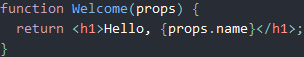
\includegraphics[scale=0.5]{react_functional_component}
	\label{fig:reactfunctionalcomponent}
\end{figure}

Class components are the heavy lifters in the React framework and typically make up the majority of the components implemented. The class components enable the developer to encapsulate the functionality of a piece of the web application to ensure that it is reusable. Likewise, utilizing class components keeps all of the necessary data associated with the markup being rendered. This structure ensures that any callbacks such as \texttt{onClick} can be swapped out since they can reference the properties of the encapsulating class. Click handlers can by dynamically assigned depending on the application's current context. This flexibility enables the developer to write generic components which can be reused and repurposed.

\begin{figure}[h]
	\centering
	\caption{React Functional Component}
	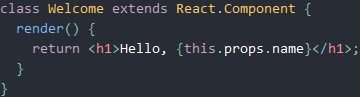
\includegraphics[scale=0.5]{react_class_component}
	\label{fig:reactclasscomponent}
\end{figure}

\subsubsection*{How React Handles State}

React handles state via prop objects. Props are arbitrary inputs that are passed to React components at run-time. The data contained within said props is the used to update the display to the end-user. Figure \ref{fig:reactstateexample} demonstrates the unintuitive what that React handles state during the lifetime of its components. Yet, this way of handling state is what makes React so powerful.

\begin{figure}[h]
	\centering
	\caption{React State Example}
	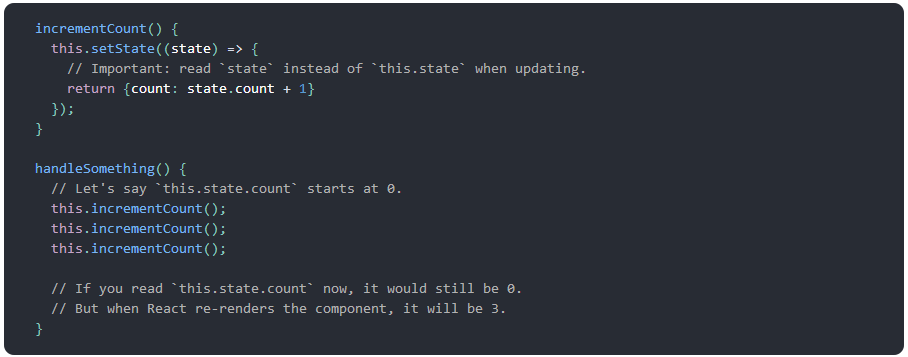
\includegraphics[scale=0.5]{react_state_example}
	\label{fig:reactstateexample}
\end{figure}

Props are read-only and cannot be directly modified. This invariant is not enforced by the library and must be strictly adhered to by the developer. Direct modifications to a prop can cause very strange behavior and possible bugs or even crashes. Instead of direct modification, props are updated via the \texttt{setState} method. This method is inherited from the \texttt{React.Component} super-class that all React components must inherit from. Utilizing \texttt{setState} instead of direct modification enables React to update the browser Document Object Model (DOM) lazily. This lazy update technique is at the core of what makes React a fast and efficient framework.

Frontend applications are asynchronous by nature and React is designed to accommodate async behavior by its very nature. Frontend applications must utilize async methods to ensure that the user experience is unaffected by long-running tasks such as network calls. There are many methods of accomplishing asynchronous dispatch but React is equipped to handle any of them provided that they adhere to the state invariants that React mandates. The \texttt{setState} method mentioned above enables React to accept statue updates from async sources and update the visual DOM efficiently. The \texttt{setState} method can merge several state updates into the existing component state in a batch fashion. Like the other React design decisions, the asynchronous allowances provided by the \texttt{setState} method are done for the state of efficiency and lazy evaluation.

Data in a React application always flows down. Parent components are able to update the state of their children. However, the reverse is not true. This unidirectional flow invariant also contributes to the lazy update technique discussed above. By ensuring that the data only flows in one direction, React can eliminate the need to update entire branches of the DOM.

React components are unable to tell if their children are stateful or stateless. i.e. class components or functional components. This separation of concerns contributes to the modularity of React components. Data is passed from parent to child and since data modifications are only performed via prop updates components can be refactored without great difficulty.

\subsubsection*{Asynchronous Data Fetching}

In order to build applications that feel responsive, asynchronous HTTP requests are a necessity. Executing requests on the rendering thread is a surefire way to make one's application feel sluggish given the nature of computer networking. Users are accustomed to instant feedback for their actions. As previously mentioned, React is quite happy to accept updates from asynchronous sources. However, like the other technologies examined, industry has moved away from utilizing plain JavaScript to handle HTTP requests. It is perfectly viable to perform said requests in plain JavaScript but there a plenty of libraries which exist to simplify the process and reduce the chance for errors. We briefly examined three methods of executing HTTP requests: plain JavaScript, the Request library, and the Axios library.

Utilizing plain JavaScript for HTTP requests cannot be overlooked. Our project will need to make simple HTTP REST requests. JavaScript is perfectly capable of handling said requests without any additional library requirements. Given that our project might need to maintained by other individuals or students in years to come, it would behoove us to attempt to minimize the number of libraries that must be learned before they can get started making modifications. Figure \ref{fig:javascripthttprequest} shows a simple HTTP request snippet provided by the Mozilla developer documents.\cite{mozillahttprequest} The aforementioned snippet shows that JavaScript is perfectly capable of making asynchronous requests in an idiomatic way. The developer just needs to declare anonymous functions to handle the callbacks which will be fired when the request completes.

\begin{figure}[h]
	\centering
	\caption{Plain JavaScript HTTP Request}
	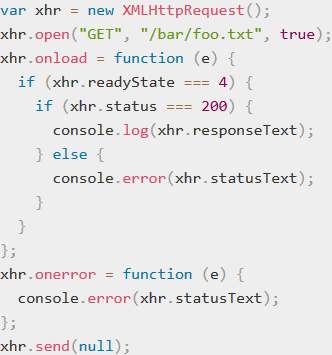
\includegraphics[scale=0.5]{javascript_http_request}
	\label{fig:javascripthttprequest}
\end{figure}

Request is a popular JavaScript library for handling HTTP requests in a simplified manner. It condenses the verbose syntax required for plain JavaScript HTTP requests into a specialized set of functions with sane defaults. Some such convenient helper methods are: \texttt{request.get()}, \texttt{request.post()}, \texttt{request.put()}, etc. Since HTTP request code is repeated in several places, it is beneficial for a developer to utilize a library with a clean and friendly syntax to reduce the chance that a mistake will be made when constructing the HTTP request code.

\begin{figure}[h]
	\centering
	\caption{An Example of the Axios Library Usage}
	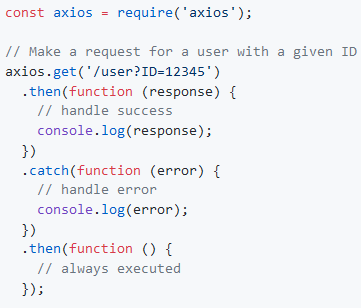
\includegraphics[scale=0.5]{axios_example}
	\label{fig:axiosexample}
\end{figure}

Axios is another well known JavaScript HTTP client library that seeks to simplify the process of making HTTP requests. However, unlike Request, Axios puts a focus on utilizing the promise API to manage its connection responses. Thus it requires a modern version of JavaScript (ES6+) in order to function. However, despite this limitation, the resultant code one writes when using Axios ends up being very clean and understandable. Figure \ref{fig:axiosexample} shows an example of utilizing the Axios API to make a basic GET request corresponding to a specific userID.\cite{axiosgithub} The example code provided shows the power of chaining several Axios methods together. The example code is very readable and mirrors the structure of natural language instructions. Structuring code in this way helps to reduce the cognitive load on the developer. This leads to better code and faster code reviews since it is easier to explain to other developers what each method call accomplishes.

\subsection*{Frontend Design}

In order for our archive to be actually useful, it must be more accessible and specialized than a simple file browser. It must serve the needs of the individual researchers at the observatory and simplify their workflow in order to magnify their productivity. Thus we will utilize the metadata contained within the Flexible Image Transport System (FITS) file format. In doing so, we will enable the researchers to search and categorize data without the need of opening individual files to inspect the associated metadata.

The Flexible Image Transport System (FITS) file format is a well known file format in the astronomy community. Much of the data generated by observatories are contained within FITS files. Our research indicates that there are many open source libraries for interacting with FITS files. However, native file browsers lack access to much of the data contained within. Thus, searching for and organizing the data is constrained by the native file browser's limitations. We seek to extricate the metadata out of the individual FITS files and create a database that can be queried for the metadata in a dynamic way. The archive frontend will need to utilize the backend API to display the metadata to the end user as they browse the archive's contents. By organizing our application in this way, we minimize the amount of data that needs to be sent by the server since not all of the metadata is needed in order to display the files as one browses the archive's contents.

Figure \ref{fig:frontendmockup} shows a mock-up of the archive's homepage. It will serve as the hub for browsing the archive's contents. The decision to display data on the homepage reflects our commitment to simplifying the access to the observatory's data. As previously mentioned, it is vital that researcher's have quick access to the data contained within the archive. Our hope is that the archive website becomes an invaluable part of their daily workflow. Navigating through a user interface before one even gains access to the data is counter-productive to that end goal.

\begin{figure}[h]
	\centering
	\caption{Mock-up of the Primary Frontend Homepage}
	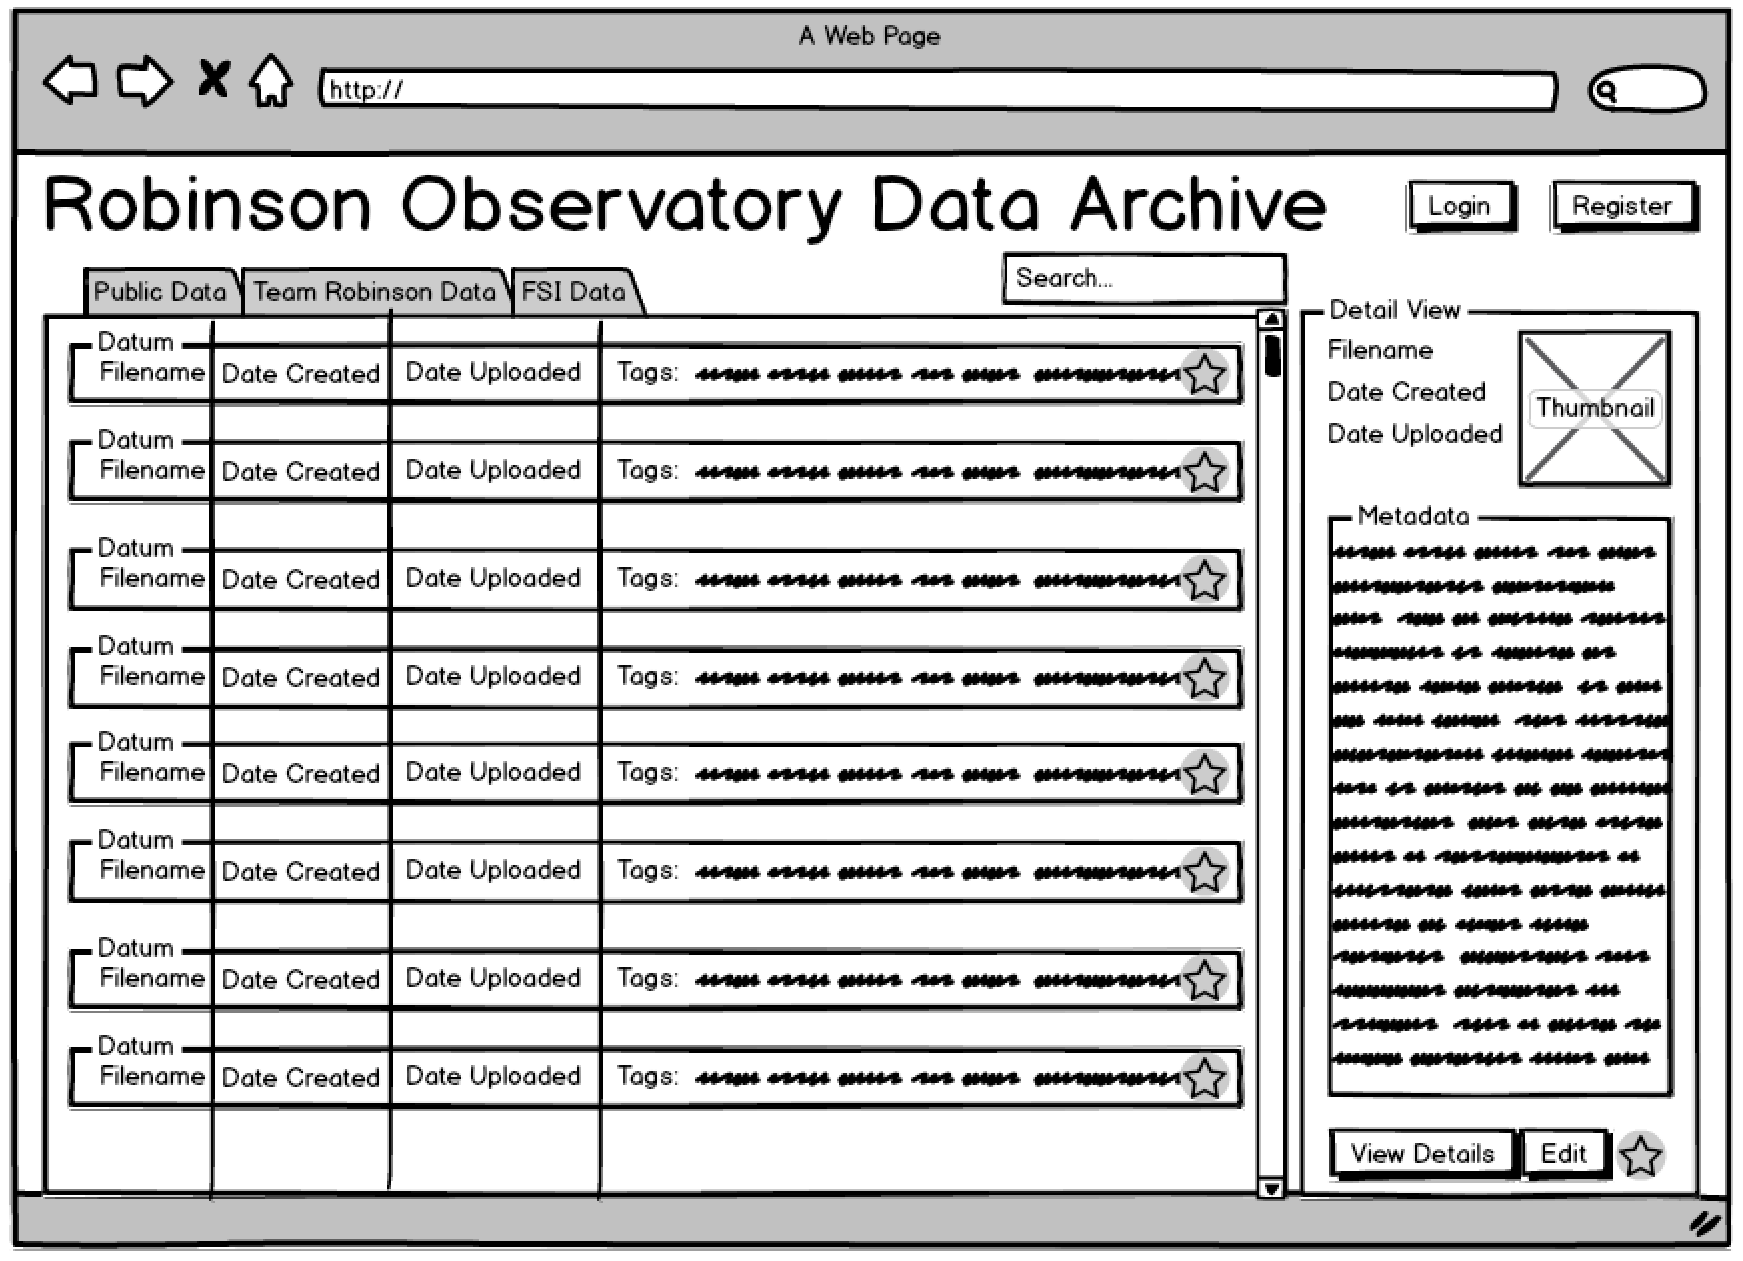
\includegraphics[width=\linewidth]{frontend_mockup}
	\label{fig:frontendmockup}
\end{figure}

\subsubsection*{Login and Registration}

One of our stated goals for the archive is open access to members of the public and potential external researchers. However, there is the possibility that access to some data will need to be restricted to outside individuals. Thus, we are forced to implement authentication as part of our design.

Figure \ref{fig:loginmockup} shows our idea for a login prompt. It is minimalistic by design. A simple prompt for username and password is all that is required for our use-case. Not pictured here is a similar registration window that would add a confirm password prompt and an organization selection box. The group access selection is needed because individuals might belong to organizations that have individual access policies. Likewise, the data associated with each organization would be potentially restricted to members of that individual organization.

\begin{figure}[h]
	\centering
	\caption{Login Mock-up}
	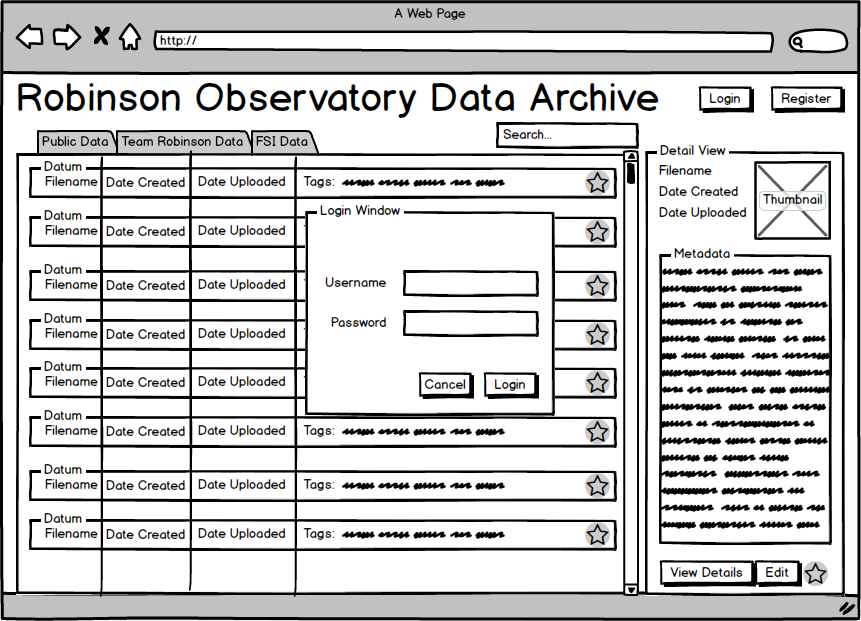
\includegraphics[width=\linewidth]{login}
	\label{fig:loginmockup}
\end{figure}

Membership to an organization needs manual approval by an administrator account that belongs to said organization.

% TODO add picture for admin queue

\subsubsection*{The Archive's Splash Screen}

Displaying data as the first thing that one sees may be initially jarring to someone unaccustomed to the website. Thus, it may be prudent to display a splash screen message when one visits the website for the first time. This would serve to ease the user into the system and help to prevent them from being overwhelmed with options. Such a splash screen would then be disabled upon subsequent visits to the archive. Figure \ref{fig:splashscreenmockup} shows our initial designs for a splash screen that would be displayed to first time visitors.

\begin{figure}[h]
	\centering
	\caption{Mock-up of the Welcome Splash Screen}
	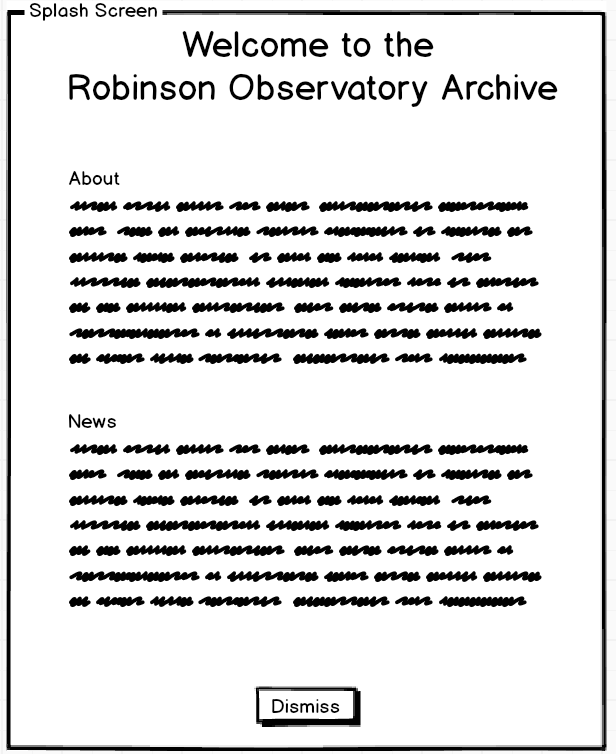
\includegraphics[scale=0.5]{splash_screen_mockup}
	\label{fig:splashscreenmockup}
\end{figure}

The splash screen would explain details about the archive's purpose and information about the observatory in the about section. We want the about section to answer questions that both the public might have and information that would be useful for researchers. Thus it is vitally important that the information contained within the about section is sourced from both researchers and unprejudiced members of the general public. We will need to interview researchers and the public in order to construct the about section's content. It is vital that this portion of the website is well constructed since it is very likely that it will be the first thing that a user reads upon visiting the archive. First impressions are vital to user engagement. A potential spelling or grammar mistake in this section could color a user's impression about the archive in a very lasting and impactful way.

Another section of the splash screen could display news about community outreach projects that the Robinson Observatory team are currently involved in. Likewise, the news section can contain links to said information so that first time visitors are exposed to the other websites that the Robinson Observatory maintains. This would also help to mitigate the impact on users that potentially stumble on the archive unintentionally. It would provide them with a convenient escape-hatch which would take them back to the "friendlier" (i.e. community focused) portions of the observatory's web-presence. This section is tightly connected to the about section since it is also might be the first thing that one reads in the archive. However, since it is the second thing displayed, readers are likely to be somewhat engaged if they stuck around to get to this section. Thus it is possible for use to include potentially denser content since the fact that they are reading the section means that they are more interested than the casual visitor might be.

\subsubsection*{The File Browser}

Once the user dismisses the splash screen, they are presented with the primary interface. As previously mentioned, Figure \ref{fig:frontendmockup} shows the general layout of the archive home page and figure \ref{fig:frontendfilebrowser} shows the file browser component of the main screen. The left-hand side of the page will display the the data which has been uploaded to the archive. Internally, we have been referring to this section as the \textit{file browser}. It will function similarly to a standard operating system file browser. However, it will be augmented with the capacity to sort and search based on the FITS file format metadata. Likewise, we want to be able to support custom tags which will simplify the process of working with the data during research.

\begin{figure}[h]
	\centering
	\caption{The File Browser Component of the Main Screen}
	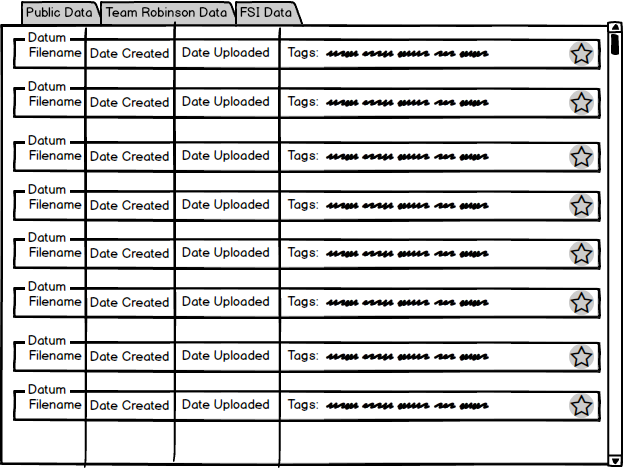
\includegraphics[scale=0.5]{frontend_file_browser}
	\label{fig:frontendfilebrowser}
\end{figure}

The file browser will need to be paginated due to the high likelihood that there will be a large number of files uploaded to the archive. Downloading an entire list during each visit would be unnecessarily bandwidth intensive. There are two approaches that we have considered and will need to be experimented with as we begin implementation. The first is a standard pager layout with arrows at the top/bottom of the file browser window. This will enable the end-user to move along as they exhaust their search. This approach is practical and familiar to the average user. Likewise, this is the strategy that Google utilizes for their search queries. (The fact that Google uses this for their interface is a good indication that we should utilize this approach.) Another alternative is to dynamically load new data as the user scrolls in an attempt to make the scrolling as seamless as possible. However, this strategy comes with a fair amount of additional technical requirements. The client must be able to detect which direction that a user is scrolling and dynamically cache the required information in the browser. This is a complex technique that would add a significant amount of difficulty to our implementation. However, if done properly, it would significantly increase the satisfaction and usability of our archive frontend. It would help to convince the end-user that the data is immediately available and it would help to reduce the perception that the data is stored on an external server. It is our belief that making the data seem like it is immediately available will increase the likelihood that a researcher would be satisfied while utilizing our archive. Any perceived delay might cause a potential user to manually cache the files that they are working with. We want to discourage such a practice by making our archive workflow as seamless as possible.

\subsubsection*{The File Preview}

Navigation of the archive is only one aspect of the archive. The second and perhaps more obvious aspect is the need to view the files directly. Research cannot be performed on the data if it is unable to be viewed. Thus we need to be able to display the data within the archive as the end-user searches. We have explored several options for displaying the data as one performs the search.

The first, and perhaps most obvious option for displaying the data, is to enable the end-user to navigate to a details page upon selection of an entry in the file browser. However, this strategy is somewhat counterproductive to our goal of simplifying the user's workflow. Switching context as one searches would interrupt one's thought process. It would be akin to going into another room when one turns the page in a book. Each file inspection would not only switch the context of the web-browser but also the context of the end-user's brain. There is a reason that integrated development environments (IDEs) have so many sub-views displayed on screen at the same time. Switching context inherently interrupts one's thought process. Another aspect to consider is the preservation of application state between context switching. As previously mentioned, we plan on utilizing React as our frontend framework. It is quite possible that, given React's nature as a "single-page frontend framework", we will have to implement some additional logic to ensure that the end-user is able to return to the exact scroll-position upon navigating back from the aforementioned context switch. This additional complexity might save memory on low end computers since we would be serializing the state to disk but this advantage seems somewhat negligible in the face of additional complex code requirements. Thus, this option is unappealing despite its conceptually simple nature.

The second option that we explored for displaying the contents of each file is a always visible file preview sidebar. Figure \ref{fig:frontendfilepreview} demonstrates this design of the preview browser display. It is always visible and serves to display the contents about the currently selected file as one scrolls through all files in the archive. This approach ensures that the user's workflow is not interrupted by a switch in context. The pertinent data is always displayed on screen and so the user only needs to look to the side to determine if it is the file that they are looking for. The obvious downside to this approach is that screen real estate is always a concern when one is designing a user interface. Smaller screens will need to be able to display the maximum amount of data on the screen at a time. Likewise, this approach would severely hamper our ability to display the archive on mobile browsers. It is very likely that the file preview would come to dominate the entire screen on such devices. This would mean that our archive would either be unsuitable for mobile devices (an unattractive proposition since one of our stated goals is accessibility) or we would need to adapt our design to remove the preview sidebar when it detects a small display. The latter is an attractive option and would been potentially easy to implement. However, a loss of functionality, no matter how necessary, is something to be lamented. Yet trade-offs must be made and we suspect that mobile users are willing to accept said trade-offs provided that they have access to the requisite data. Thus, the file preview sidebar is a very attractive option for our purposes.

\begin{figure}[h]
	\centering
	\caption{The File Preview Component of the Main Screen}
	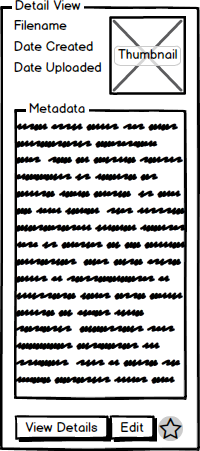
\includegraphics[scale=0.5]{frontend_file_preview}
	\label{fig:frontendfilepreview}
\end{figure}

The final option that our team has explored is a floating detail display view. Figure \ref{fig:frontendfloating} demonstrates this alternative layout as a modification on Figure \ref{fig:frontendmockup}. This option is something of a middle ground between the two prior options.

Upon selecting a file to preview. The floating view would be presented to the user in the foreground of the current display. Elements from the active file browser would still be visible but partially obscured by the floating view. This would mean that current context would not be entirely lost by navigating to a new page entirely. Likewise, as previously mentioned, the end-users brain context would not be completely lost by a complete swap in visual information.

The new information would be "anchored" by the prior view in the background. The extra screen real estate taken up by the floating view would mean that would be able to display more of the data's metadata on screen at a time. This would reduce the need for a scroll-bar attached to the metadata section. It is still possible that one will be required depending on the quantity of metadata present. However, displaying more at a time would imply that the user could find what they are looking for more quickly. In total, this display strategy would hopefully mean that the inspection of files would be a rapid process and that the archive's usability would be greatly augmented by utilizing this strategy.

\begin{figure}[h]
	\centering
	\caption{An Alternative Mock-up of the Primary Frontend Homepage}
	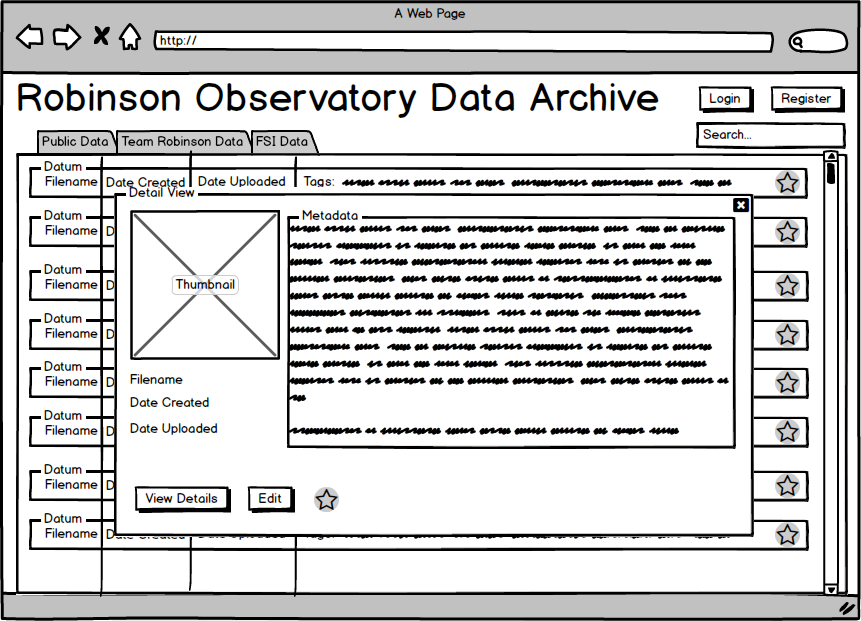
\includegraphics[width=\linewidth]{frontend_floating}
	\label{fig:frontendfloating}
\end{figure}

The display technique is familiar to most modern users. Many modern websites and native applications utilize floating windows to great effect. Likewise, floating components have become a vital part of mobile applications. Thus, users have been trained to understand how this kind of display component behaves.

\section*{Database Research}

\subsection*{SQL vs NoSQL}

\subsubsection*{SQL}

Structured Query Language (SQL) is the most popular language for managing Relational Database Management System (RDBMS).  SQL was initially developed by IBM researchers Raymond Boyce and Donald Chamberlin in the 1970s.  SQL includes data query, data manipulation (insert, update, and delete), data definition, and data access control.  SQL is known for its readability and ease of learning.  MySQL and Microsoft SQL Server are two widely used database systems each being used for LAMP stacks and WISA stacks respectively.  Just recently, both options have become available on Windows, Linux, and MAC OS X.  Due to its age and availability, SQL is heavily documented in its functionality.

\begin{figure}[h]
	\centering
	\includegraphics[width=0.251\linewidth]{mysql}
\end{figure}

\subsubsection*{MySQL}

MySQL is an open source Relational Database Management System (RDBMS) that uses Structured Query Language (SQL).  MySQL is the database component of the LAMP (Linux, Apache, MySQL, PHP) web application software stack.  MySQL is used by popular companies such as Netflix, NASA, Tesla, and Youtube.  MySQL was created by a Swedish company, MySQL AB, by David Axmark and Michael Widenius in 1995 and is currently owned by Oracle.  Similar to SQL itself due to the age of MySQL, its complexity and problems have been encountered and documented so solutions are readily available.  The popularity of MySQL creates a loop of being popular due to its popularity.  Developers are readily available and the cheap hosting environments makes MySQL very accessible.  It is primarily written in C and C++.  While still open source under Oracle, some modules are proprietary and close-sourced.

\begin{figure}[h]
	\centering
	\includegraphics[width=0.251\linewidth]{microsoftsql}
\end{figure}

\subsubsection*{Microsoft SQL Server}

SQL server is owned by Microsoft and has frequent releases.  The licenses required for running SQL server makes it more expensive than MySQL which is free and open-source outside of the enterprise level.  SQL server is mainly used in Microsoft’s WISA (Windows, IIS, SQL Server, ASP.NET) stacks where all components were designed by Microsoft and built to function together.  The added benefit of WISA stacks is that customer support can be handled by Microsoft across all levels.  SQL server is very to install and has transparent data compression and encryption which also provides better security features.

\subsubsection*{NoSQL}

A database technology that does not involve the structured query language and rely on object-oriented APIs instead.  NoSQL contains various database types mainly including document databases, graph stores, key-value stores, and wide-column stores.  A document database will pair a key with a complex data structure known as a document.  Graph stores store data based on networks of data e.g. social connections.  Key-value stores store every single item as an attribute name along with its value.  Wide-column stores make use of columns of data, rather than rows.  NoSQL provides a more scalable platform and improved performance.  The various structures of data storage and management alongside cloud development were key features of NoSQL that SQL did not anticipate.
NoSQL provide dynamic schemas rather than the strict requirements of relational databases.  Adding additional information requirements in relational databases require downtime in shifting all of the previous information to the new tables.  NoSQL and lack of table structure provides flexibility that is unseen in relational databases.  When not all specifications are known or explored in advance, NoSQL is able to add additional data requirements more easily.  NoSQL is developed with cloud storage in mind and is able to easily make use of cloud data storage whereas relational database systems do not support this natively.
NoSQL Databases are a newer technology from the late 2000s that were developed specifically to combat the limitations of SQL databases, mainly scalability, multi-structured data, geo-distribution, and agile development.  NoSQL databases are widely more dynamic and flexible than SQL databases and remain open source.

\subsection*{SQL Alternatives}

\begin{figure}[h]
	\centering
	\includegraphics[width=0.251\linewidth]{mariadb}
\end{figure}

\subsubsection*{MariaDB}

MariaDB was created by MySQL founder Michael Widenius when Oracle obtained MySQL in 2010 and stays true to its open source, community driven development.  MariaDB is a direct alternative to MySQL and is a fork of MySQL.  The functionality is similar enough that MariaDB functions as a database as a drop-in replacement for MySQL.  The database structure and indexes are the same as MySQL.  MariaDB is used by companies such as Google, Wikipedia, RedHat, etc.  The main advantages of MariaDB despite being a fork is its more efficient performance and newer features.

\begin{figure}[h]
	\centering
	\includegraphics[width=0.251\linewidth]{postgresql}
\end{figure}

\subsubsection*{PostgreSQL}

PostgreSQL is another open source SQL database but it is object-relational.  Object-relational means that there is support for user-defined objects and their behaviors e.g. data types, functions, operators, domains, and indexes.  Alongside these objects, PostgreSQL has a wide support for data types and structures.  PostgreSQL can store much more data in their rows without negatively impacted performance.  MySQL and MariaDB are known for running into file size limitations and PostgreSQL will avoid those problems.  The highly customizable databases and wide support for programming languages are some key features of PostgreSQL.  PostgreSQL is widely used and well-known for data stability and security.  PostgreSQL combines the benefits of SQL with the modern features of noSQL and looks to be very promising.

\begin{figure}[h]
	\centering
	\includegraphics[width=0.251\linewidth]{mongodb}
\end{figure}

\subsubsection*{MongoDB}

MongoDB is the database component of the MEAN (mongoDB, Express, Angular, Node.js) and is a NoSQL database.  MongoDB is based in JavaScript alongside the entire MEAN web-based application stack.  MongoDB was developed in 2007 and introduced to the market in 2009 as an open source database that was maintained and supported by MongoDB Inc.  MongoDB utilizes JSON based document oriented queries that function much more quickly than SQL queries.  NoSQL databases are a more modern approach to databases and mongoDB is in the forefront.  In terms of modernity and future web stack development, mongoDB seems like the most flexible choice for databases.

\begin{figure}[h]
	\centering
	\includegraphics[width=0.251\linewidth]{dynamodb}
\end{figure}

\subsection{DynamoDB}

DynamoDB is a noSQL database developed by Amazon.  DynamoDB makes use of tables, items, and attributes and seems to have a much more simplified query calls for a noSQL database as compared to mongoDB.  In line with the Amazon brand, the database is designed with scalability in mind and offers a wide variety of features if chosen alongside with Amazon Web Services.  DynamoDB seems like an interesting option for a noSQL database.

\section*{Backend Research}

The main component for communication between the front-end user experience and the database itself is the backend.  The server-side functionality of retrieving and storing data as requested by users into the database and other various API function calls is the job of the backend.  The backend mainly consists of the servers, databases, APIs, and operating systems.

\begin{figure}[h]
	\centering
	\includegraphics[width=0.251\linewidth]{php}
\end{figure}

\subsection*{PHP}

PHP began development in 1994 by Rasmus Lerdorf.   PHP is a general-purpose programming language designed for web development and can be easily embedded into HTML.  The PHP code is executed server side which will send the corresponding html to the client and these actions are fully synchronous.  Issues related to synchronous behaviors offer some drawbacks as web application development begins to evolve towards asynchronous behaviors.  From personal experience it is somewhat intuitive and relatively streamlined and template based.  Within the PHP code, a connection to the database will be made, a SQL query will be processed from the client and the corresponding data will be sent or retrieved from the SQL database.  The connection will then be closed until the next client interaction happens.

\begin{figure}[h]
	\centering
	\includegraphics[width=0.251\linewidth]{nodejs}
\end{figure}

\subsection*{Node.js}

Node.js is an open source server environment that executes JavaScript on the server and works in conjunction with express.  Node.js differs from PHP as it makes use of asynchronous programming.  Asynchronous programming makes Node.js much more efficient as it is able to send requests and immediately prepare other requests rather than waiting after every single request.  As soon as a request is ready, the contents will be sent to the client rather than waiting for the request to be fulfilled.  The MEAN stack of Node.js will make use of JavaScript across the stack which will provide easier communication across the levels of the stack between developers.  This aspect will be particularly useful in the scope of this project as there are very few of us and communication and ease of troubleshooting is extremely important.

Node.js and the MEAN stack in general is not as mature as technologies as PHP and the LAMP stack but their more modern approach to web development is very promising and the growth in popularity in the last decade is exciting.  Asynchronous calls allow for better communication on both ends with real-time connections and better data exchange.

\begin{figure}[h]
	\centering
	\includegraphics[width=0.251\linewidth]{express}
\end{figure}

\subsection*{Express}

Express is a lightweight web application framework for Node.  Express is known for simplifying routing, which is how a web application’s endpoints respond to client requests.  This greatly simplifies the web application development process and eases data communication between the backend and the frontend.  Not only is the connection eased but being able to make requests and calls are simplified also because of the framework that express offers.  Node.js and Express offer a straightforward platform to developing a web application backend.

\begin{figure}[h]
	\centering
	\includegraphics[width=0.251\linewidth]{aspnet}
\end{figure}

\subsection*{ASP.NET}

ASP.NET is a combination of Active Server Pages (ASP) and .Net Framework.  ASP is Microsoft’s scripting engine for dynamic web pages and .NET is the software that enables use of ASP.  ASP.NET is part of the WISA stack.  The closed source aspect of being a Microsoft product can be a drawback.  WISA stacks and the prices associated seem to be mainly targeting enterprise level websites however when using WISA stacks, all levels of the stack can be handled by Microsoft support which would smooth any issues with the web application.  The Visual Studio IDE also assist in the web development step with the various features available with the C\# language.

\begin{figure}[h]
	\centering
	\includegraphics[width=0.251\linewidth]{rubyonrails}
\end{figure}

\subsection*{Ruby on Rails}

Ruby on Rails is a server-side web application framework written in Ruby under MIT license.  Rails provides a model-view-controller (MVC) framework and structures for a database, web service, and web pages.  The frameworks provide a platform and templates for developing websites.  The process with rails seems to simplify the coding process similar to design patterns by providing efficient and clean solutions to common issues or specifications in web application development.  Ruby on Rails sounds like a user-friendly option that could be worth exploring although learning ruby alongside the framework seems like a unique experience.

\section*{Web Hosting}

The current website for the Robinson Observatory is currently maintained by the astronomer team and is apart of the UCF website domain.  This will give us flexibility in what features will be added as the website is directly handled by those that maintain it.  While working on the future additions to the website, we will host a website on our own service for ease of access when developing and making changes as progress is made.  Image hosting and associated data will be a large component of the website as the data the observatory has previously stored is already over 100GB.  We will likely utilize a subset of the data until we are confident in our abilities to manage the data to our needs.  Data storage and security will be a requirement to keep in mind.  Cloud services and scalability will be a factor to keep in mind to keep the service modern and functional as the scale of the service grows with more image and data capacity.  The possibility of machine learning being a functionality will also increase storage space dramatically due to requiring a large pool of sample images in order to be able to correctly and accurately train a system to recognize images properly.

\subsection*{Web Host Options}

The big three website hosting services are AWS, DigitalOcean, and Google Cloud.  In terms of cost and user-friendly experience in setting up a service, All the options seem very similar.  DigitalOcean seems to be the most affordable choice alongside with the medium-scale demonstration size of the website for this project will be, however AWS and Google Cloud offer extensive documentation in their domains.  AWS offers a wide variety of services in their field that is capable of deploying a database, website, and storage all from an amazon account.  The contained functionality of the many services offered can be seen as an appealing feature.  All these options offer special deals and credits for students and should all be affordable in terms of support for the next year until our website functionalities are integrated to the robinson observatory website.

The senior design lab also offers server space and hosting.  The main issue is requiring a VPN when not on campus to edit the files and update the website.  One of the web hosting services seems to be the simplest option and all options are affordable without requiring VPN access.


\begin{figure}[h]
	\centering
	\includegraphics[width=0.251\linewidth]{aws}
\end{figure}

\subsection*{Amazon Web Services (AWS)}

Amazon Web Services is an extremely flexible platform with a wide variety of options for all web hosting needs.  The idea of scalability and flexibility are key aspects that AWS utilizes to meet the needs of their customers as their platforms and storage needs grow.  AWS also offers the largest amount of credits (\$185.00) specifically for student usage through the AWS Educate program.  The AWS Educate program is designed to be an academic gateway for future web services professionals.  Their goal is to raise awareness of cloud services and their capabilities.
Another draw to AWS on top of their flexibility and scalability of creating your database and website is their extremely useful and resourceful documentation.  All components of a website are offered by Amazon Web Services from the domain name to databases to the website itself and everything is documented.  A variety of guides to setting up a database of your chosen language whether it be a relational database such as MySQL, PostgreSQL, MariaDB, and more or it is a non-relational database such as MongoDB or Amazon DynamoDB.  The guides are created extremely thoroughly with common troubleshooting issues within their instructions to make the process as easy as possible.
The following steps of connecting your database with your chosen web platform and creating your website continues the trend of well-documented instructions.  Creating a Node.js platform and connecting the PostgreSQL was a streamlined processed thanks to the documentation and the wide variety of tools offered by AWS.  In this case their elastic beanstalk feature which is their web platform tool allows for easy connection to the database and the great scalability features that Amazon Web Services offers.

\section*{Database}

The database for the website will be using postgreSQL.  The main benefits of postgreSQL is that it is an open-source object-oriented relational database that can also feature noSQL functionalities.  PostgreSQL is also known for its dependable data storage and security.  The databases main feature will be the images of the telescope.  Filepaths to images will be stored in a table and be associated with corresponding metadata.  The metadata table will make use of postgreSQL’s functionality to create self-made array types to store the metadata of each subsection together.  Users will be able to create accounts with some personal information associated and be able to create tags for photos and favorite them.  There will also be a public and administrator level to account types that will allow the general public to view and interact with the images whereas an administrator account would be able to edit metadata or add and delete images from the database.
Below is an entity relationship diagram for our database which shows the associations between the tables and the data held within each table.  The tables seek to contain each of the main components of the database to their own tables while also being able to easily create queries to intuitively search the database and make changes as needed.

\begin{figure}[h]
	\centering
	\caption{An Entity Relationship Diagram of the Database}
	\includegraphics[width=\linewidth]{database}
	\label{fig:ERD}
\end{figure}

\begin{figure}[h]
	\centering
	\includegraphics[width=0.251\linewidth]{postgresql}
\end{figure}

\subsection*{PostgreSQL Setup}

Creating a database on Amazon Web Services proved to be extremely intuitive and simple with their extensive documentation.  Amazon offers relational database creation under a wide variety of languages and PostgreSQL is one of them.  Upon creating the database on AWS, the following step was to create the tables for the database.  This step involved the use of pgAdmin.  pgAdmin is an open-source administration and development platform for PostgreSQL.  The creation of the tables involved the use of SQL to create tables with the desired fields and their data types.  Below is an example of a table created for the database on pgAdmin.  The choice of SQL made creating the tables extremely simple with the clear syntax of the data structure and data types.  Queries are also simplified through their use of intuitive key words to form a desired search based on conditions to capture the desired subset of information.

\subsection*{Users Table}

The users table seeks to form a base for the database to form associations with images and their respective metadata.  Each user can be associated to as many images as they desire.  The users table will contain some personal information about the user for the purpose of account security but the information will not be shared or displayed publicly.  Their full name and email will only be viewable by the users themselves.  Their username will be used to log in to the website along with their password.  The passwords will be hashed using bcrypt.  Bcrypt is a long-standing and proven password hashing function designed by Niels Provos and David Mazières.  Bcrypt makes use of salt and is resistant to several variations of attacks such as a brute-force search or a rainbow table attack.  Password recovery will work through email as a form of authentication to improve account security.
A user ID will be associated with each account as a method of keeping track of accounts without any personal identification and each account will be assigned an account type.  The account type will be either public or administrator.  A public account is meant for the general public to interact with the website and view the images made available by the observatory.  A general account will be able to search the images and favorite images of their choice.  The search functionality will find the best match to their criteria based on associated tags of images assigned by administrator accounts.  The administrator accounts will involve the astronomer team and those involved with the observatory professionally.  These accounts will have special access including features such as adding and deleting images from the database and editing metadata information.
Below is an example of the SQL for the users table.


\begin{figure}[h]
	\centering
	\caption{SQL Example of the Users Table}
	\includegraphics[width=\linewidth]{database_user_table}
	\label{fig:SQL Users Table}
\end{figure}

\subsection*{Images Table}

The images table will associate images to their metadata and users can associate themselves to multiple images.  Each user can be associated to many images and each image will be associated to a specific metadata.  The images will make use of a user ID and an image ID to associate images with users in cases such as when they favorite an image or if they uploaded the image to the database.  The images themselves won’t be stored directly on the database but their file paths will be stored on the database to reduce personal data storage requirements and rely on the use of cloud storage.  Tags will be created for images in order for them to be identifiable. Tags such as “full moon”, “Polaris”, “the north star” will assist the search functionality of the database to make the website and images more accessible and increase community interactions.  A favorite functionality will also allow for images to be associated to users in a personal gallery of favorited images from the observatory.  Below is an example of the SQL for the images table.

\begin{figure}[h]
	\centering
	\caption{SQL Example of the Images Table}
	\includegraphics[width=\linewidth]{database_images_table}
	\label{fig:SQL Images Table}
\end{figure}

\subsection{Metadata Table}

The metadata table will associate metadata with their respective image.  The relationship will be one-to-one as each image should have its own unique metadata.  The metadata table will hold all the pertinent fields which will be gathered through the telescope and the associated software.  The metadata gathered form the telescope software will be used to fill the metadata table.  The fields will hold varying levels of categorized information.  The creator field will hold information such as contact information for the creator including their full name, email, telephone, and address.  Any fields that are not filled out will default to an empty string.  The content field will hold information including the name of the subject, a short description, and date collected.  The observation field will include the type of telescope used, the facility where the image was capture, the light spectrum, spatial coordination, and other technical information regarding how and where the image was taken.  The publisher field will include the associated telescope and their sponsor.  The file section will include information on the file type of the image and the size of the image.  Below is an example of the SQL for the metadata table.

\begin{figure}[h]
	\centering
	\caption{SQL Example of the Metadata Table}
	\includegraphics[width=\linewidth]{database_metadata_table}
	\label{fig:SQL Metadata Table}
\end{figure}

\subsection{Astronomical Visualization Metadata}

For every image taken at the Robinson Observatory, the telescope software is able to provide a standardized set of information about the image which is stored in associated metadata.  This standard metadata is known as the astronomical visualization metadata (AVM) standard.  The standard is recognized by the international virtual observatory alliance (IVOA) which is a worldwide scientific organization that facilitates international collaboration for access to data gathered by observatories around the world.  With this standard in place, accessing and associating metadata for our website will be much simpler.  The required fields for the database will be well defined in accordance to the AVM standard.
The AVM standard can be broken down into five separate categories: creator, content, observation, publisher, and file.  The creator category contains information about the person who created the image and how to contact them.  The content section is the title of the astronomical object with short description and some general information such as the type of the object.  The observation section holds the spatial information and coordinates, the section of the light spectrum used, and additional information for its location in space.  The publisher information is the institution associated with the observatory and how to contact.  The file metadata holds information about the image such as file type and size.
The image below contains the AVM standard with format type and examples.

\newpage

\begin{figure}[h]
	\centering
	\caption{AVM Tags Standard with Examples}
	\includegraphics[width=\linewidth]{avm_standards}
	\label{fig:AVM Standards}
\end{figure}

\section*{Archive Backend}

The back-end will make use of node.js and express to keep JavaScript across the stack.  The benefits besides maintaining a single language which will make testing and communication easier on our team also include its lightweight and efficient performance alongside the ease of use with express being a framework within the node environment.  Express will make creating the API much simpler and easier.  Typescript will also be used over JavaScript for the benefits of easier to code and avoid errors in the code that could lead to issues.
One of the main features will be account creation and logging into the account for users to be able to have their own library of images and their own favorites.  The ability to search and view images and create tags or favorite images will be key features of the website.  The website on the public-facing side will be used to gather interest in the images and activities at the observatory and these features hope to accomplish that goal.
The administrator side of the website will seek to manage the database of the images taken from the telescope.  The ability to edit metadata and to add, edit, or delete images will help to keep the database sorted while also allowing for an always accessible way to interact with the images.  The online features and cloud functionality of the website will assist in preserving the images.  These will be the main functions for the API to create a website for the images.


\subsection{Amazon Elastic Beanstalk}

Amazon offers an environment that allows for quick deployment and development of web applications through their elastic beanstalk service.  The service facilitates server management issues such as storage capacity, scaling, and monitoring and allows for simplified management of web applications to quickly deploy to the AWS cloud servers.

\subsection{Node.js Development}

Node.js offers a server-side runtime environment that enables web applications to be built quickly.  Node.js utilizes JavaScript and is an open-source, cross-platform tool.  AWS Elastic Beanstalk will offer the web hosting services and the application will utilize Node.js alongside the Express framework.

\subsubsection{Database Connection}

The first step of the backend development will involve connecting the established PostgreSQL database to the web application.  Connecting to the database requires some information from the database.  The host indicate the endpoint of the database.  The port indicates the port used for the connection.  The user and password will ensure that the access and connection to the database is valid.  In the sample code below, the PostgreSQL connection is established and the connection is tested.  If the connection fails, the console will output an error notifying the connection failed. Otherwise, the console will output a successful connection message.
Creating a Node.js platform and connecting the PostgreSQL database was a straightforward process.  Sample code provided by AWS allows for a quick preview of the capabilities of the web application and provides experience of the ease of uploading the application when needed.
The next steps will involve creating the web application involving Node.js alongside the Express framework.

\begin{figure}[h]
	\centering
	\caption{PostgreSQL Database Connection}
	\includegraphics[scale=0.5]{database_connection}
	\label{fig:javascripthttprequest}
\end{figure}

\subsection*{API Calls}

Communication between the website and the database will be handled through the backend through establishing a connection with the database as seen above and executing queries to make changes to the database based on user requests.  A query is a request for data from the tables of a database.  Keywords such as ‘CREATE’, ‘DELETE’, or ‘SELECT’ are used to add, remove, or search for data based on conditions such as matching the search using ‘WHERE’ or inserting using ‘VALUES’ followed by the data that will be entered into the database.  Queries will be the main component for the functionality of the API.  The following sections will outline a series of API calls.

\subsubsection*{Register}

Account creation will allow users to join the community and view and favorites images that they enjoy.  The process will require some personal information from the user for account security.  The sign-up process will require the user’s full name, an email, and a unique username with a secure password.  The password will be stored hashed with the bcrypt algorithm and functions to protect account security.  Below is an example query without password encryption and raw values alongside the user within the users table of the database.  All the values of the users table will be generated based on user inputs to create an account.  A row will be generated within the table on the database and their account will be created and ready to be used.

\begin{figure}[h]
	\centering
	\caption{API Example of Account Creation}
	\includegraphics[width=\linewidth]{api_raw_register}
	\label{fig:API Register}
\end{figure}

\begin{figure}[h]
	\centering
	\caption{User created on database}
	\includegraphics[width=\linewidth]{database_user}
	\label{fig:Database User}
\end{figure}

\subsubsection*{Login}

The login page will grant access to the website and the features included.  The user will be required to input their username and password which will be verified against the hashed password saved to the database.  The bcrypt library will be utilized for hashing and comparing passwords for the security of users.  If the username and password match to the values stored on the database, then the user will be logged in.  With an account a general user will gain access to being able to favorite images viewable within the web application.  Users will be able to view each other’s favorite image galleries to form a sense of community amongst fans of the observatory to share images they find exciting or unique.  Below is an example of the bcrypt hash and compare functionality.

\begin{figure}[h]
	\centering
	\caption{bcrypt Functions}
	\includegraphics[scale=0.5]{api_bcrypt}
	\label{fig:API bcrypt}
\end{figure}

\subsubsection*{Search}

The search functionality will be based on tags and return images with the matching tags.  The query will search for any tags that contain the requested value and return any matching rows within the image table.  The query will select any row from the images table where the search string is contained within the tags value of the table.  The values will then be ready as a json response for the frontend.  Below is an example query for the search functionality of the web application.

\begin{figure}[h]
	\centering
	\caption{API Example of Search Function}
	\includegraphics[scale=0.5]{api_search}
	\label{fig:API Search}
\end{figure}

\subsubsection*{Edit Metadata}

Editing metadata when required will be a key feature for the administrator level accounts.  In case any of the pre-filled metadata is incorrect or solicits corrections, this API call will make the changes based on the user requirements.  The user will be shown the metadata of the image when they want to edit and be presented with all the fields as they are in the table.  They will make their changes and save their edits which will be inserted into the table.  The query will update the metadata table by setting all values changed where the matching meta ID is.  This will minimize changes to the table by only affecting the fields that were edited.  Below is an example where the publisher is edited to the image where the meta ID is 1.

\begin{figure}[h]
	\centering
	\caption{API Example of Edit Metadata}
	\includegraphics[scale=0.5]{api_edit_metadata}
	\label{fig:API Edit Metadata}
\end{figure}

\subsubsection*{Add Favorite}

Adding favorites will allow users to collect the images they find interesting or exciting and share these specified images with others.  When adding an image to their favorites, a user will have the image ID added to their favorite column.  This will associate the image to the user and will be displayed on the user’s gallery of favorites.  The query will add the image ID to the favorites and create the association of the user and favorited image.  Below is an example of the add favorite query with fixed values.  A process to remove favorites will also be implemented for user functionality.

\begin{figure}[h]
	\centering
	\caption{API Example of Add Favorite}
	\includegraphics[scale=0.5]{api_add_favorite}
	\label{fig:API Add Favorite}
\end{figure}

\subsubsection*{Set Tags}

Tags offer a useful functionality by allowing users, whether general or administrative, to create custom ways to identify an image.  The search functionality of the website will utilize these tags when searching the database in order to identify images.  Accurate and functional tags will be an important part of the functionality of the web application and the backend.  The query will function by updating the image table and setting the tags to the specified input by the user.  A process to remove tags will also be made available in case of inaccurate or malicious tagging of images occur.  Below is an example of the create tag functionality for images with fixed inputs.

\begin{figure}[h]
	\centering
	\caption{API Example of Set Tags}
	\includegraphics[scale=0.5]{api_create_tags}
	\label{fig:API Set Tags}
\end{figure}

\begin{figure}[h]
	\centering
	\includegraphics[width=0.251\linewidth]{react_node}
\end{figure}

\subsection*{Archive Backend \& Frontend Communication}

The frontend and backend are two components of the web application that must communicate properly in order for the web application to function correctly.  The frontend specifies the user experience within the browser which will be handle by react.  The backend will interact with the database with requests from the frontend in order to manage data and either update the database or display data from the database.
The React frontend of the web application will utilize states to capture API responses and implement the required data to the user experience or ensure the correct data is sent to the backend and the database.  A react frontend will run alongside express with the use of routers functionality to share data between the react frontend and node/express backend.
The Node/Express backend of the web application will utilize SQL queries to make the changes to the database or display the requested information to the frontend.

\section*{Observatory Refreshes}

A portion of our project is some technology refreshes for some items in the observatory. The current technology is old and mostly outdated. Furthermore, some of the components at the observatory have not been used or even touched in a few years. These tasks are more IT related though than computer science and do not involve any program development or analysis.

First off, the control computer needs to be upgraded to Windows 10. It is currently running on Windows 7, which is being phased out by Microsoft. This will be achieved by first making a complete copy of the current hard drive. We run a disk imaging process through Linux on a usb stick. This will be done to ensure the current state of the control computer can be reset at any time in case of some type of failure once upgraded to Windows 10. Once updated, it will be important to ensure all drivers are fully functioning still. The control computer contains multiple drivers to control all operations of the observatory from the telescope to the dome. We will be able to run an update check on the drivers to ensure they are updated to the proper version for Windows 10 functionality. A current check has shown all drivers can function with Windows 10.

Next, the observatory faculty would like the ability to control the telescope control computer from their downstairs iMac. This feature would not only allow them to control the telescope from downstairs but also view the current progress of the telescope when it is running. To do this, the iMac hard drive will first be backed up just like when upgrading the control computer for the Windows 10 upgrade. We want the same ability to roll back the computer in case anything goes awry with dual operating systems on one machine. Then, we can install either Parallel or Bootcamp to run Windows on the iMac. Once the Windows operating system is installed, remote access to another Windows computer is feature of the operating system. Bootcamp is a feature already built into the Mac operating system but requires a reboot to switch between operating systems and the system storage options pertaining to the Windows operating side are not customizable like Parallels. When a storage size is selected at installation, it cannot be adjusted in the future like Parallels allows. This means if the Mac or Windows operating side runs out of memory, the user would not be able to adjust the memory to get more from the other operating side. Parallels runs like a virtual machine on the computer allowing the system to run Mac and Windows at the same time without the need for rebooting the computer. This can save a hassle of constant rebooting so one operating system can be used but the processing of the computer will take a toll. For the purpose of the observatory, we will use Bootcamp so Windows can be used. This decision is based on the computing power of the iMac as its an older generation and will have a hard time if running Windows and Mac concurrently. In extension, the memory customization Parallels provides would most likely go unused. The iMac is not the main operations computer of the observatory so the main memory has a large vacancy for space. Finally, Bootcamp also does not need to be purchased like Parallels does. Parallels cost \$79.99 for a one time license of the program.

Finally, the observatory has a server they want reinstated. The server was used to house all the pictures taken by the telescope and allowed for remote viewing. This update will be hard to completely test as the telescope will not be fixed during our project so we will need to send test data instead. The current server has no been used in some time and has possible water damage according to the observatory personnel. The server does boot upon testing but has yet to be hooked up to retrieve file transfers. We were able to backup their current server data to portable disk. The data we retrieved is in tact, allowing us to use their previous telescope pictures as test data within our website.

The observatory team also asked for a few more upgrades that wouldn’t be feasible for our project as they require the telescope to be in operation. They wanted scripting capabilities for their SkyX software used in controlling the telescope. This is a feature we can work into our scale model system though. Scripting is available in Stellarium as a plugin option and we can test scripting through tracking objects and viewing image data afterwards. Image data from the GoPro provides accurate timestamps allowing for precise review of the scripting success of our program(s). Our scale model will not run with SkyX but we can provide a possible overview into how it could work. They also wanted an update in the time given to the telescope picture’s metadata. It currently is given the wrong time but we have no way of producing a similar experience without the telescope working.

\section{Administrative content}

\subsection*{Budget}

\begin{figure}[h]
	\centering
	\includegraphics[width=1.0]{budgettable}
\end{figure}

\subsubsection*{Software}
The SkyX Professional Access: \$349.00 - Already Downloaded\\
Windows 10: \$140

\subsubsection*{Web \& App Development}
Web Server Hosting - AWS - use of student credits and free tier limits negate cost\\
Database - AWS - use of student credits and free tier limits negate cost

\subsubsection*{Physical Hardware}

Data storage cost for backing up the disk image - FSI provided hard drive\\
Physical Server - Observatory already has server

\newpage

\section*{Project Milestones SD1}

\begin{figure}[h]
	\centering
	\includegraphics[width=\linewidth]{SD1Gantt}
\end{figure}

\begin{figure}[h]
	\centering
	\includegraphics[width=0.6\linewidth, height=4.0cm]{SD1Dates}
\end{figure}

Senior Design 1 has a main purpose of giving us a firm foundation for what direction our project will go and how we will travel down that direction. With that being understood, much of Senior Design 1 is conceptual in nature where we are researching, designing, and testing out various avenues of attack in completing our overall project. This means that the first major goal of senior design 1 is to get a firm grasp of what our project even entails and what it is supposed to accomplish. Moving forward once we understand the project's goals, we have to then research what already exists and what does not, and then figure out how to make ours stand out while still accomplishing the overall goal. Lastly we begin testing out our ideas by setting up initial development environments and playing with basic prototyping ideas.

Looking at our gantt chart gives the overall idea behind this methodology of treating senior design 1 as our research phase. Our first milestone was the first TA check-in in February where we demonstrated what the research we had been conducting prior to then has led to, and where we plan on going moving forward. This was successful, and so then our next milestone was presenting to our senior design professor in March for a mock project presentation. In order to reach this milestone successfully, we ensured that our initial research was completed and that we had development environments set up so that we can demonstrate our understanding of initial prototype ideas to our professor and get advice and input. Again, we were successful in accomplishing this milestone and left our meeting feeling confident about the direction of our project.

Moving from the presentation, we then had the milestone of our second TA check-in in April. We wanted to have actual software and APIs to present by this point, and so we went about creating the prototypes that we talked about in the professor presentation. We accomplished this and got our initial prototypes ideas off the ground, and our TA gave us some valuable input and advice. Our last major milestone was the due date of this document at the end of April, and so we ensured that each team member had enough to work with in order to create the best design document that we can.

All of this gives us a firm foundation for our project going into the Summer and then Senior Design 2 in the Fall.

\section*{Project Milestones SD2}

\begin{figure}[h]
	\centering
	\includegraphics[width=\linewidth]{SD2Gantt}
\end{figure}

\begin{figure}[h]
	\centering
	\includegraphics[width=0.6\linewidth, height=4.0cm]{SD2Dates}
\end{figure}

Senior Design 2 is when the real work is accomplished and where the seeds of our research come to fruition. In order to accomplish this, we have to have a set-in-stone plan of action so that our team is successful at the end of the semester. Our first overall goal will be to have a fully working prototype of each piece of the project completed by September. This is because our project works with two other senior design teams, the electrical team and the mechanical team, and we have to ensure that our products work with theirs in order to actually have a working model telescope and software.

This leads into our next major milestone of being fully integrated with the other two teams products by the end of September so that all future testing and implementation can be done as an entire unit and not three separate teams. We will spend the following month or so testing and refining our creations until we hit our third milestone in November where we want to have a finalized product. This will ensure that by the time we present at the beginning of December that we will be fully prepared for a successful project completion.

\section*{Project Summary and Conclusions}

The Robinson Observatory Refresh project is a project that can, and will, make a lasting impact to the University of Central Florida campus and the space community overall. While the initial scope of the project took a lot of research and back-and-forth between the project’s various stakeholders, this project has developed into something both achievable and worthwhile.

Currently the Observatories telescope functions properly, but the actual mechanisms that move it do not. To explain, currently when someone uses the observatories software to pick a point in the sky and tells the telescope to move to that point, the telescope will instead move to a completely random point in the sky. The telescope may even run into itself, which theoretically should be impossible due to the mechanical safeguards supposedly in place.

When all three of the teams assigned to this project initially started working to figure out how to solve this, we then hit a major roadblock in that it is currently unknown how exactly the observatories mechanical systems even operate. The observatory staff, while extremely knowledgeable in the field and genuinely helpful, are not entirely certain how many of the systems work on a detailed level. Likewise, much of system is hidden inside what we refer to as “black boxes”, where there is no instructions on what they do or how they function and the companies behind the systems have everything hidden behind a layer or proprietary knowledge. The code of the software is not able to be opened up, and more-so it would violate copywrites to do so because the code is proprietary knowledge of the Bisque company.

So our teams had to back up and look at the big picture of what it would take to get the observatory up and running again. We realized that in order for the observatory to make progress in it’s repair, an understanding of it’s mechanical system needs to be established. Therefore, we came up with the idea of creating a small-size model telescope that mimics the exact same type of movement as the observatory and using this model as a base to then figure out where the issues lie with the actual telescope system. We initially proposed the model telescope as a first step our senior design project, but then after some back-and-forth with the other two teams and also our project stakeholders, it was determined that to stay within scope for two semesters that we should focus primarily on the model telescope itself.

While our computer science team agreed with decision, this also made us feel as though we did not have enough to fully justify a senior design project. This was when we came up with the idea of revamping the observatories current website and creating our own for it and giving it a plethora of new capabilities. We decided we wanted this website to be able to integrate with the software we are creating for our model telescope so that the data from our model telescope can go directly to our website, or any website and web server that the user of the model telescope specifies, similar to how we intend for it to work for the observatory overall.

This means that our projects main goals can be summarized as creating the control software for the model telescope with the intention that it could be used as a base to controlling and running the real observatory telescope, creating a front-end for our website idea, and lastly creating the backend and database for both the website’s data and the software’s data. We also have some minor goals that ht eobservatory has asked us to accomplish, such as setting up their system for remote desktop control and also operating system upgrades, but we categorized these as small taks that can be accomplished with very little effort overall.

As can be read in this summary, our project has evolved in many different ways over the course of a semester, but we are very proud of where it currently stands. Working with both the mechanical team as well as the electrical team is a very educational experience in developing a product with many hands involved. We look forward to delivering our project, and to what the future holds!

\begin{figure}[h]
	\centering
	\includegraphics[width=0.8\linewidth, height=8.0cm]{tele}
\end{figure}

\printbibliography[title={References}]

\end{document}
